\documentclass[11pt]{article}
\usepackage[margin=1in]{geometry}    
\usepackage{stackengine,graphicx}
\usepackage{caption}
\usepackage{subcaption}
\usepackage{indentfirst}
\usepackage{graphicx}
\usepackage{kbordermatrix}
\usepackage{physics}
\usepackage{mathtools}
\usepackage{listings}
\usepackage{float}
\usepackage{xcolor}
\usepackage{amsmath}
\definecolor{codegreen}{rgb}{0,0.6,0}
\definecolor{codegray}{rgb}{0.3,0.3,0.3}
\definecolor{codepurple}{rgb}{0.58,0,0.82}
\definecolor{backcolour}{rgb}{0.97,0.97,0.97}
\definecolor{mygreen}{RGB}{28,172,0} % color values Red, Green, Blue
\definecolor{mylilas}{RGB}{170,55,241}

\lstset{language=Matlab,%
    basicstyle=\ttfamily,
    breaklines=true,%
    morekeywords={matlab2tikz},
    keywordstyle=\color{blue},%
    morekeywords=[2]{1}, keywordstyle=[2]{\color{black}},
    identifierstyle=\color{black},%
    stringstyle=\color{mylilas},
    commentstyle=\color{mygreen},%
    showstringspaces=false,%without this there will be a symbol in the places where there is a space
    numbers=left,%
    numberstyle={\tiny \color{black}},% size of the numbers
    numbersep=9pt, % this defines how far the numbers are from the text
    emph=[1]{for,end,break},emphstyle=[1]\color{red}, %some words to emphasise
    %emph=[2]{word1,word2}, emphstyle=[2]{style},    
}

\usepackage[superscript,biblabel]{cite}
\usepackage{amsthm, amsmath, amssymb}
\DeclareMathOperator*{\argmin}{\arg\!\min}
\usepackage{setspace}\onehalfspacing
\usepackage[loose,nice]{units}  
\usepackage [english]{babel}
\usepackage{array,booktabs}
\usepackage [autostyle, english = american]{csquotes}
\MakeOuterQuote{"}
\title{Homework 4 \large \\ CAAM 28200: Dynamical Systems with Applications}
\author{Kameel Khabaz}
\date{\today}
\frenchspacing     
\begin{document}
\maketitle

\section*{Problem 7.3.2}
Using numerical integration, I computed solution trajectories for the governing equation in Exercise 7.3.1 and verified that there is a limit cycle in the trapping region I constructed between $r_1 = \frac{1}{\sqrt{2}}$ and $r_2=1$. As we see in the figure, the two blue circles are the inner and outer circles defining the trapping region $R$. We see that there is a clear limit cycle inside of this trapping region, confirming what we predicted using the Poincarè Bendixson Theorem.
\begin{figure}[h]
\centering
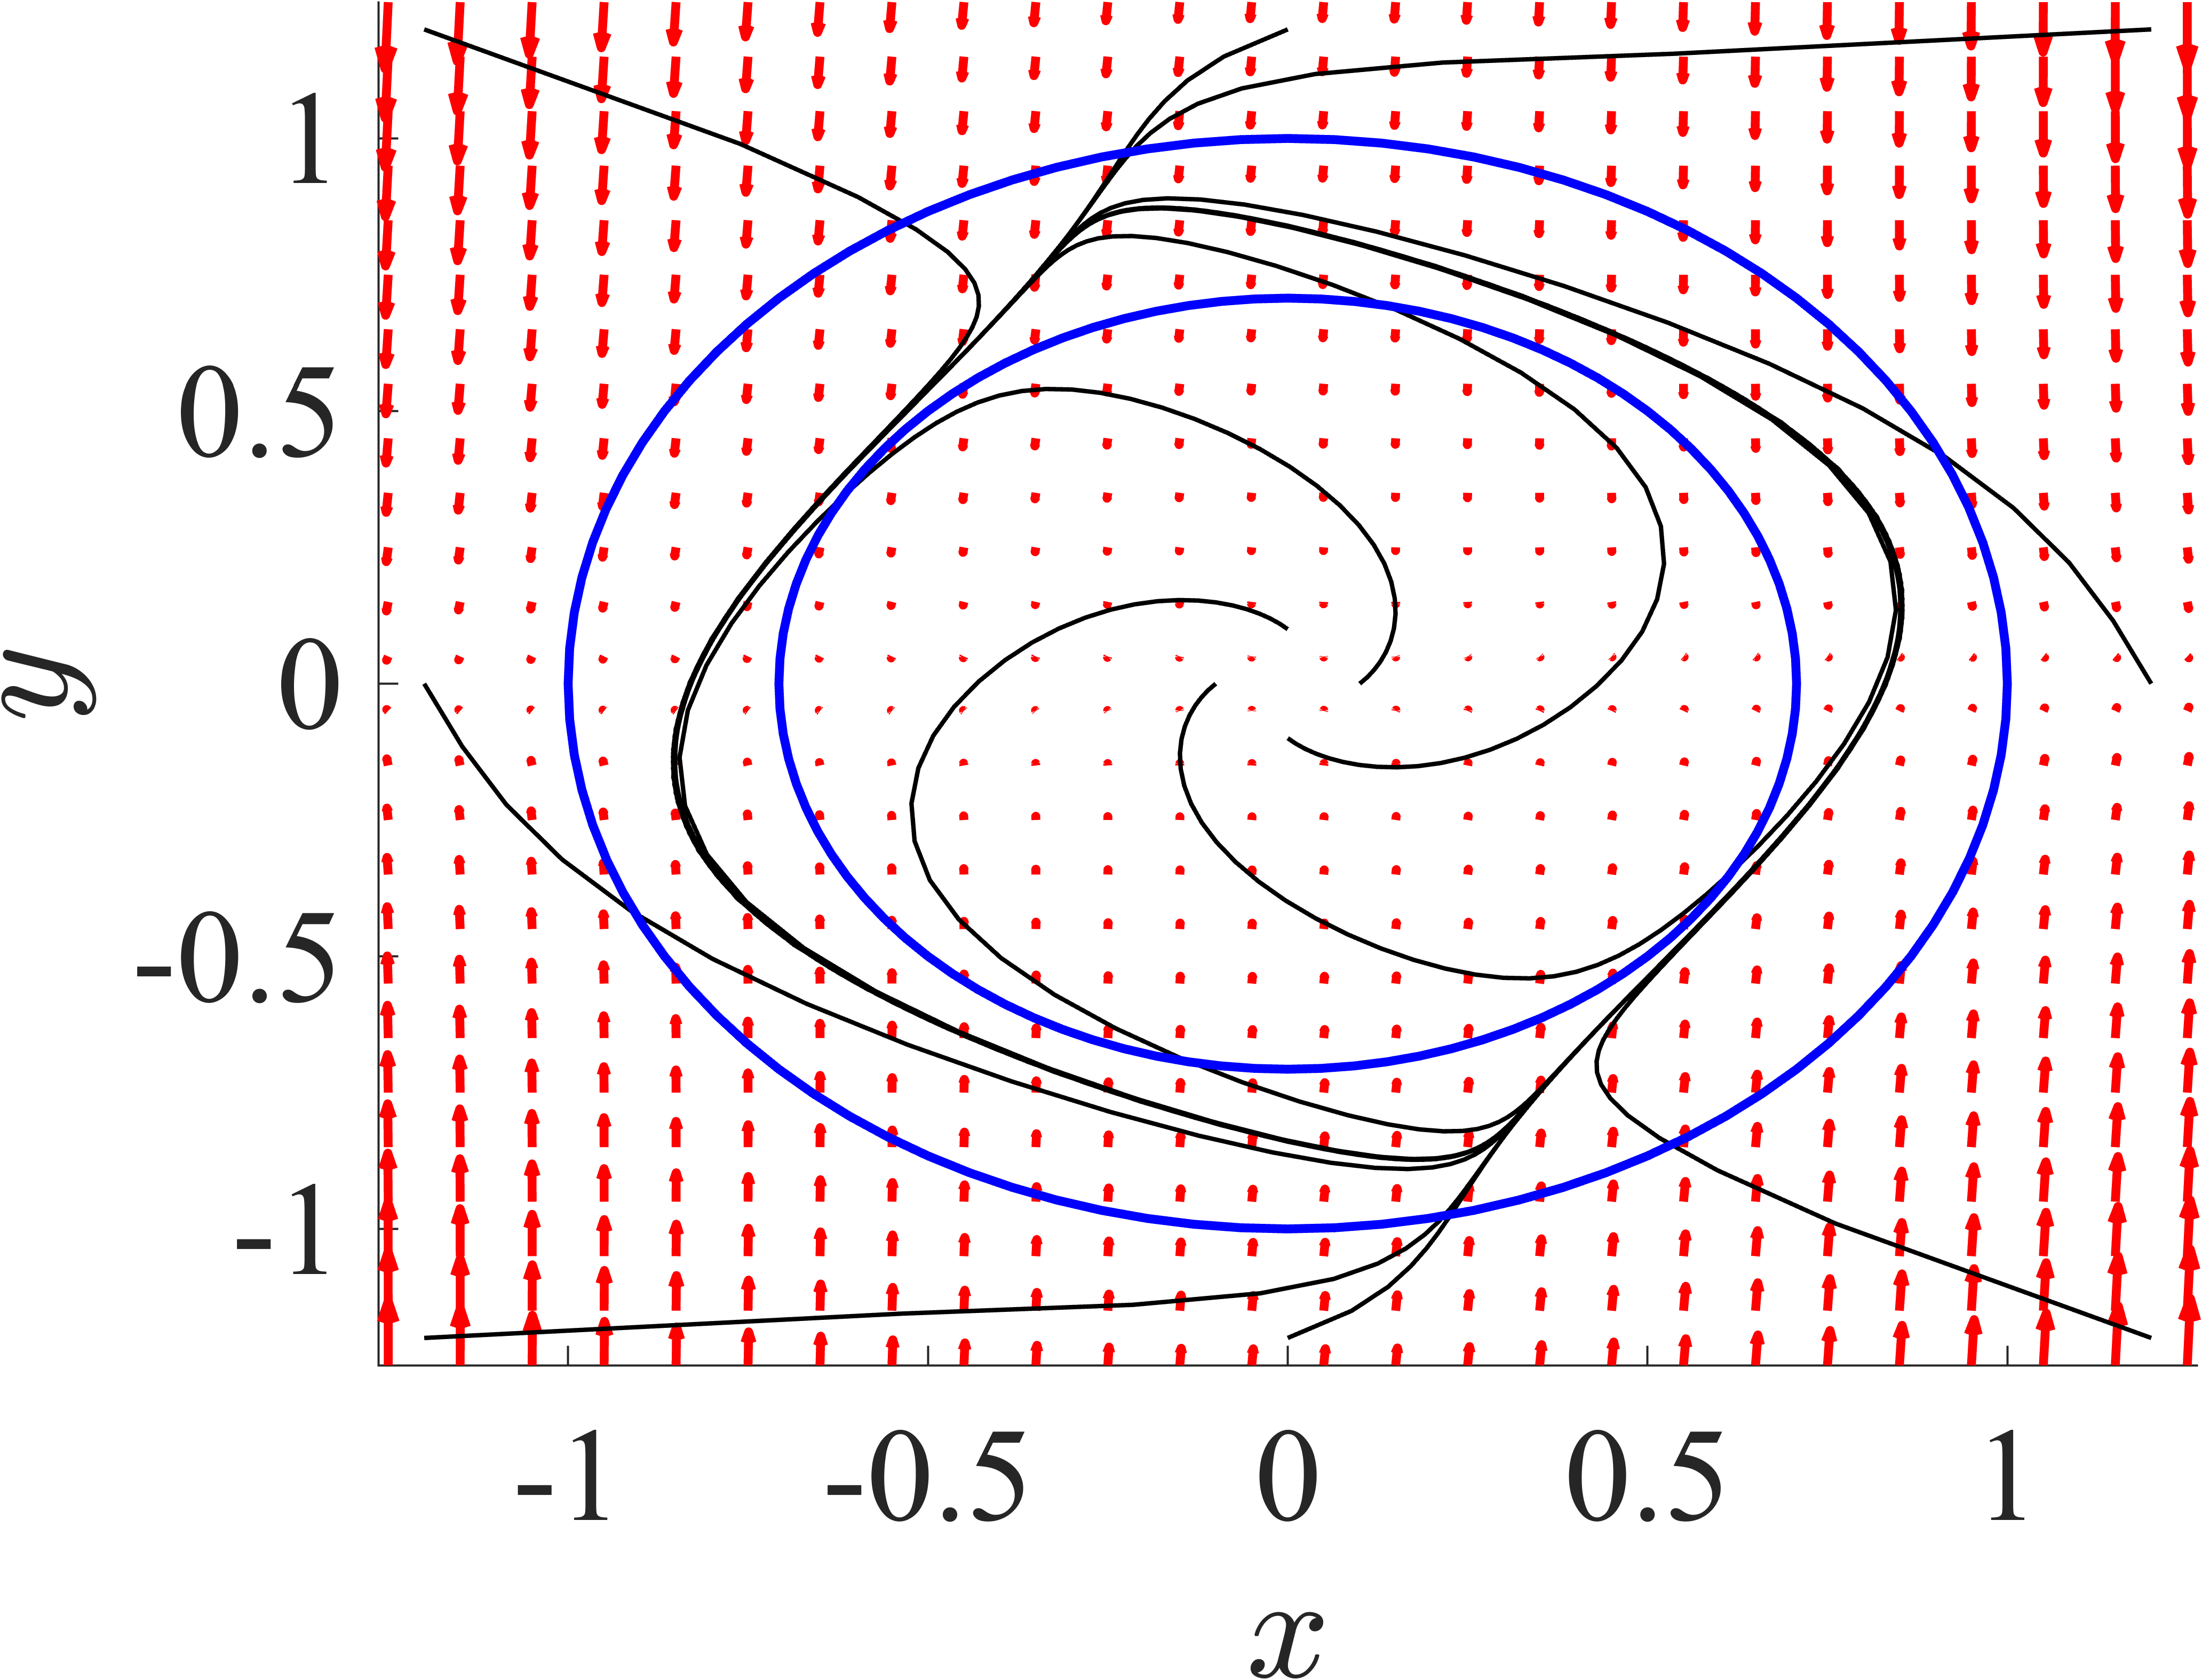
\includegraphics[width=8cm]{7.3.2_plot.png}
\caption{Phase Portrait}
\end{figure}

\section*{Problem 8.2.3}
The phase portraits for the system $\dot x = -y + \mu x + x y^2$ and $\dot y = x + \mu y - x^2$ are shown below. In these portraits, the blue dots are initial conditions. We see here that when $\mu < 0$, the center fixed point at the origin is stable. Furthermore, as $\mu$ increases from $-0.5$ to $-0.1$, the initial conditions far from the origin (such as the one at $(-0.9,0)$) start diverging from the origin. In addition, the spiral trajectories indicate that we may have a limit cycle. So what this implies is that there is a limit cycle that is unstable because trajectories starting inside the cycle converge to the origin and points starting outside the cycle diverge to infinity. Furthermore, when $\mu$ is further increased to $-0.05$ and to $-0.01$, we see that more and more of the trajectories start to diverge, and only trajectories that start very close to the origin still converge to a limit cycle. So the limit cycle is getting smaller and smaller as we approach $\mu = 0$. At the marginal case of $\mu = 0$, we just have an unstable spiral source at the origin. This behavior hints at a subcritical Hopf bifurcation because we have a stable fixed point and an unstable limit cycle that converge. 

We confirm this hypothesis when we see that at positive values of $\mu$, the origin becomes unstable and the unstable limit cycle disappears. This agrees with the behavior of a subcritical Hopf bifurcation. We also see that as $\mu$ increases, the solutions spiral less and less, and they begin to diverge more quickly. Note that a subcritical Hopf bifurcation also has a stable limit cycle that is stable regardless of $\mu$, but we are not seeing it in the plots. This may be because the stable limit cycle is far from the origin.

\begin{figure}[h]
\centering
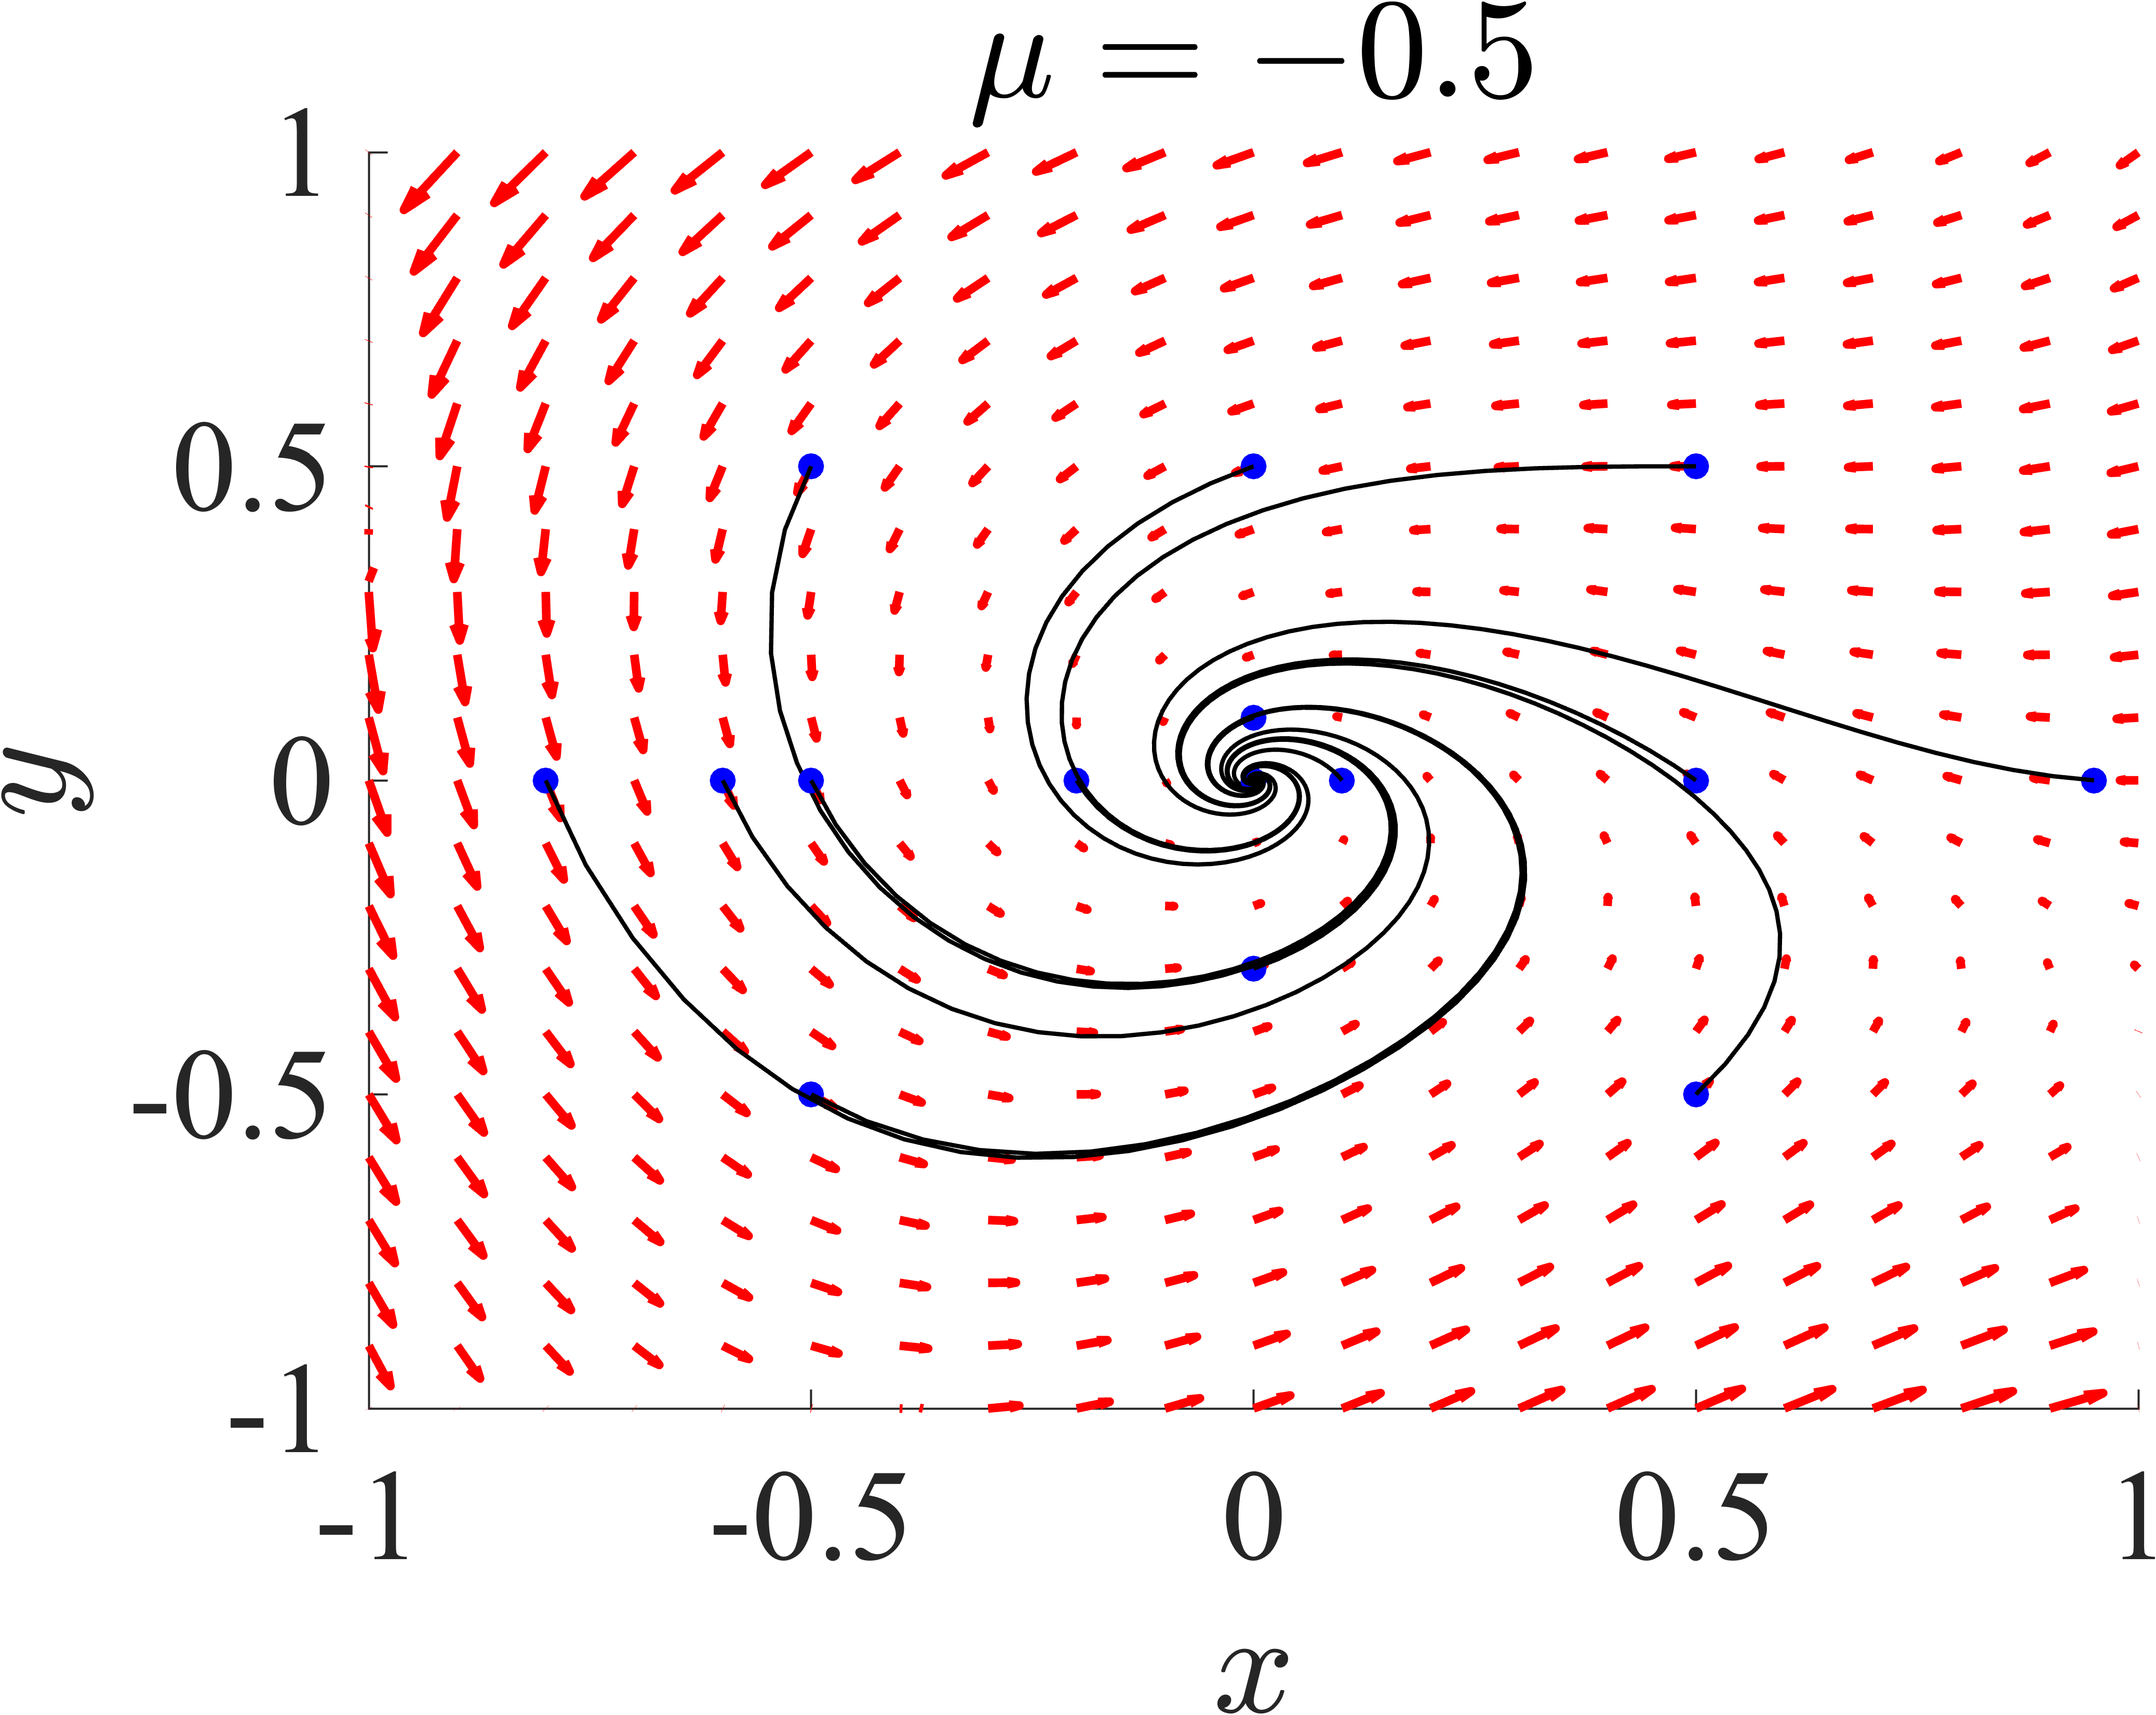
\includegraphics[width=7cm]{Hopf_823_phase_mu-0.5.png}
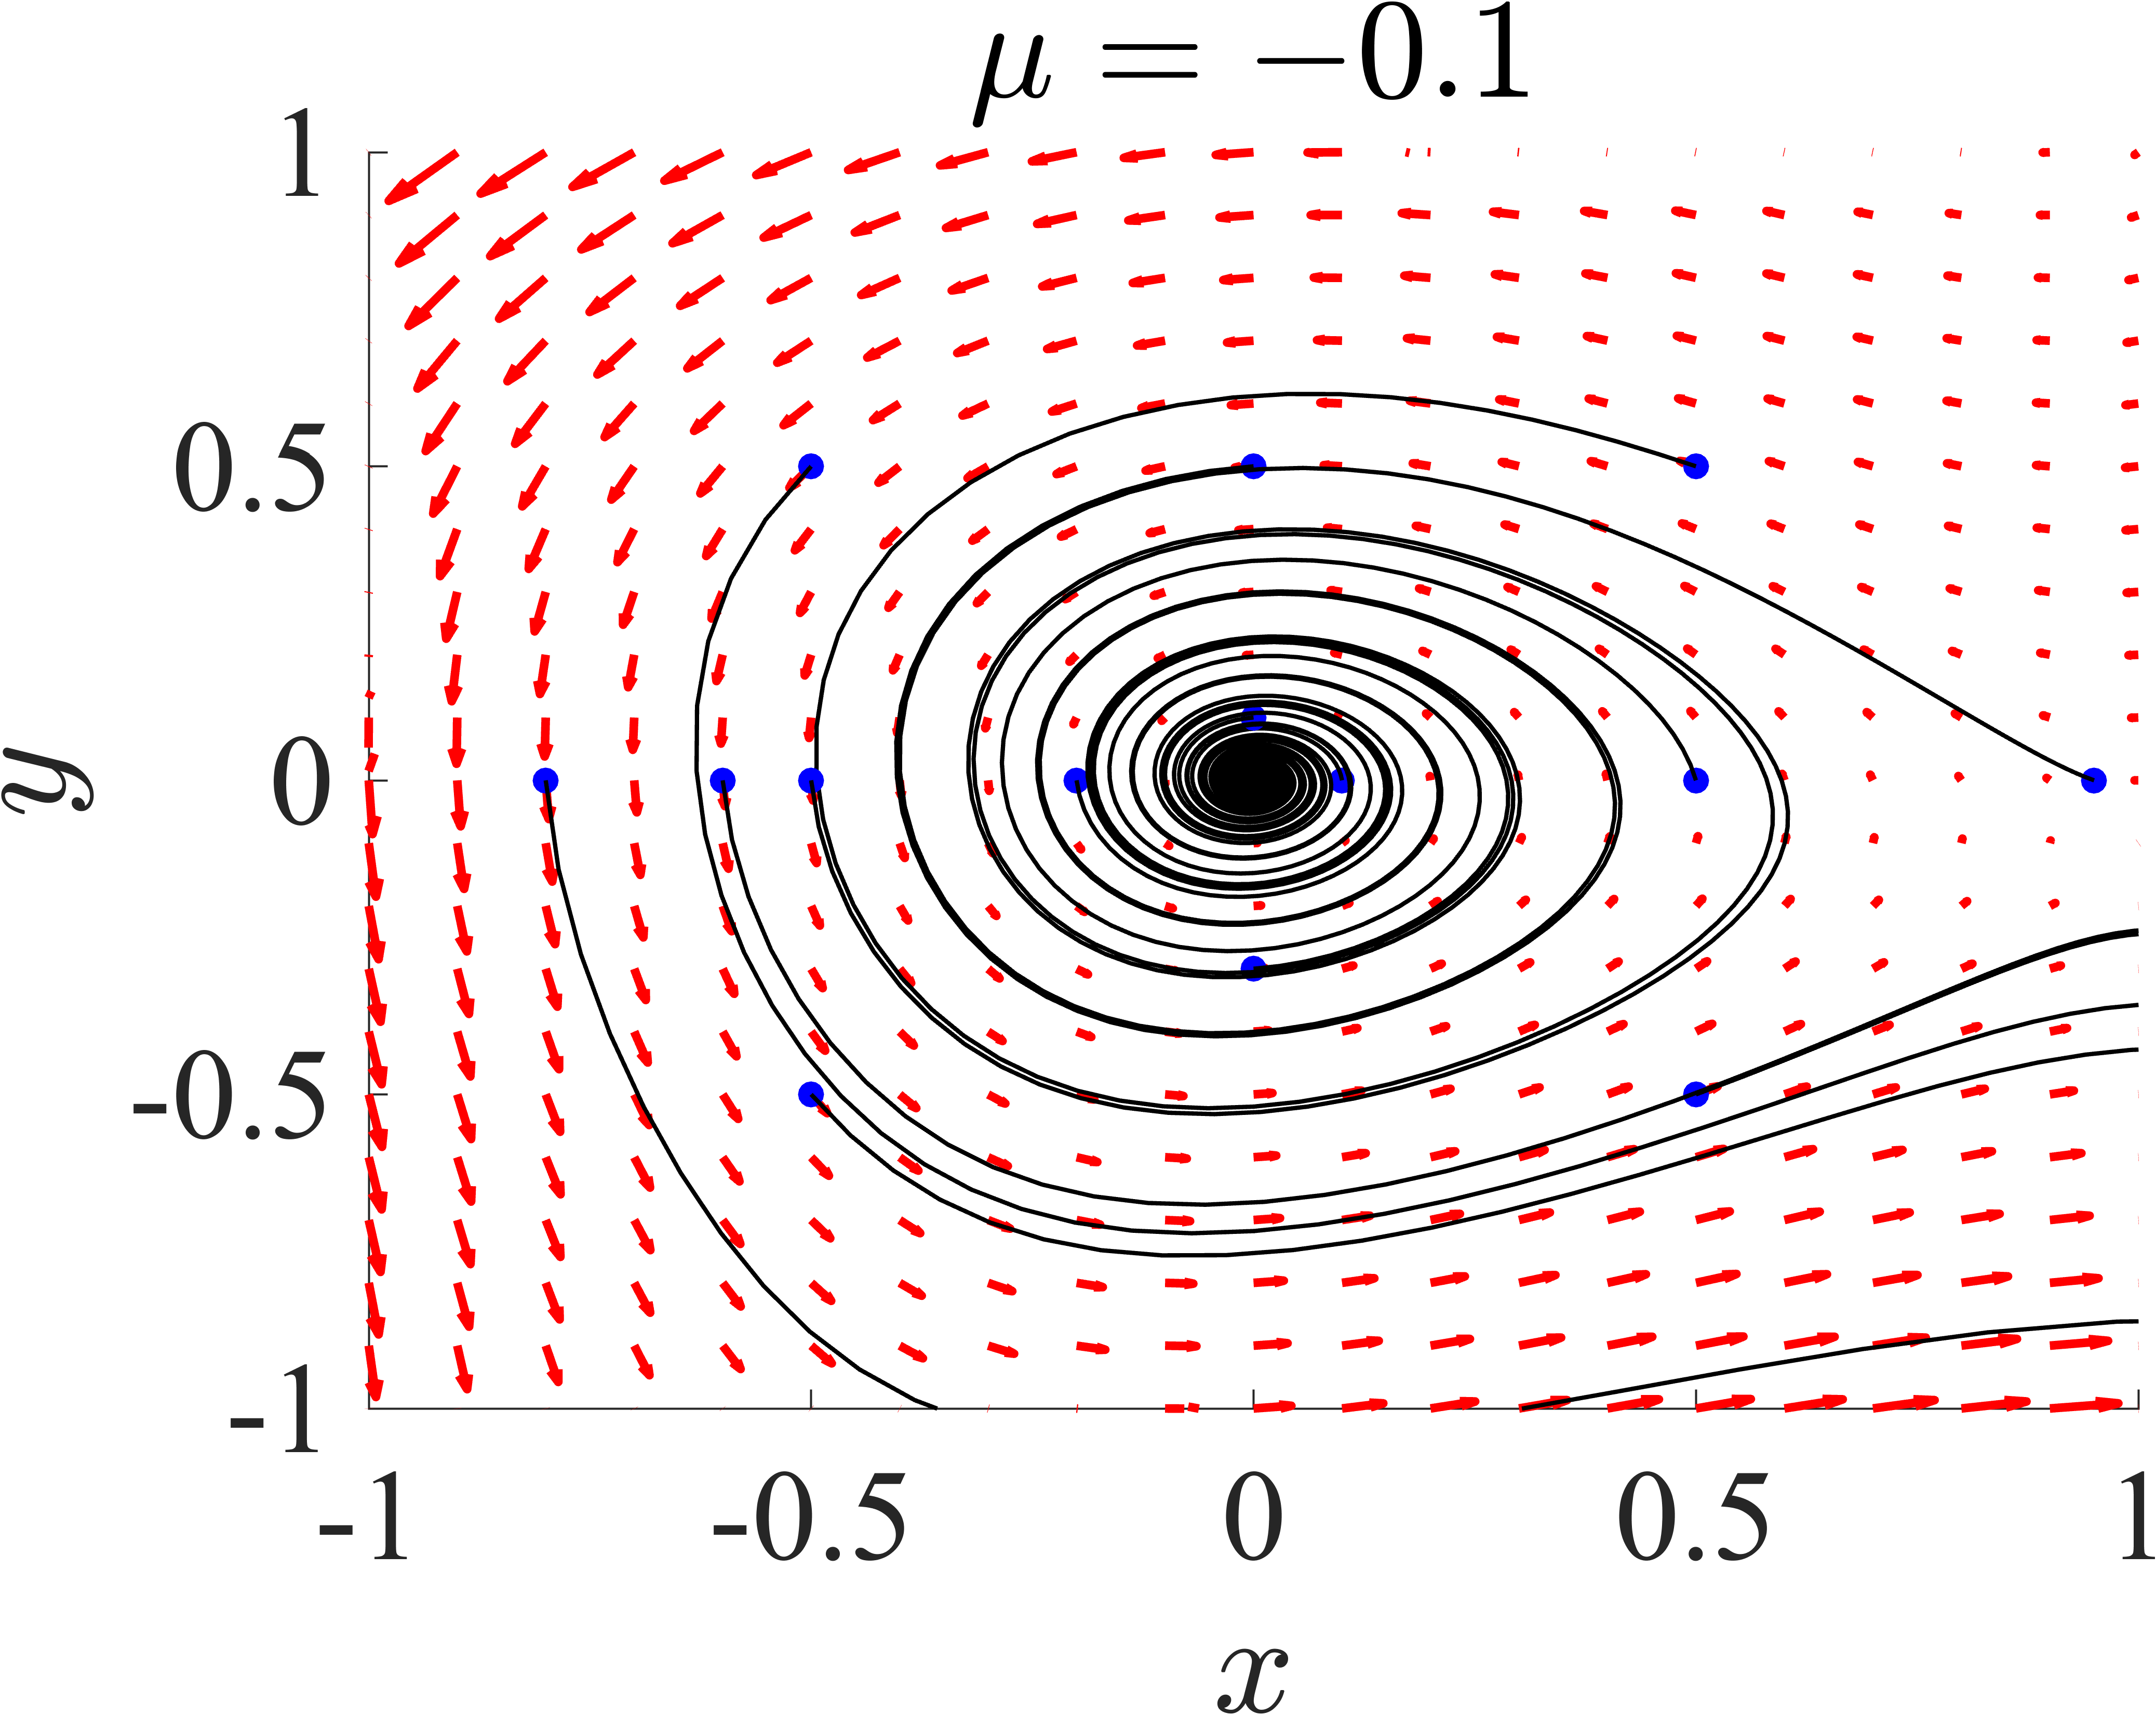
\includegraphics[width=7cm]{Hopf_823_phase_mu-0.1.png}
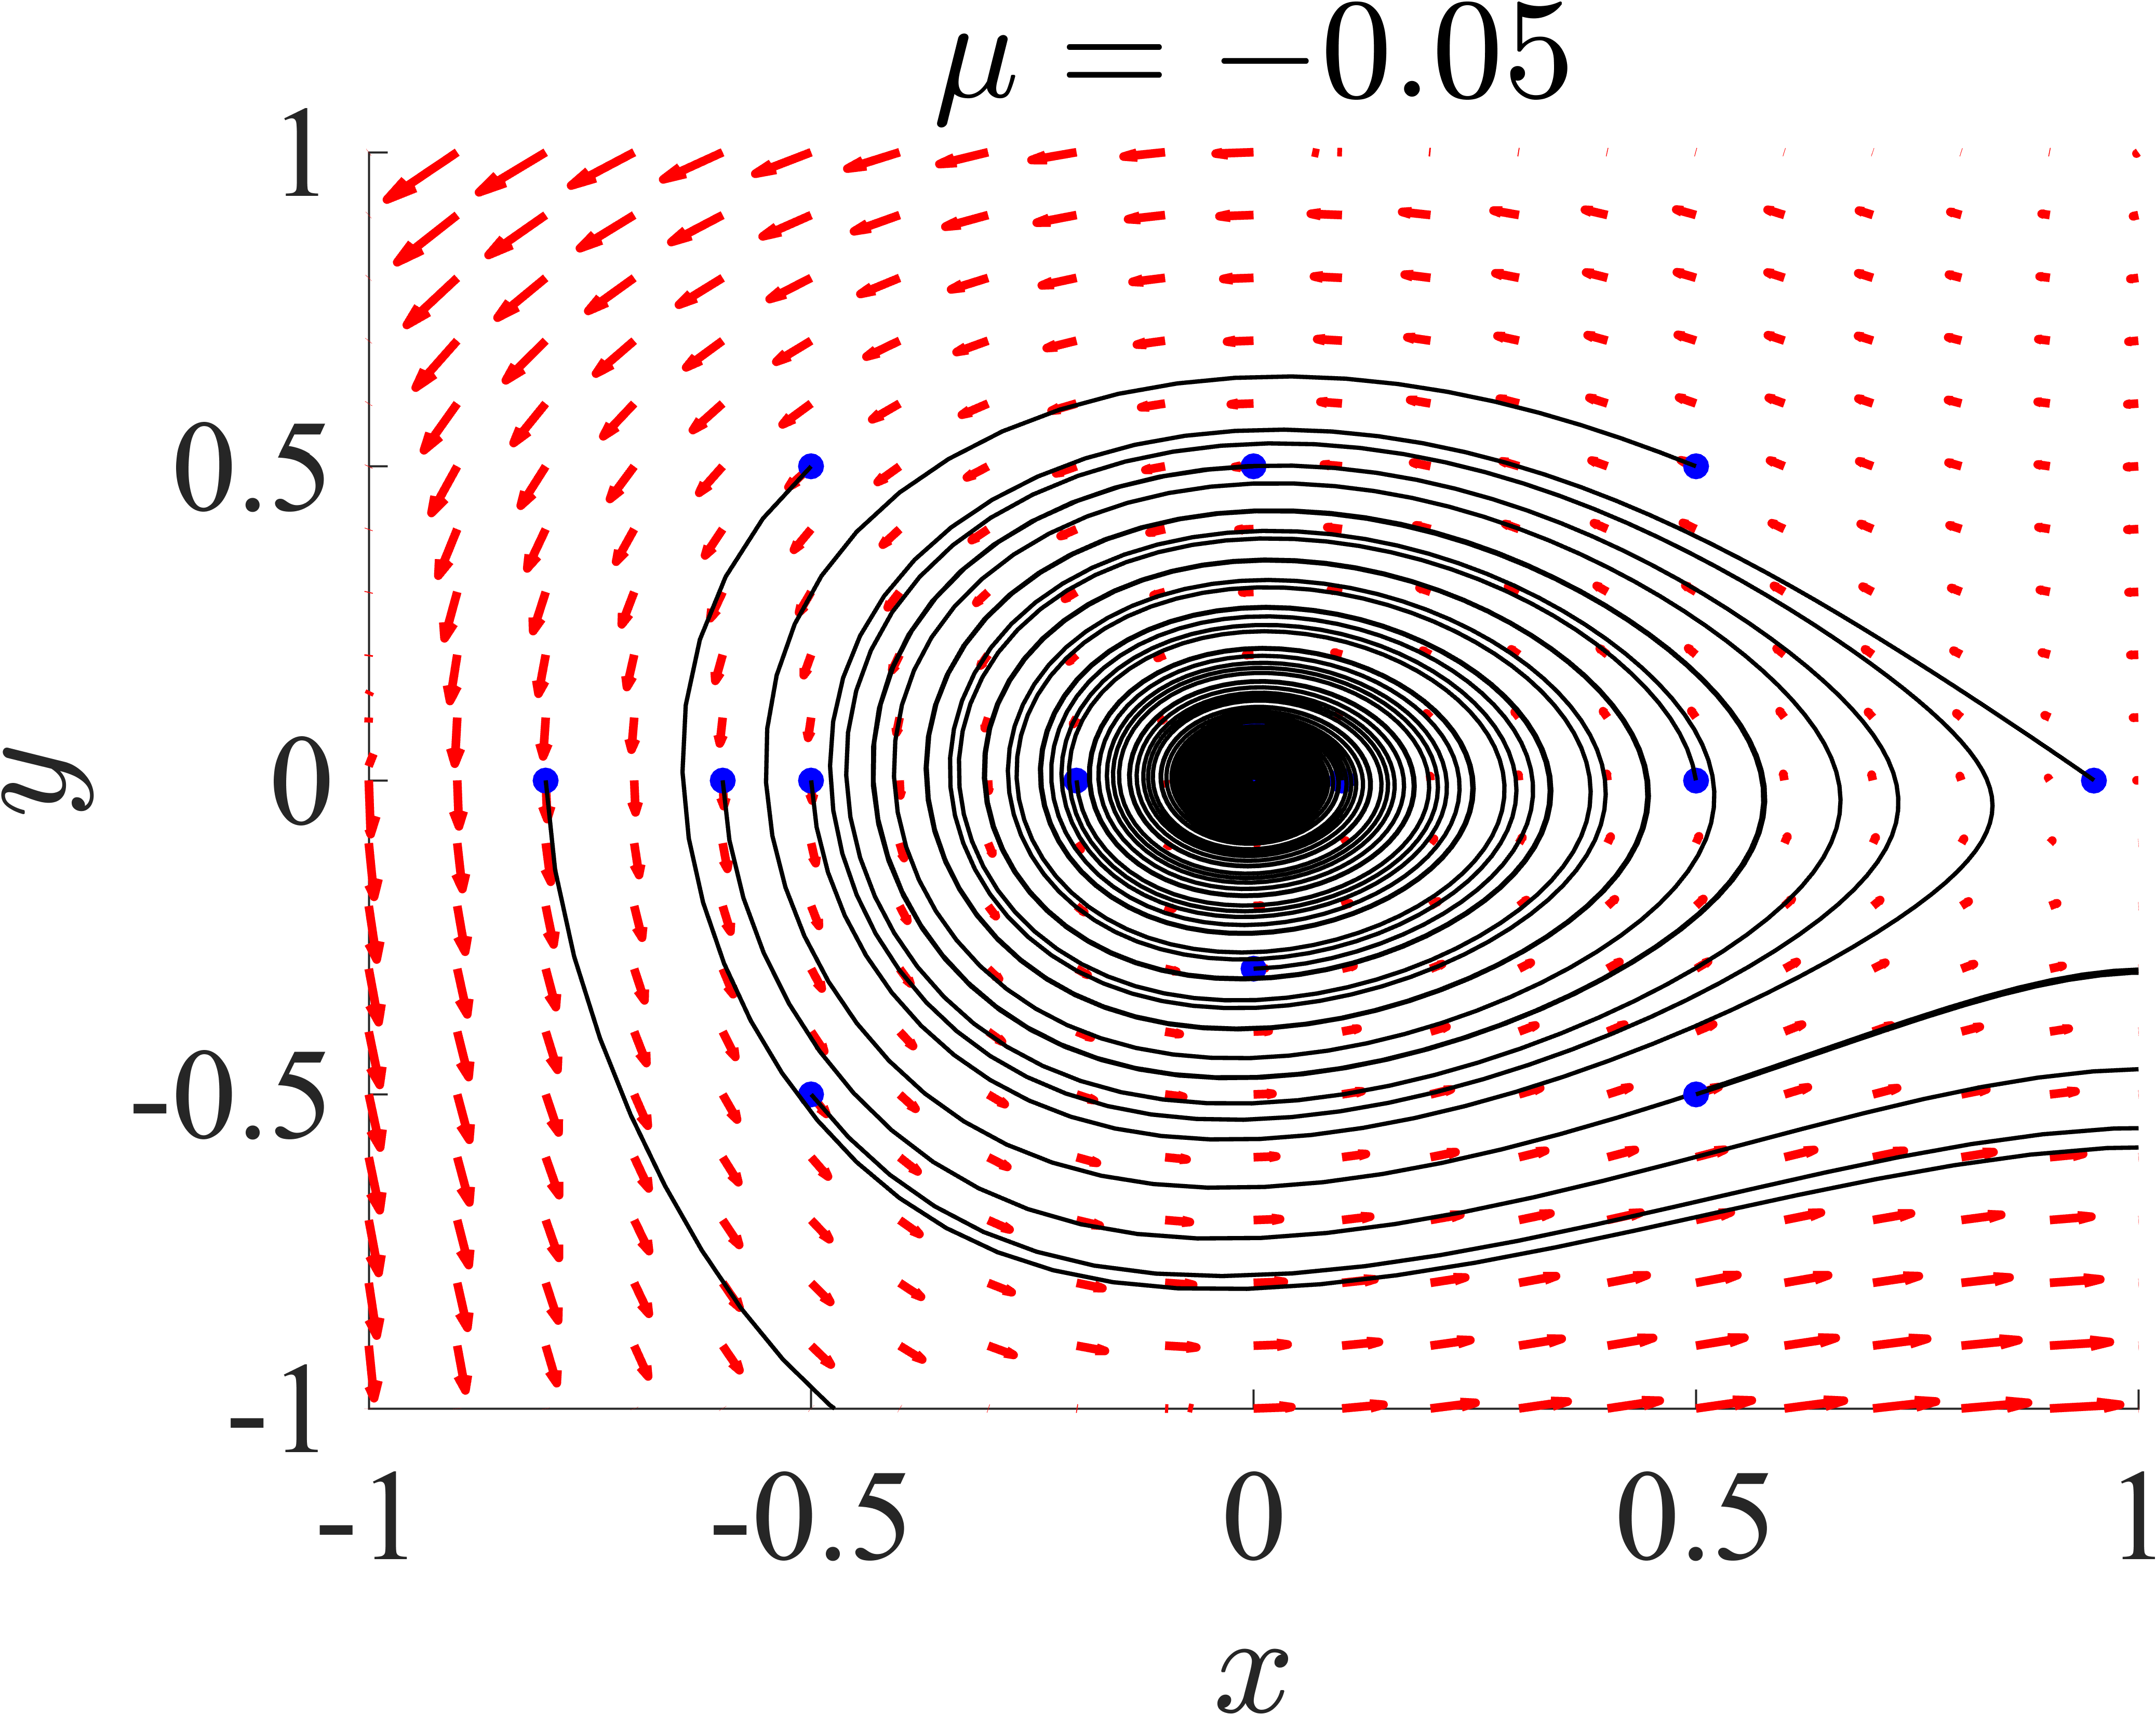
\includegraphics[width=7cm]{Hopf_823_phase_mu-0.05.png}
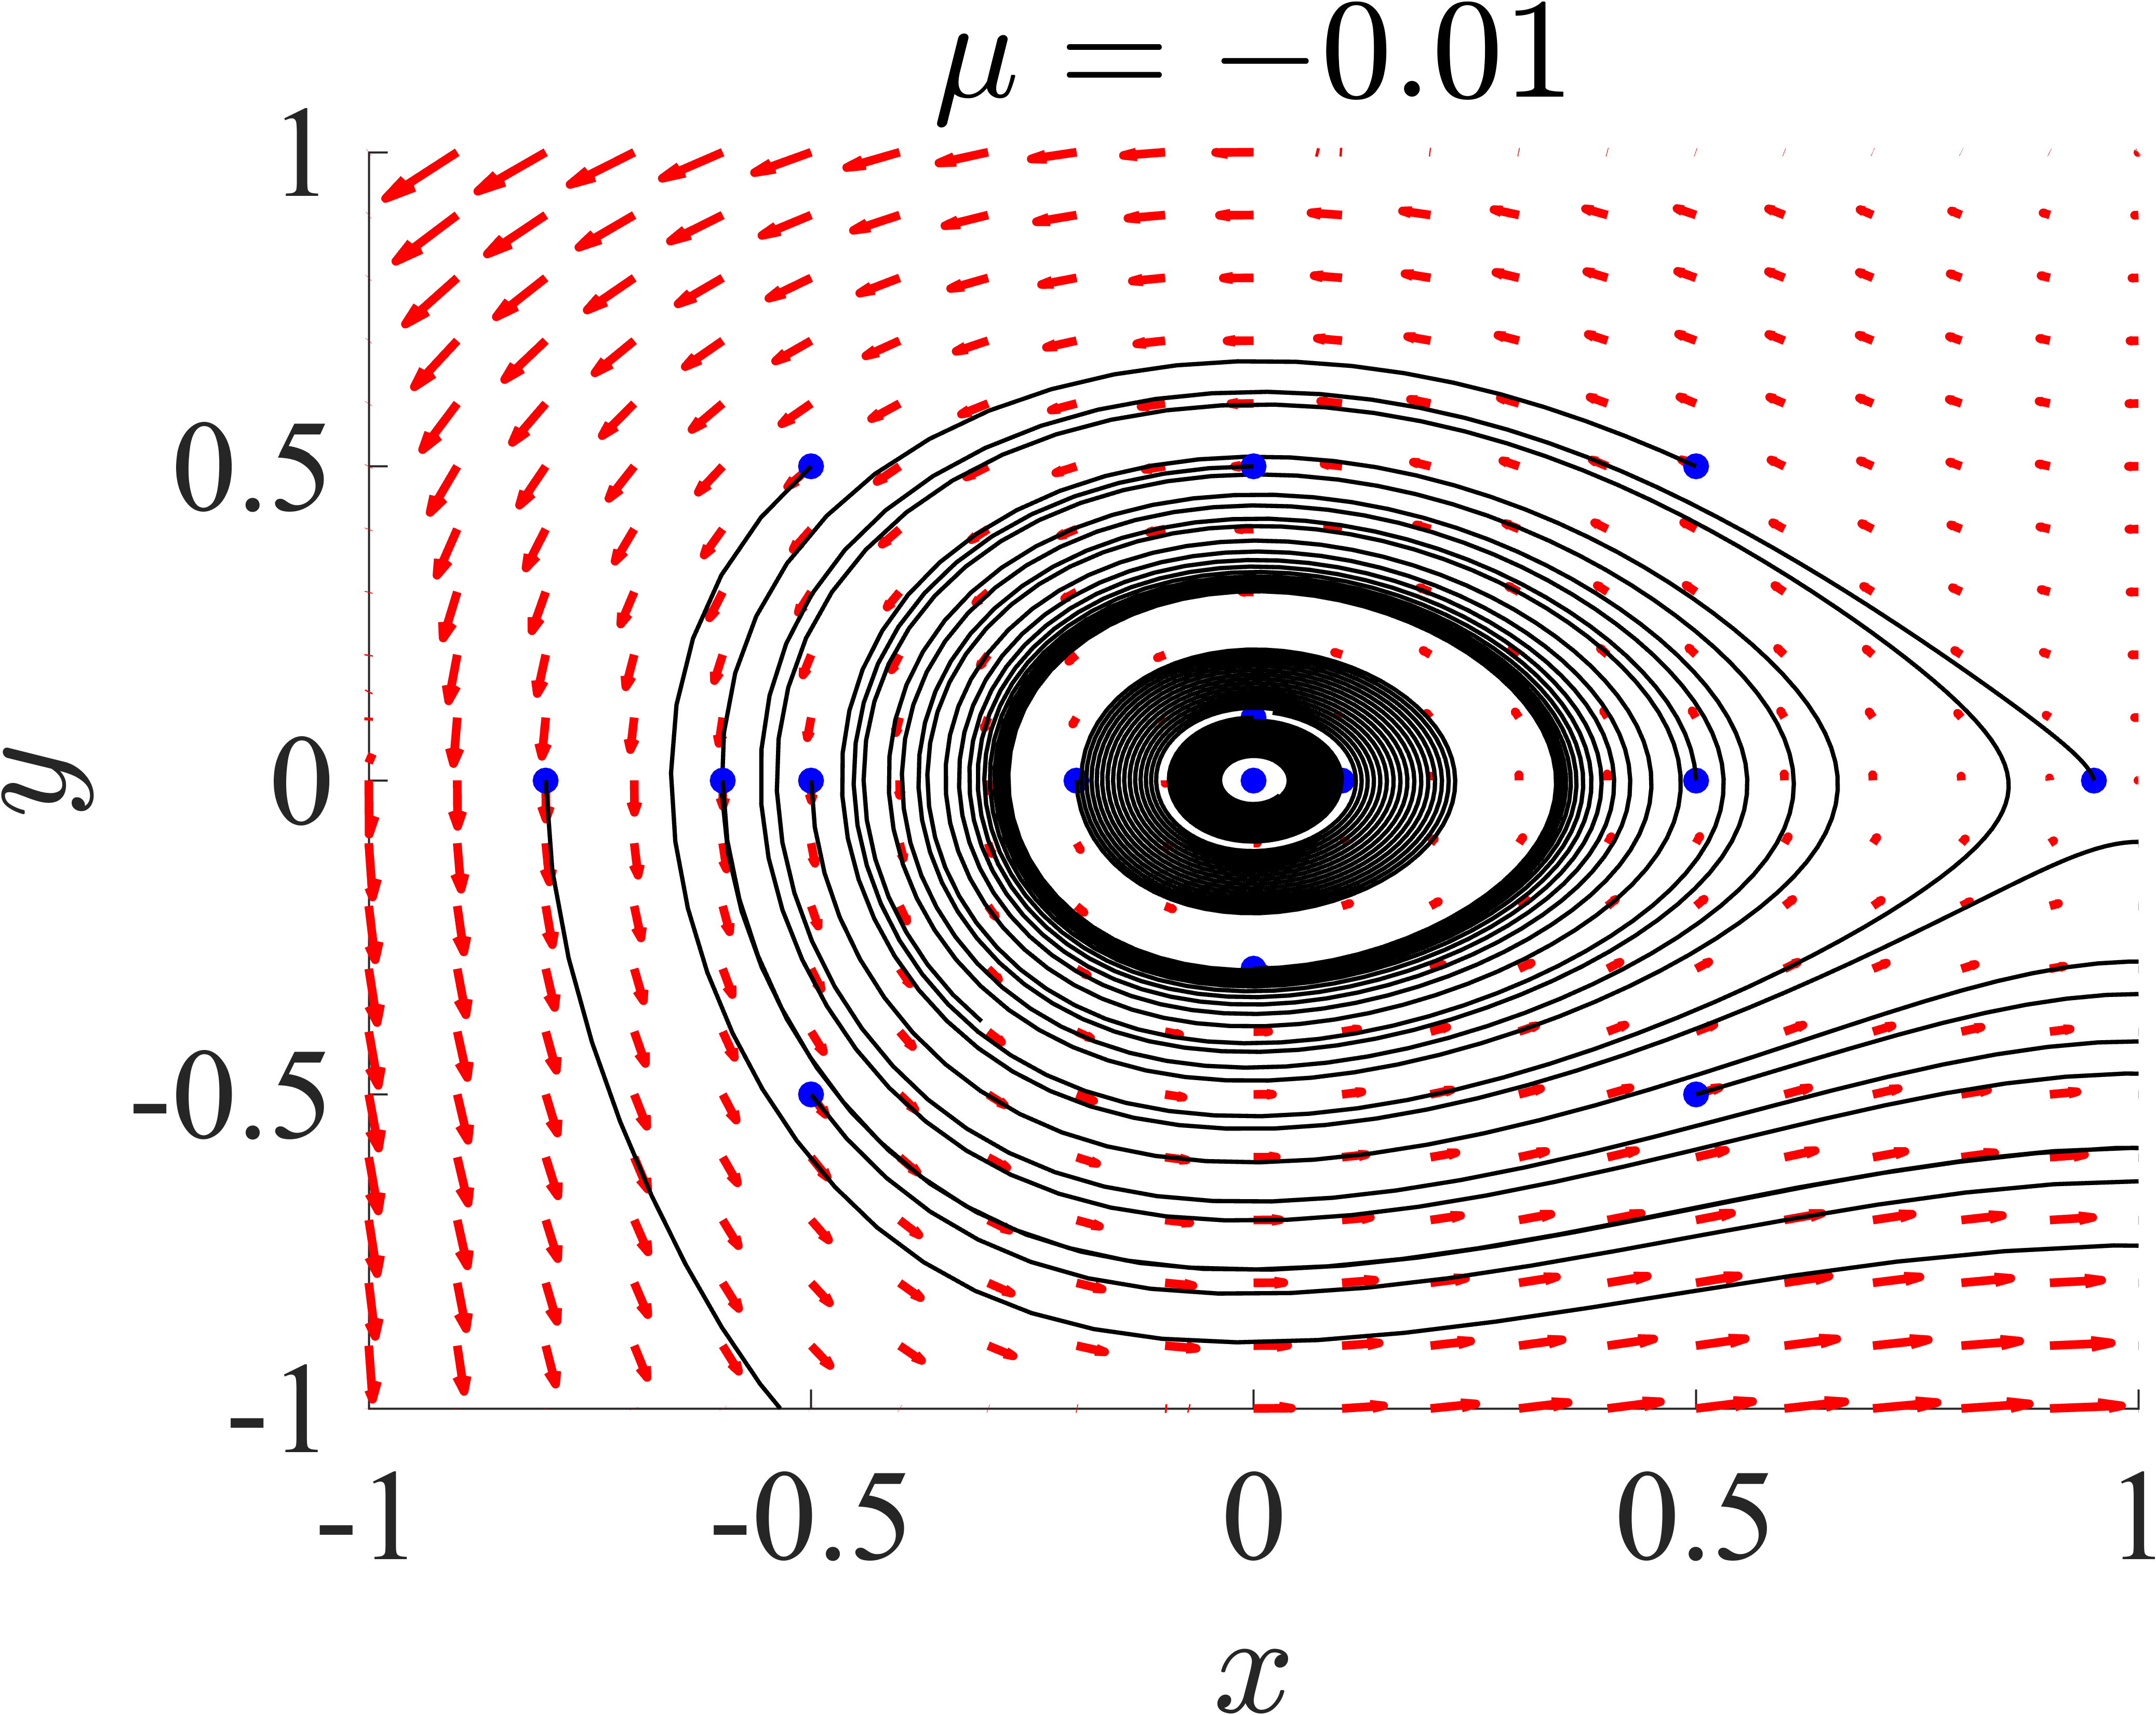
\includegraphics[width=7cm]{Hopf_823_phase_mu-0.01.png}
\caption{Phase Portraits for $\mu < 0$}
\end{figure}

\begin{figure}[h]
\centering
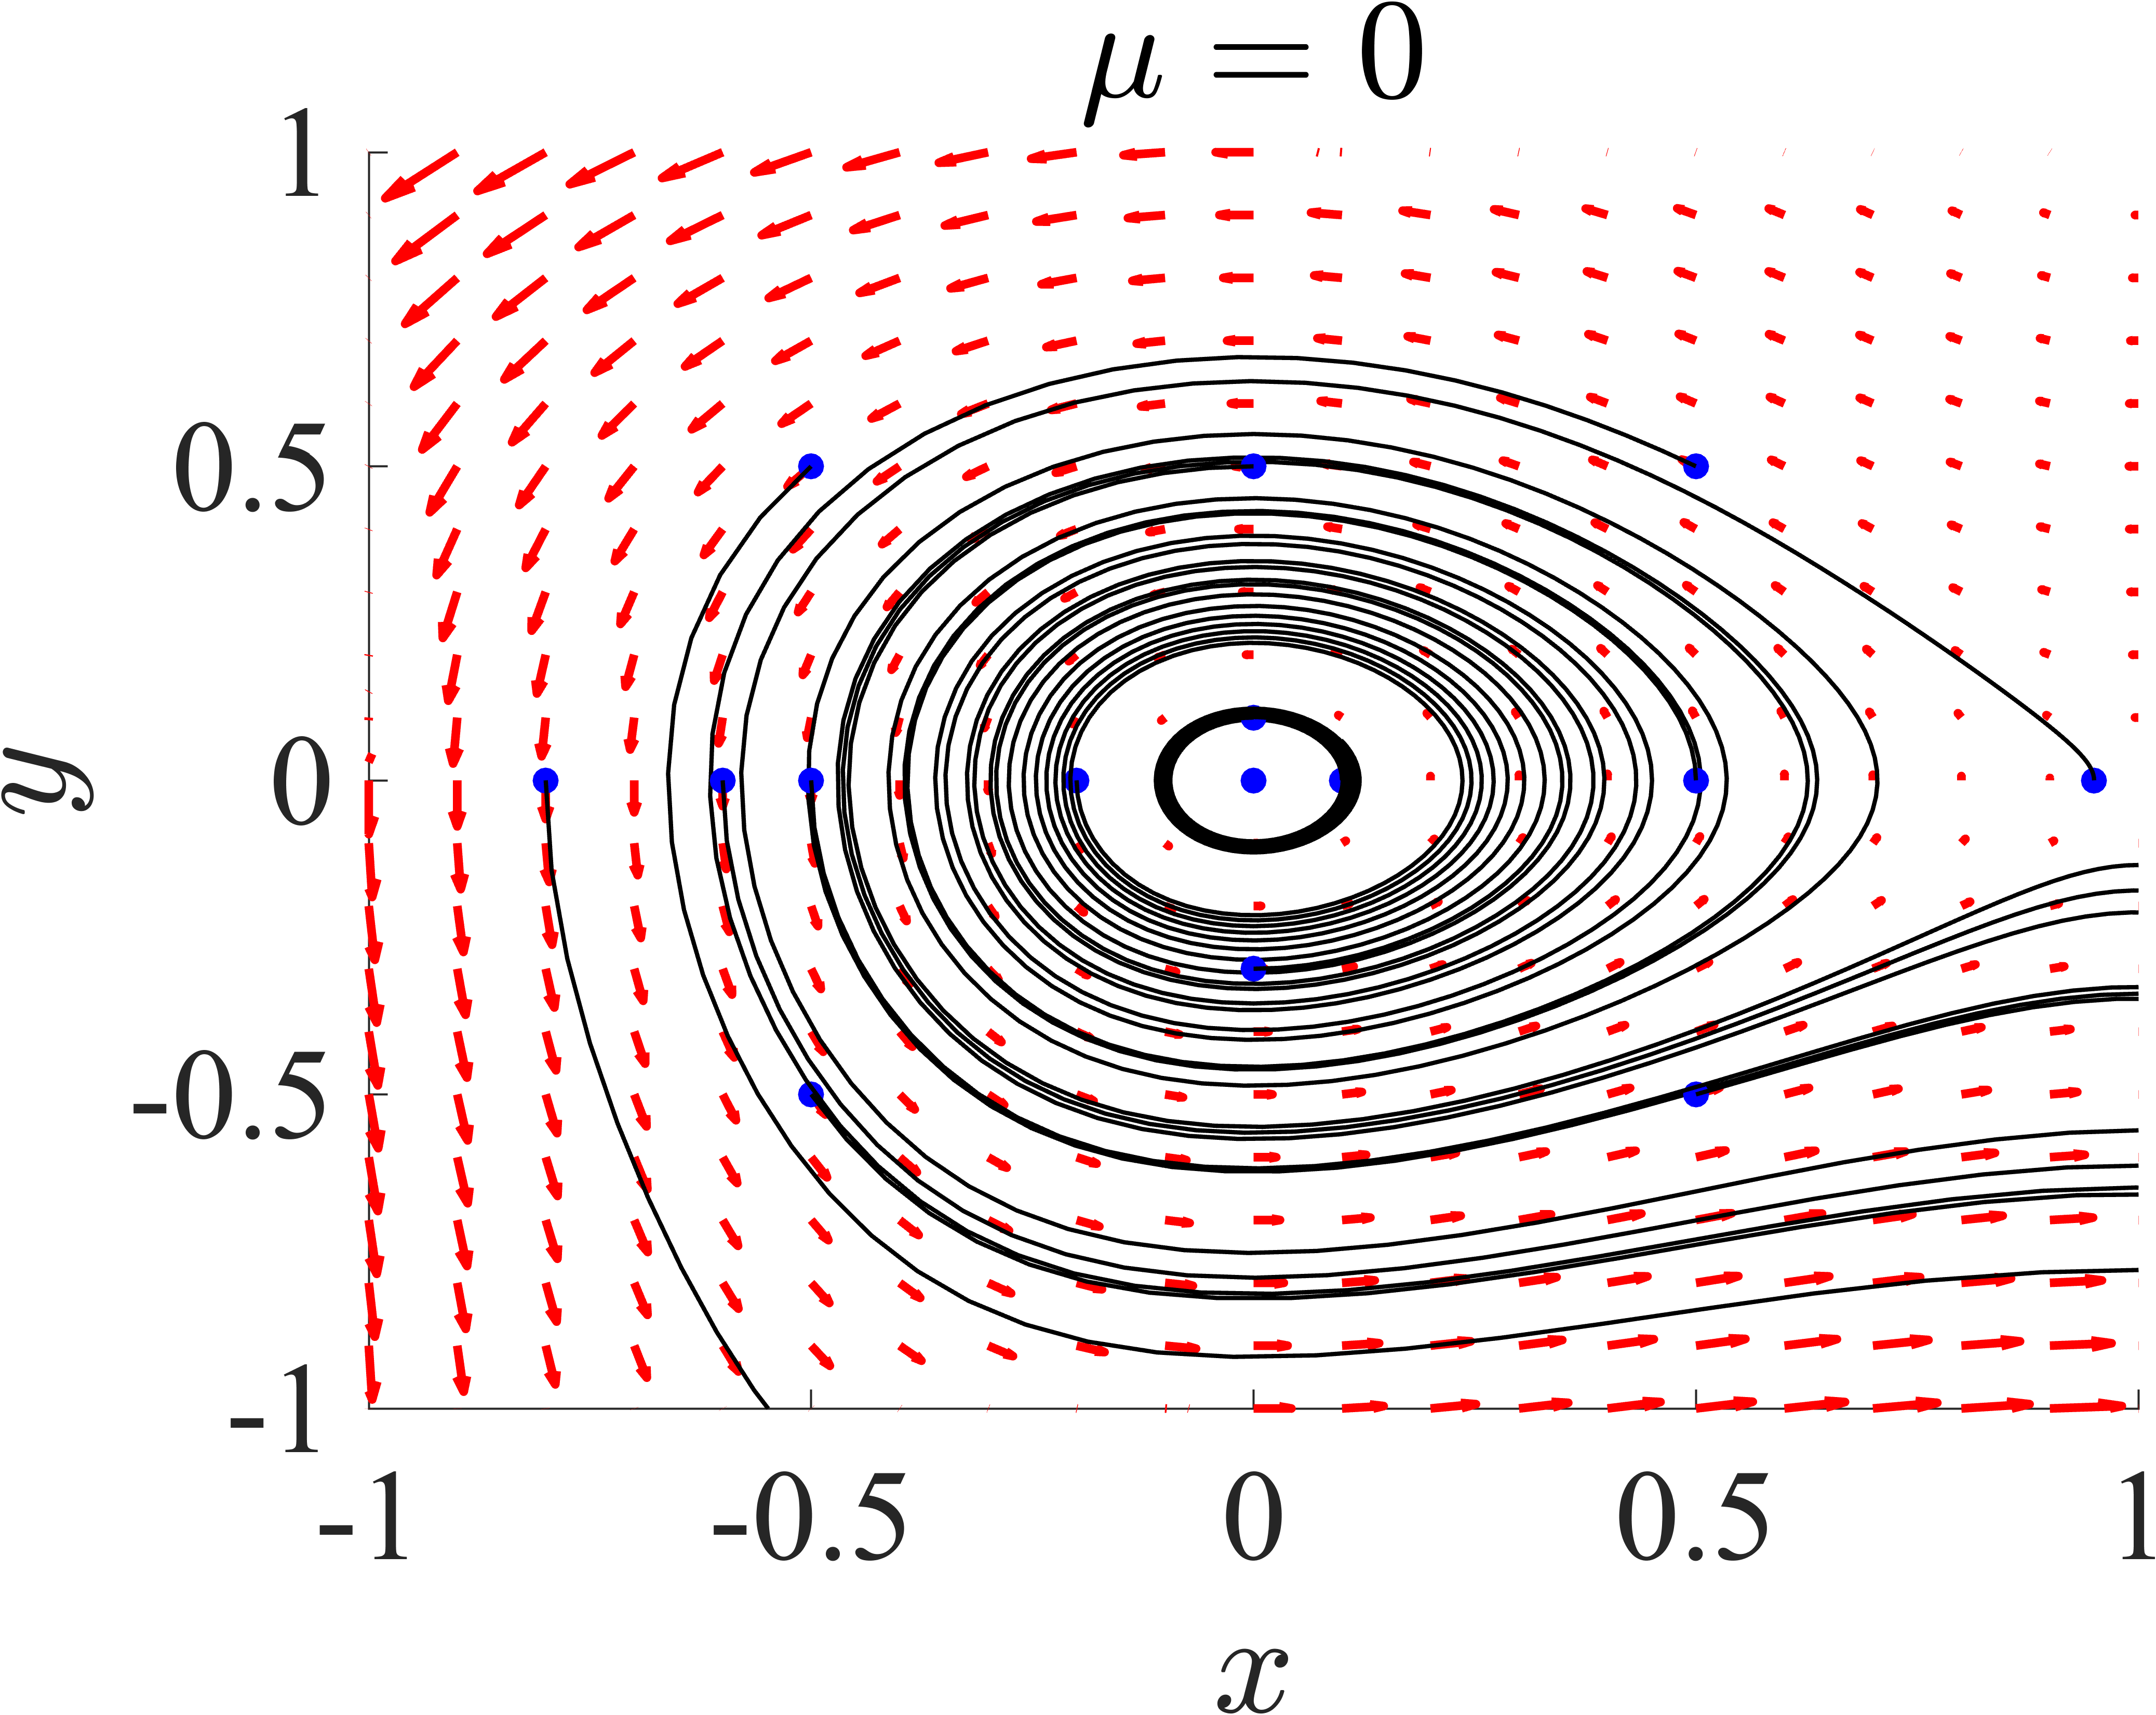
\includegraphics[width=7cm]{Hopf_823_phase_mu0.png}
\caption{Phase Portrait for $\mu = 0$}
\end{figure}

\begin{figure}[h]
\centering
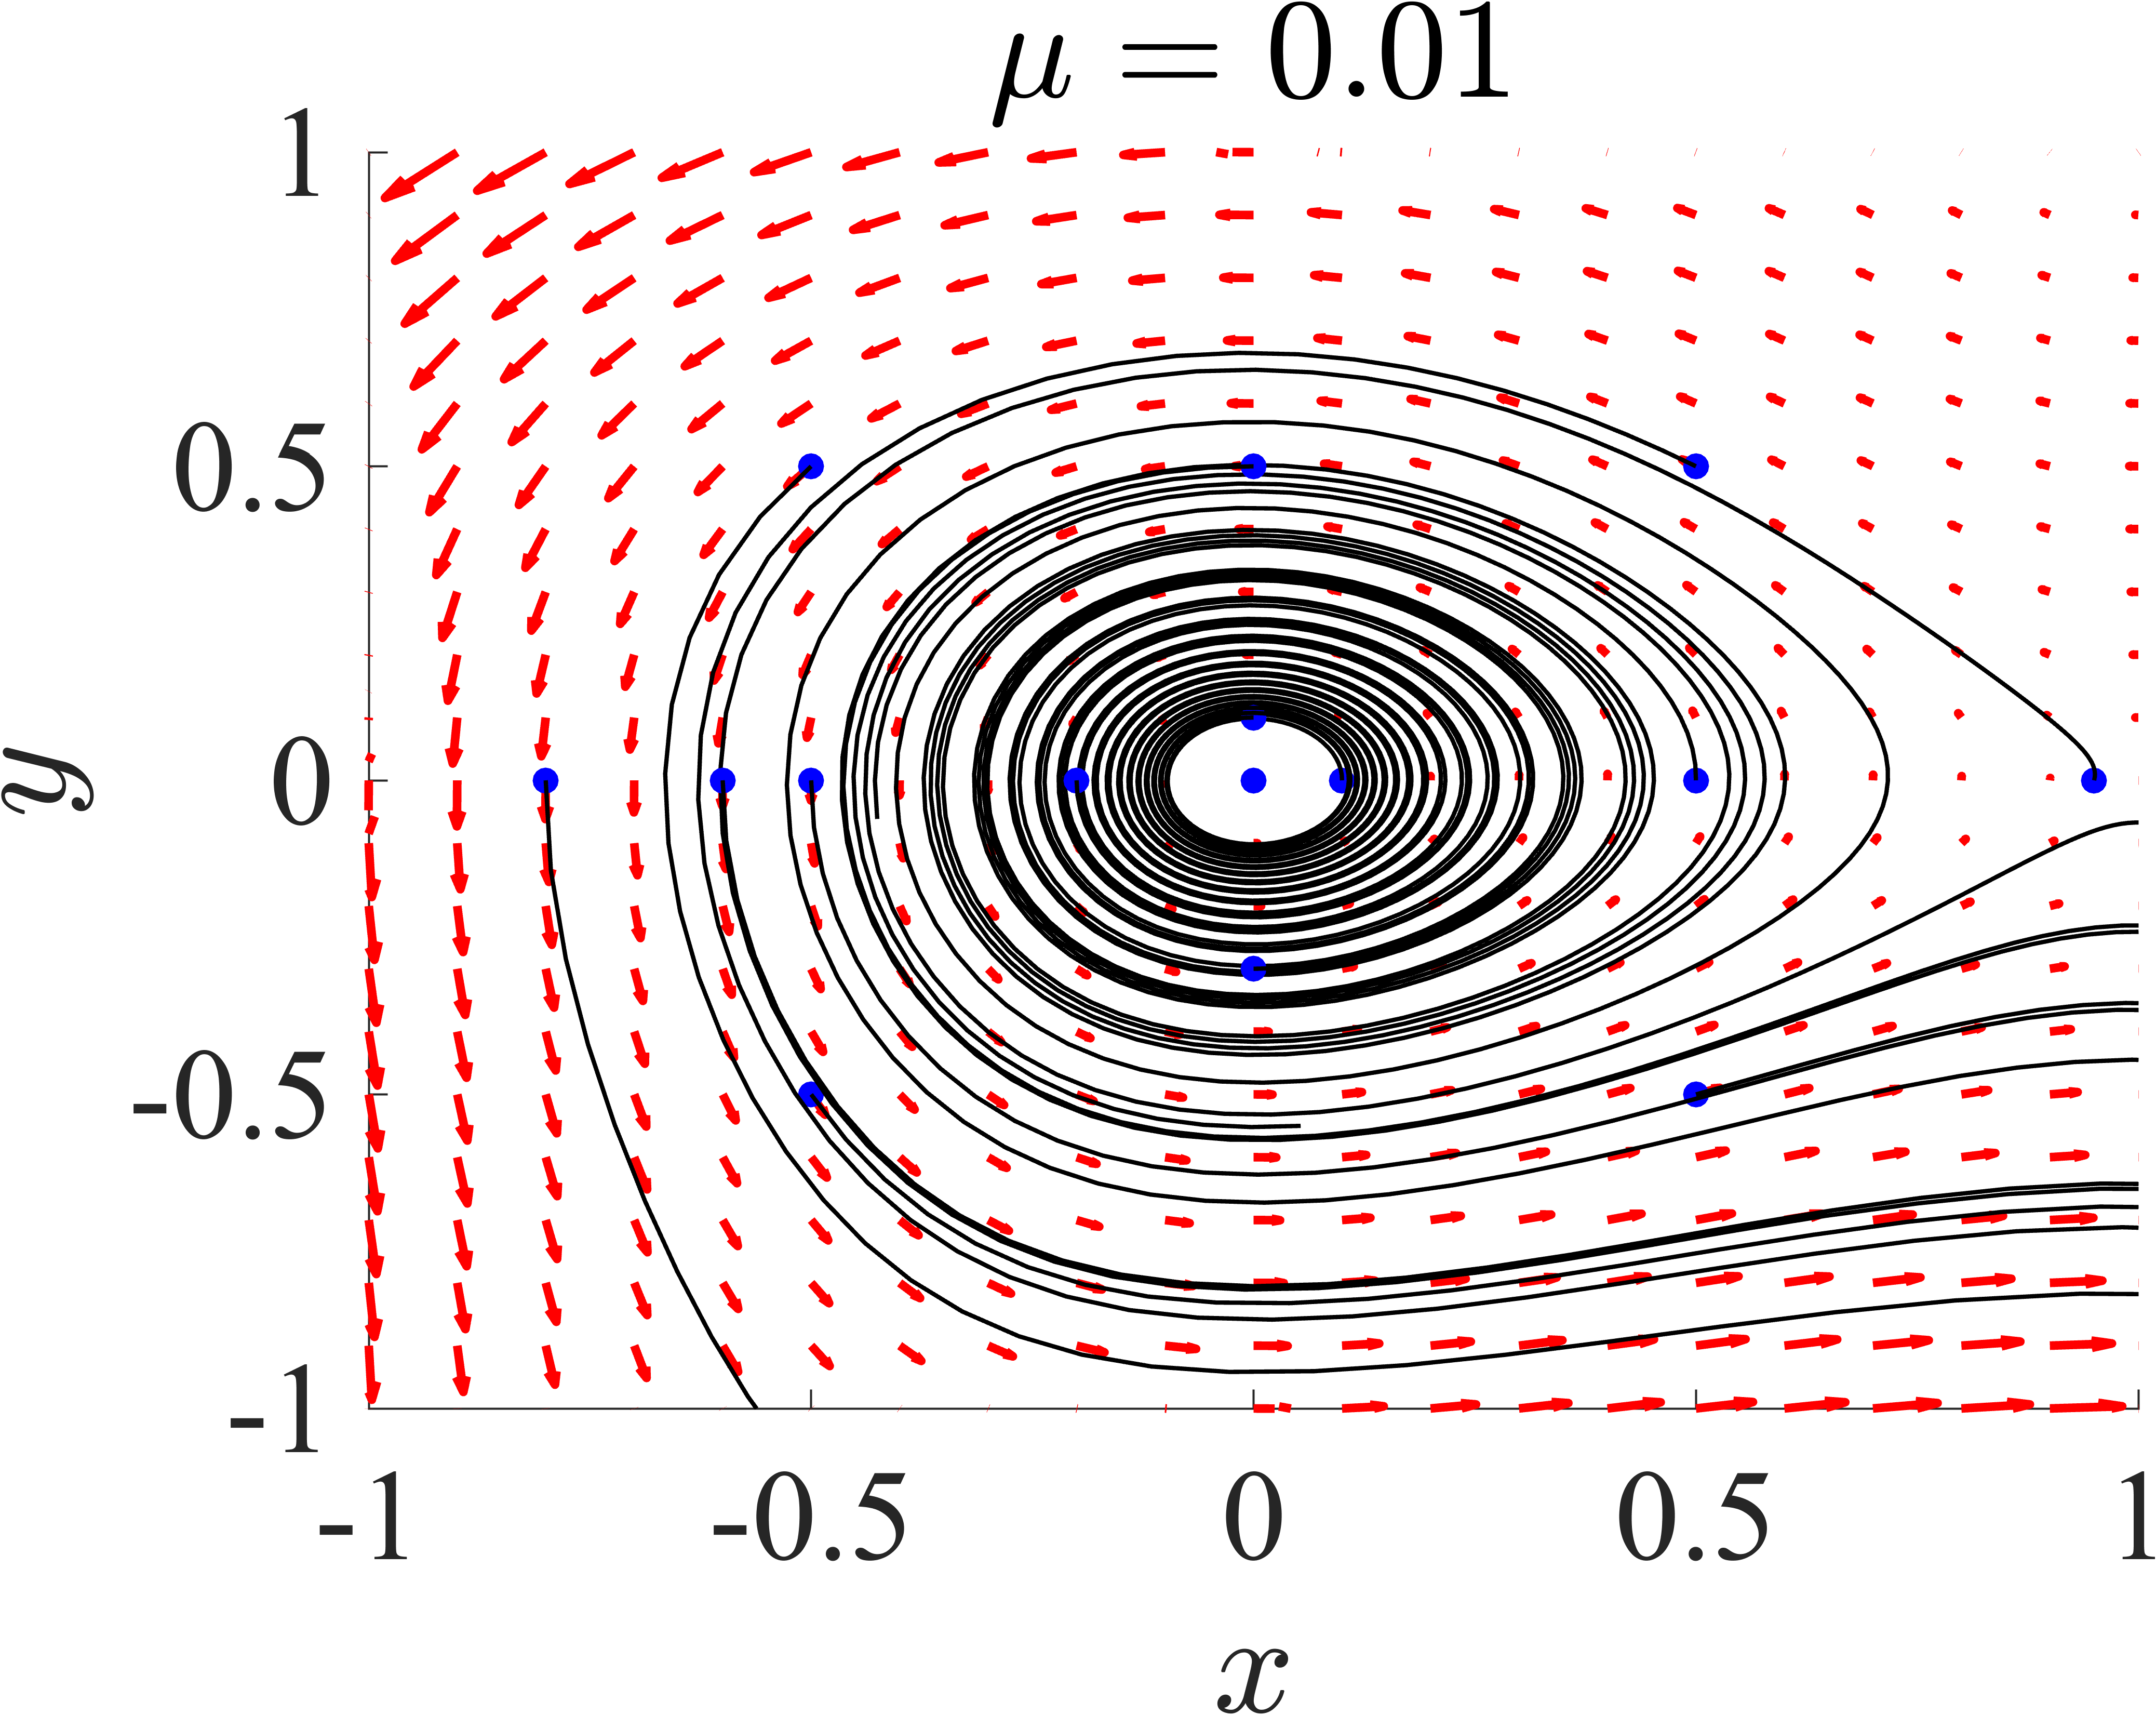
\includegraphics[width=7cm]{Hopf_823_phase_mu0.01.png}
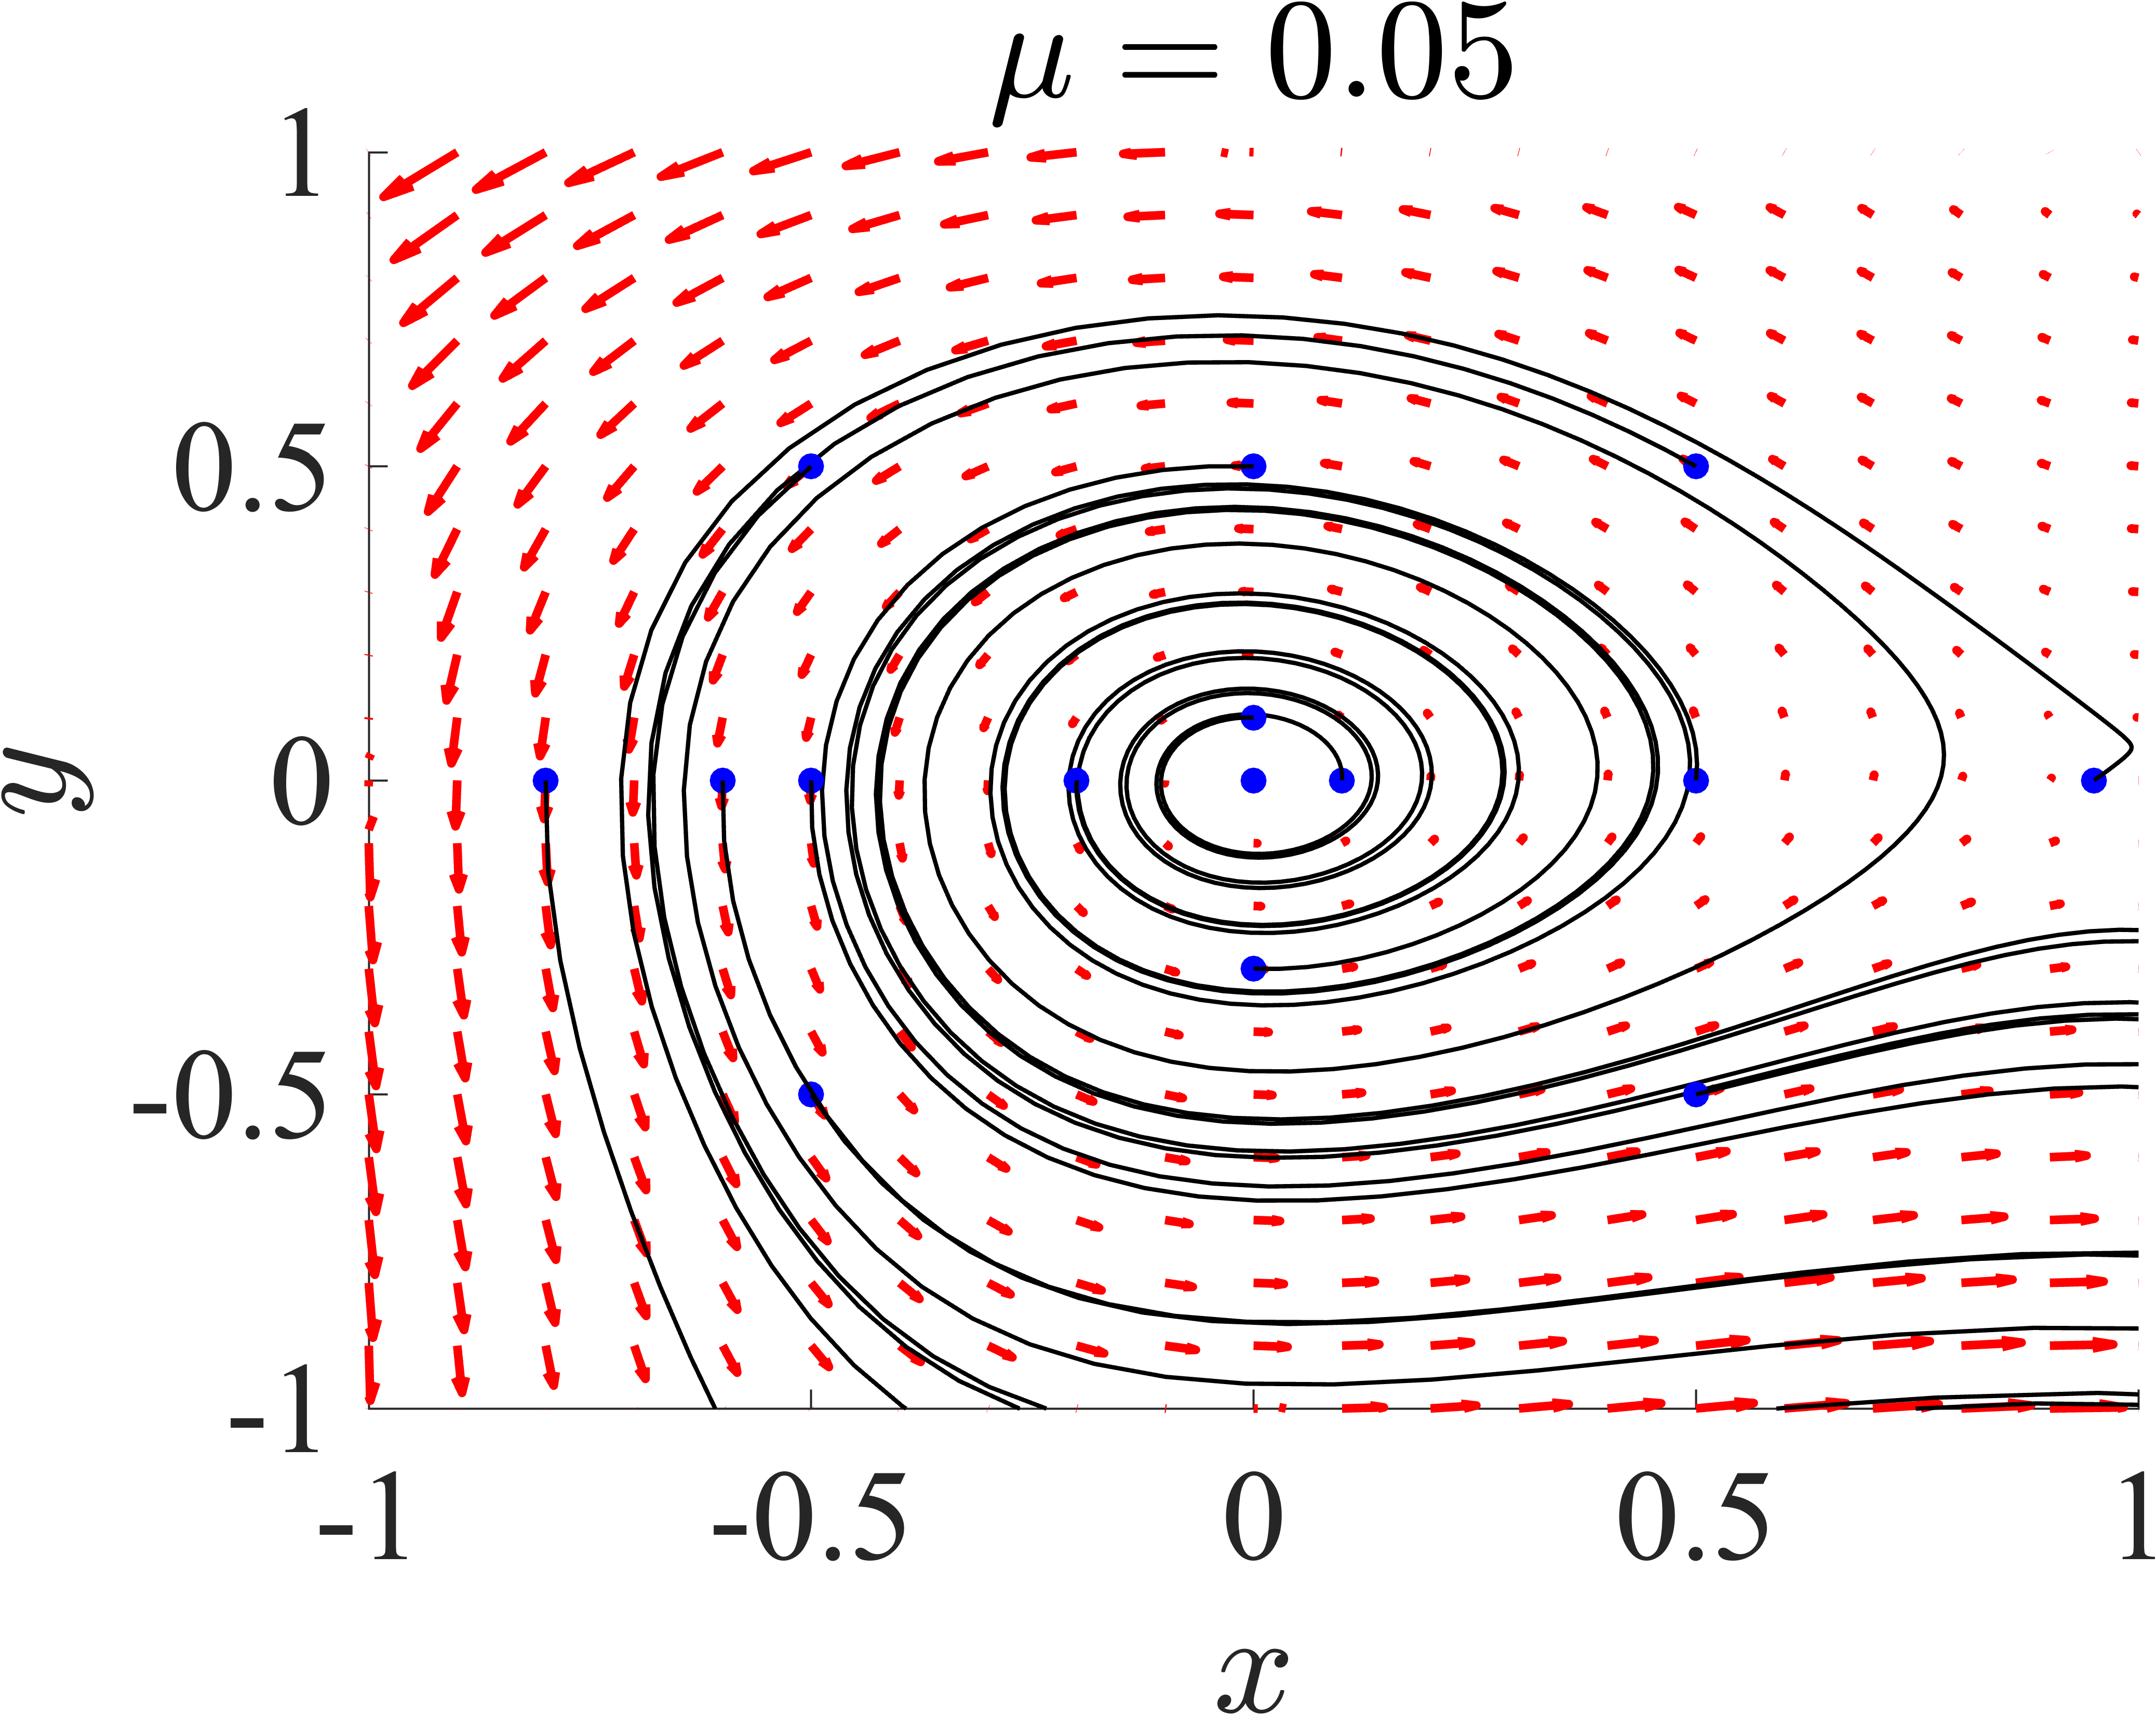
\includegraphics[width=7cm]{Hopf_823_phase_mu0.05.png}
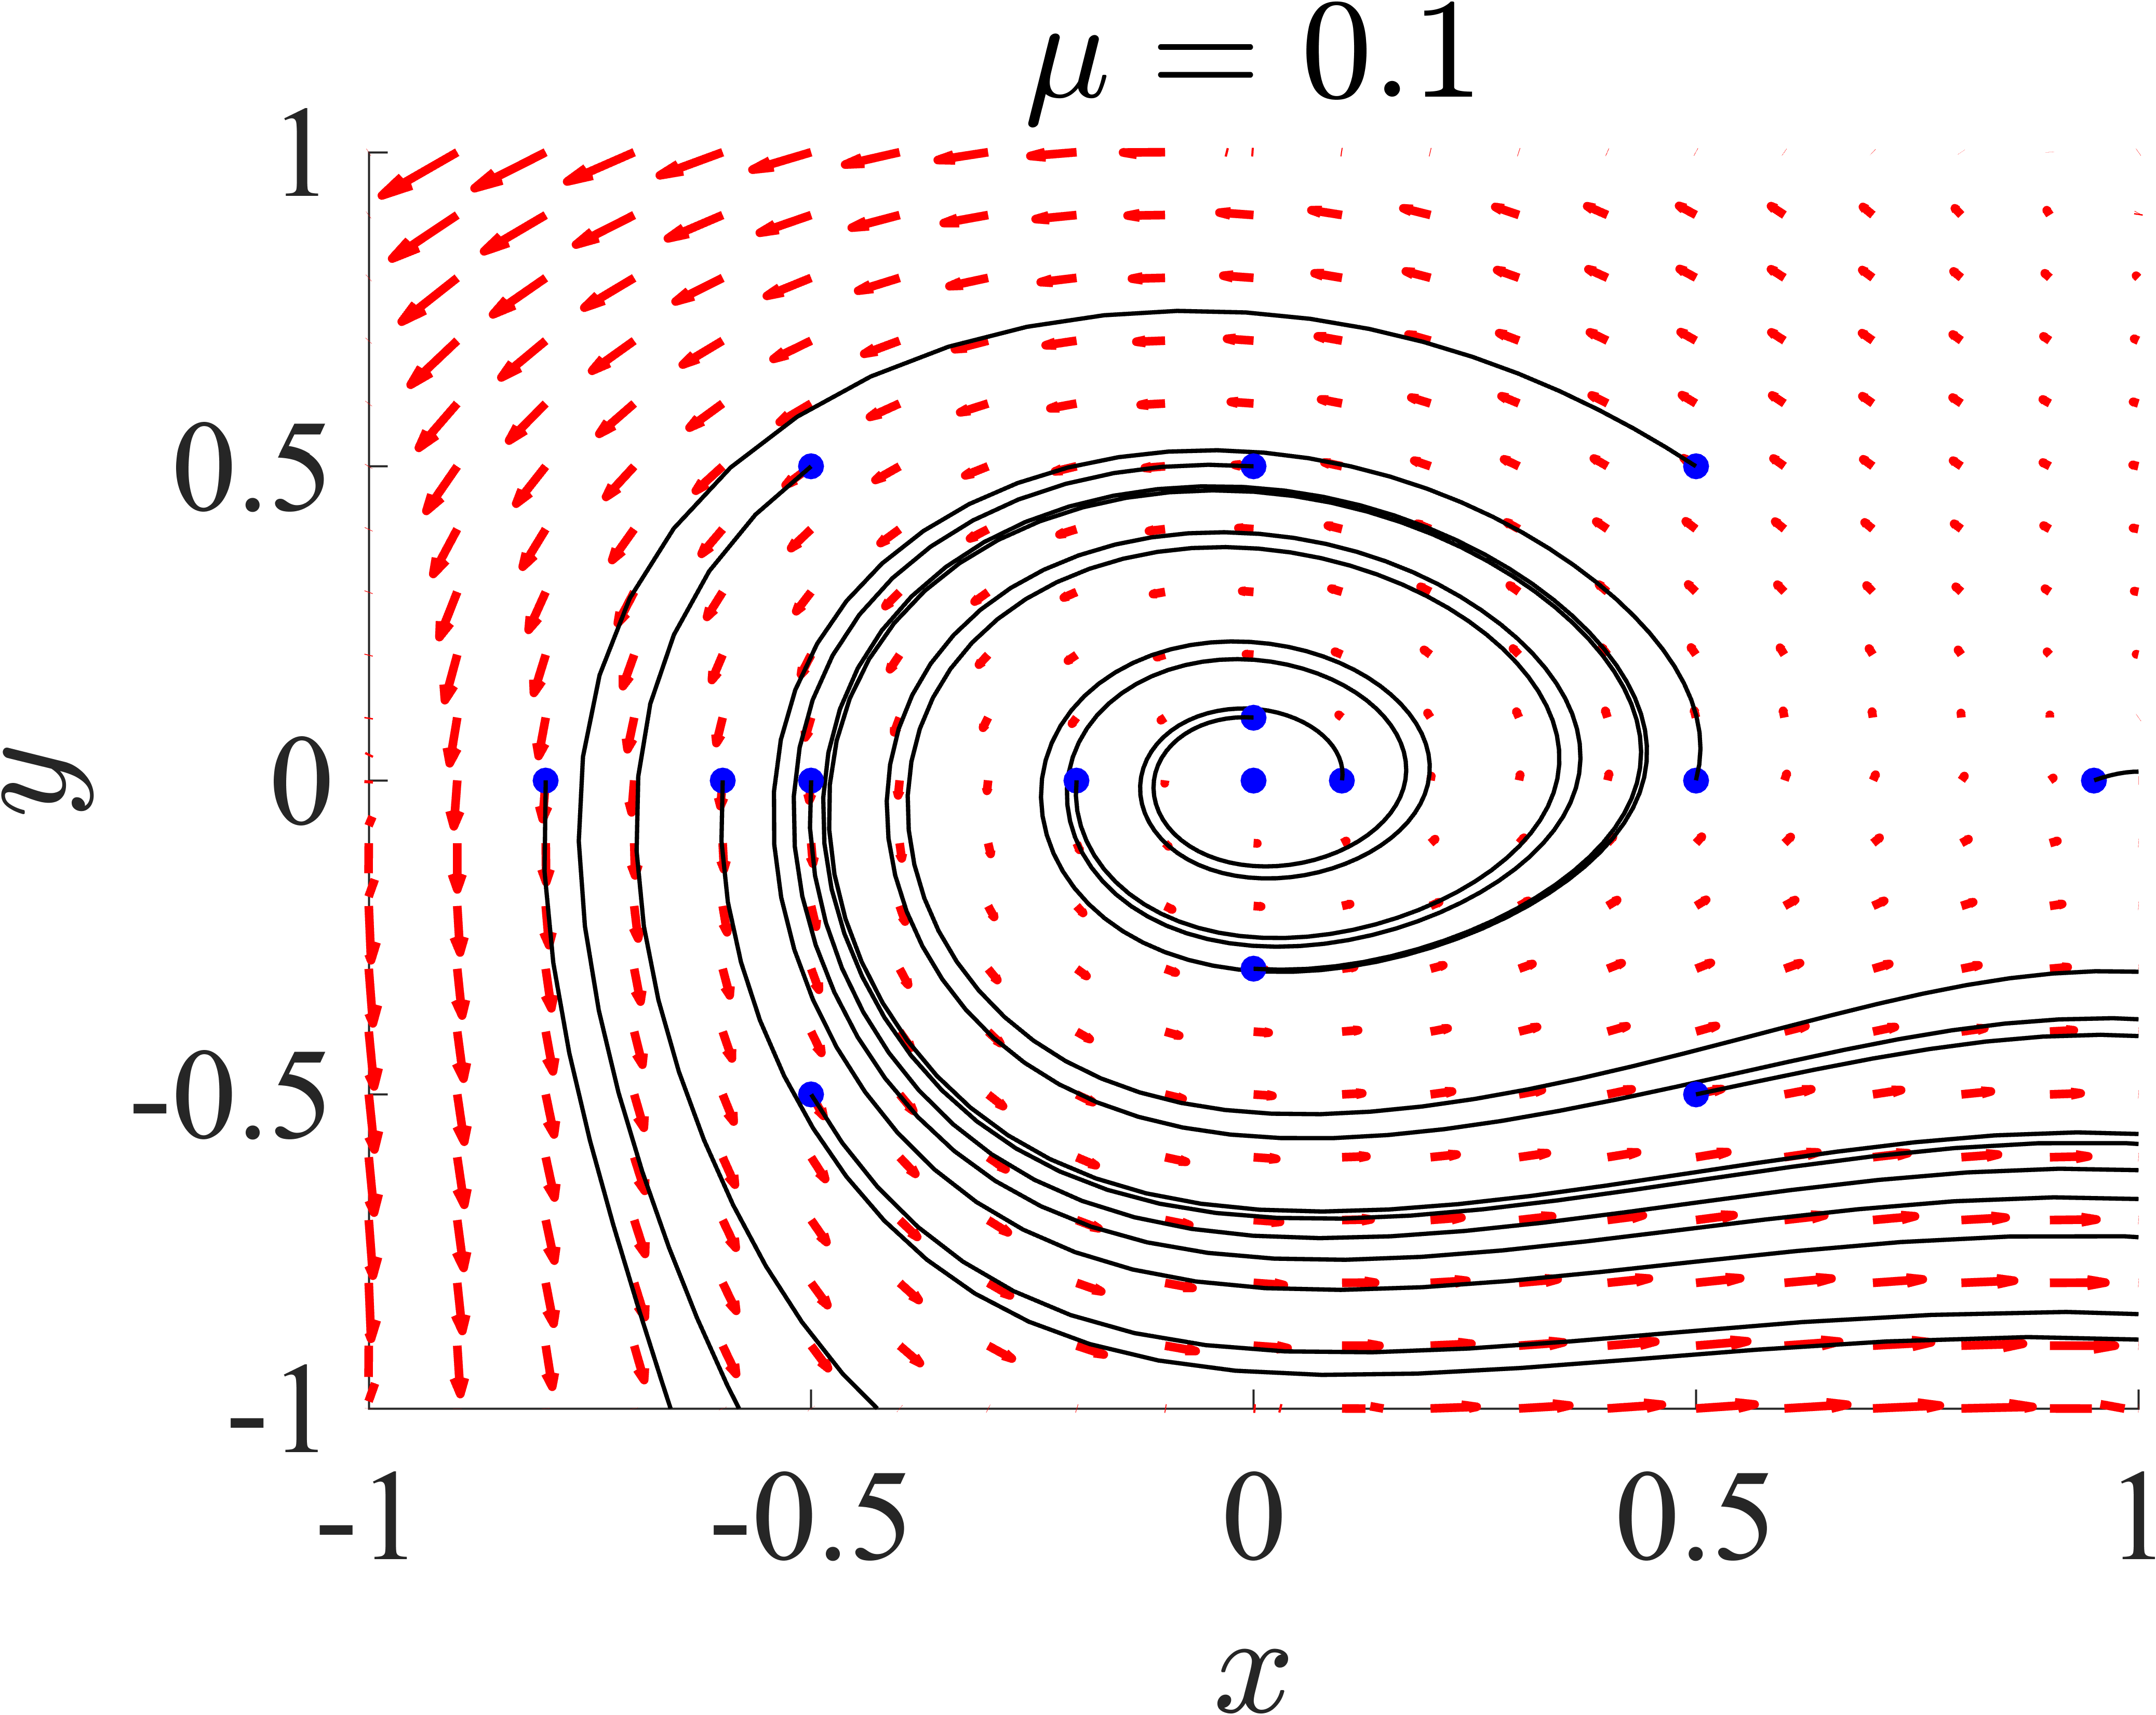
\includegraphics[width=7cm]{Hopf_823_phase_mu0.1.png}
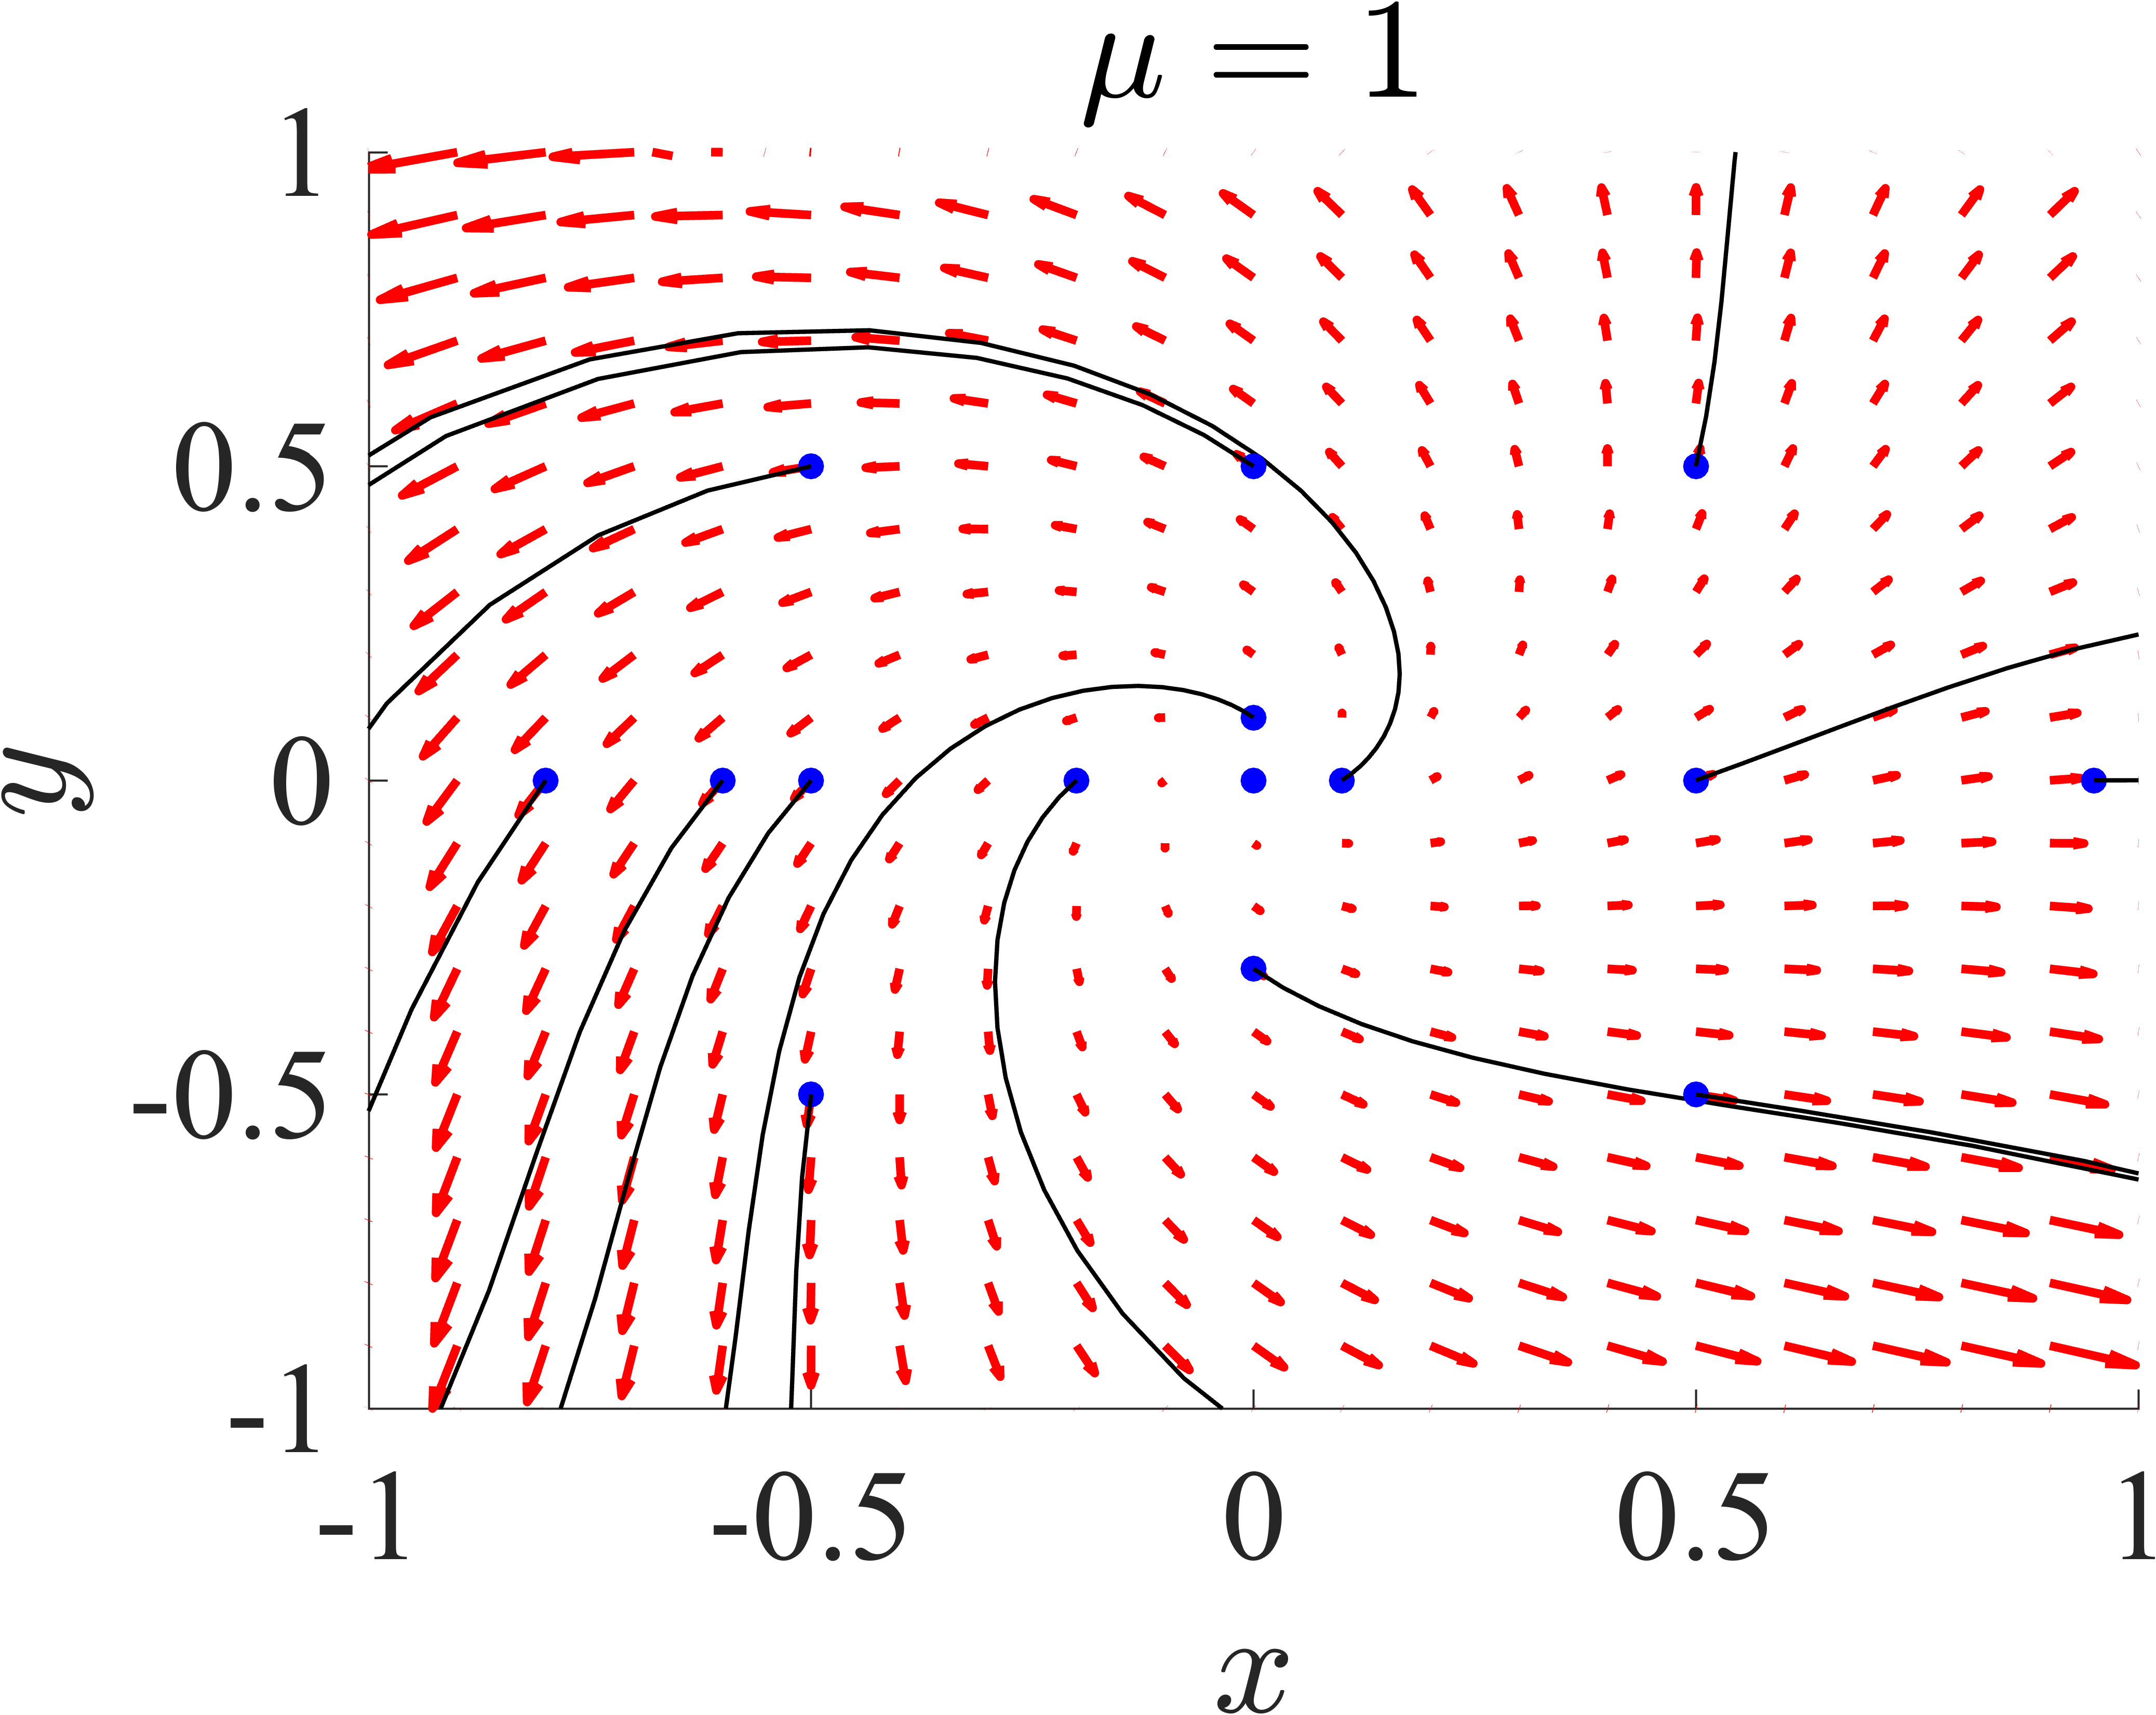
\includegraphics[width=7cm]{Hopf_823_phase_mu1.png}
\caption{Phase Portrait for $\mu > 0$}
\end{figure}
\clearpage

\section*{Problem 8.2.4.c}
Here, I plotted the phase portrait and numerically computed solutions for the approximated polar equation $\dot \theta \approx 1$ and $\dot r \approx \mu r + \frac{1}{8} r^3$. Initial conditions are shown as blue dots. A circle of radius $r = \sqrt{-8 \mu}$ is shown in green. Thus, we see that this circle represents an unstable limit cycle with the predicted radius of $r = \sqrt{-8 \mu}$, which confirms our prediction made by finding the radius at which $\dot r$ switches signs. I did this in MATLAB and converted between polar and cartesian coordinates as appropriate.

\begin{figure}[h]
\centering
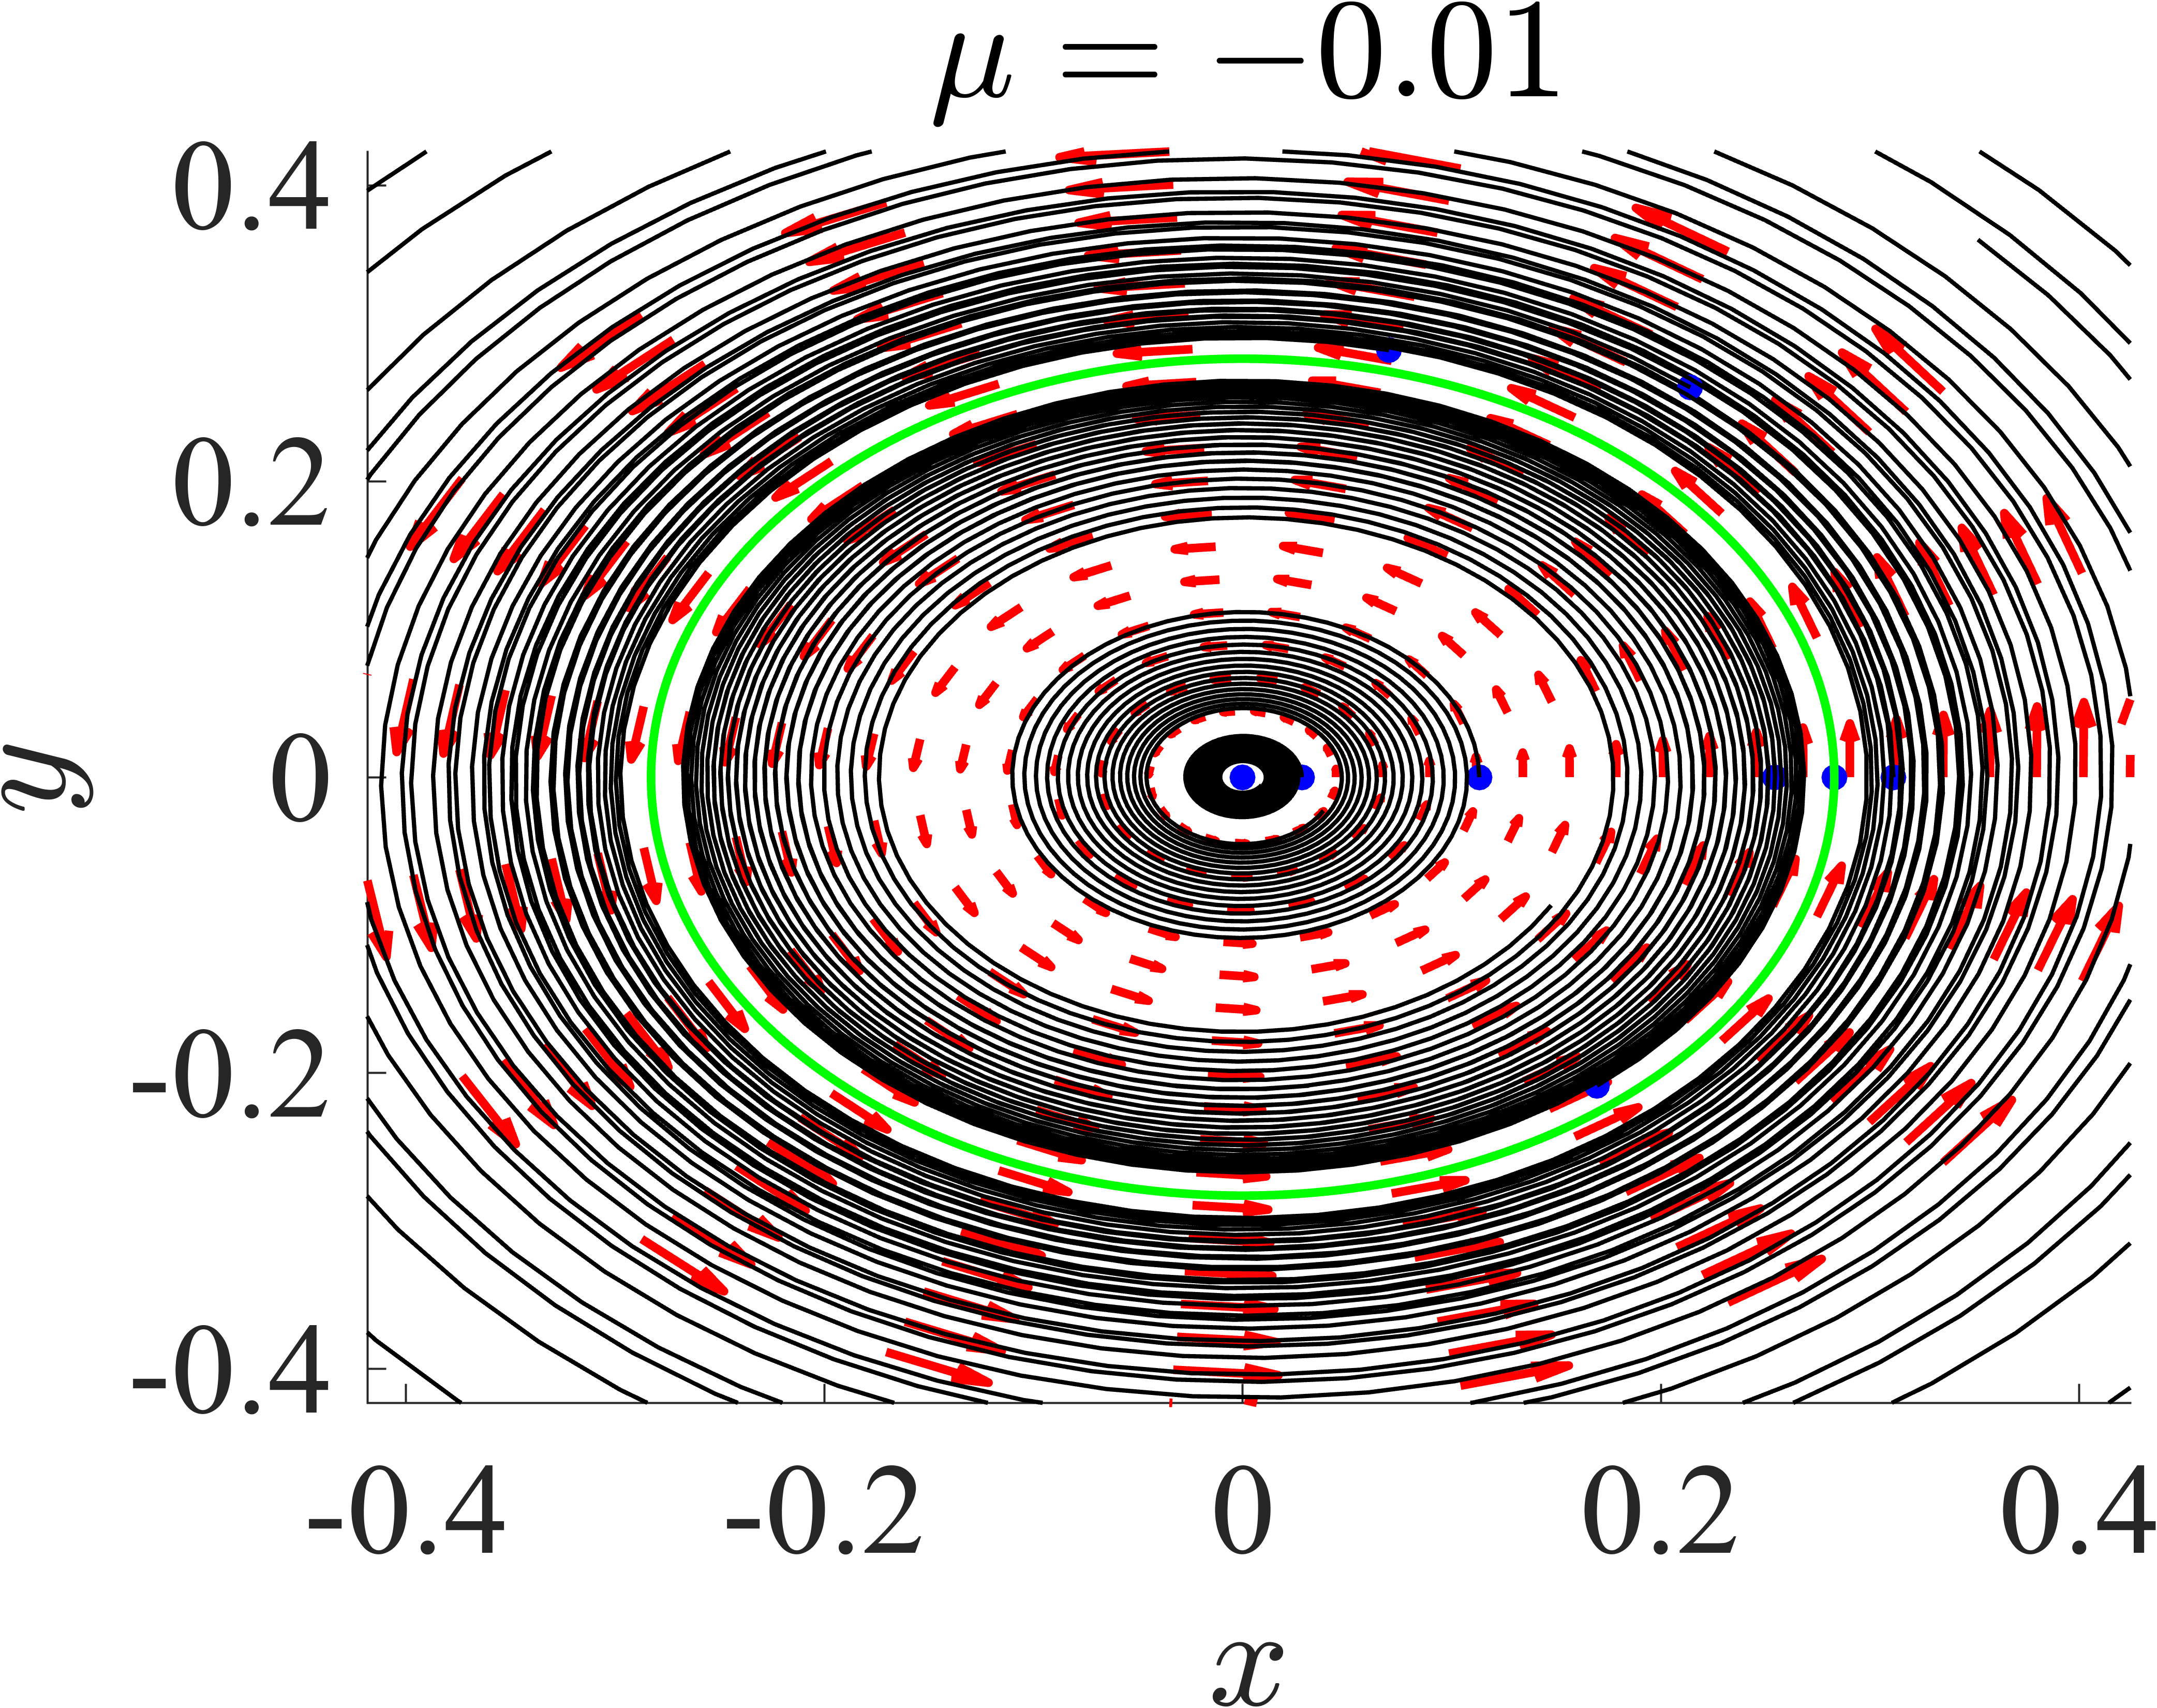
\includegraphics[width=8cm]{Heuristic_824.png}
\caption{Phase Portrait for Approximated Polar Representation of System}
\end{figure}
\clearpage

\section*{Problem 8.2.11b}
I plotted the phase portraits for $\mu > 0$, $\mu = 0$, and $\mu < 0$, shown below. We see here that when $\mu < 0$, the fixed point at the origin is unstable (an unstable spiral), as we previously saw. When $\mu > 0$, the fixed point at the origin is a stable spiral. However, at $\mu = 0$, we have a continuous band of closed orbits surrounding the origin, not limit cycles (which are isolated closed orbit). Thus, we have a degenerate Hopf bifurcation. 

\begin{figure}[h]
\centering
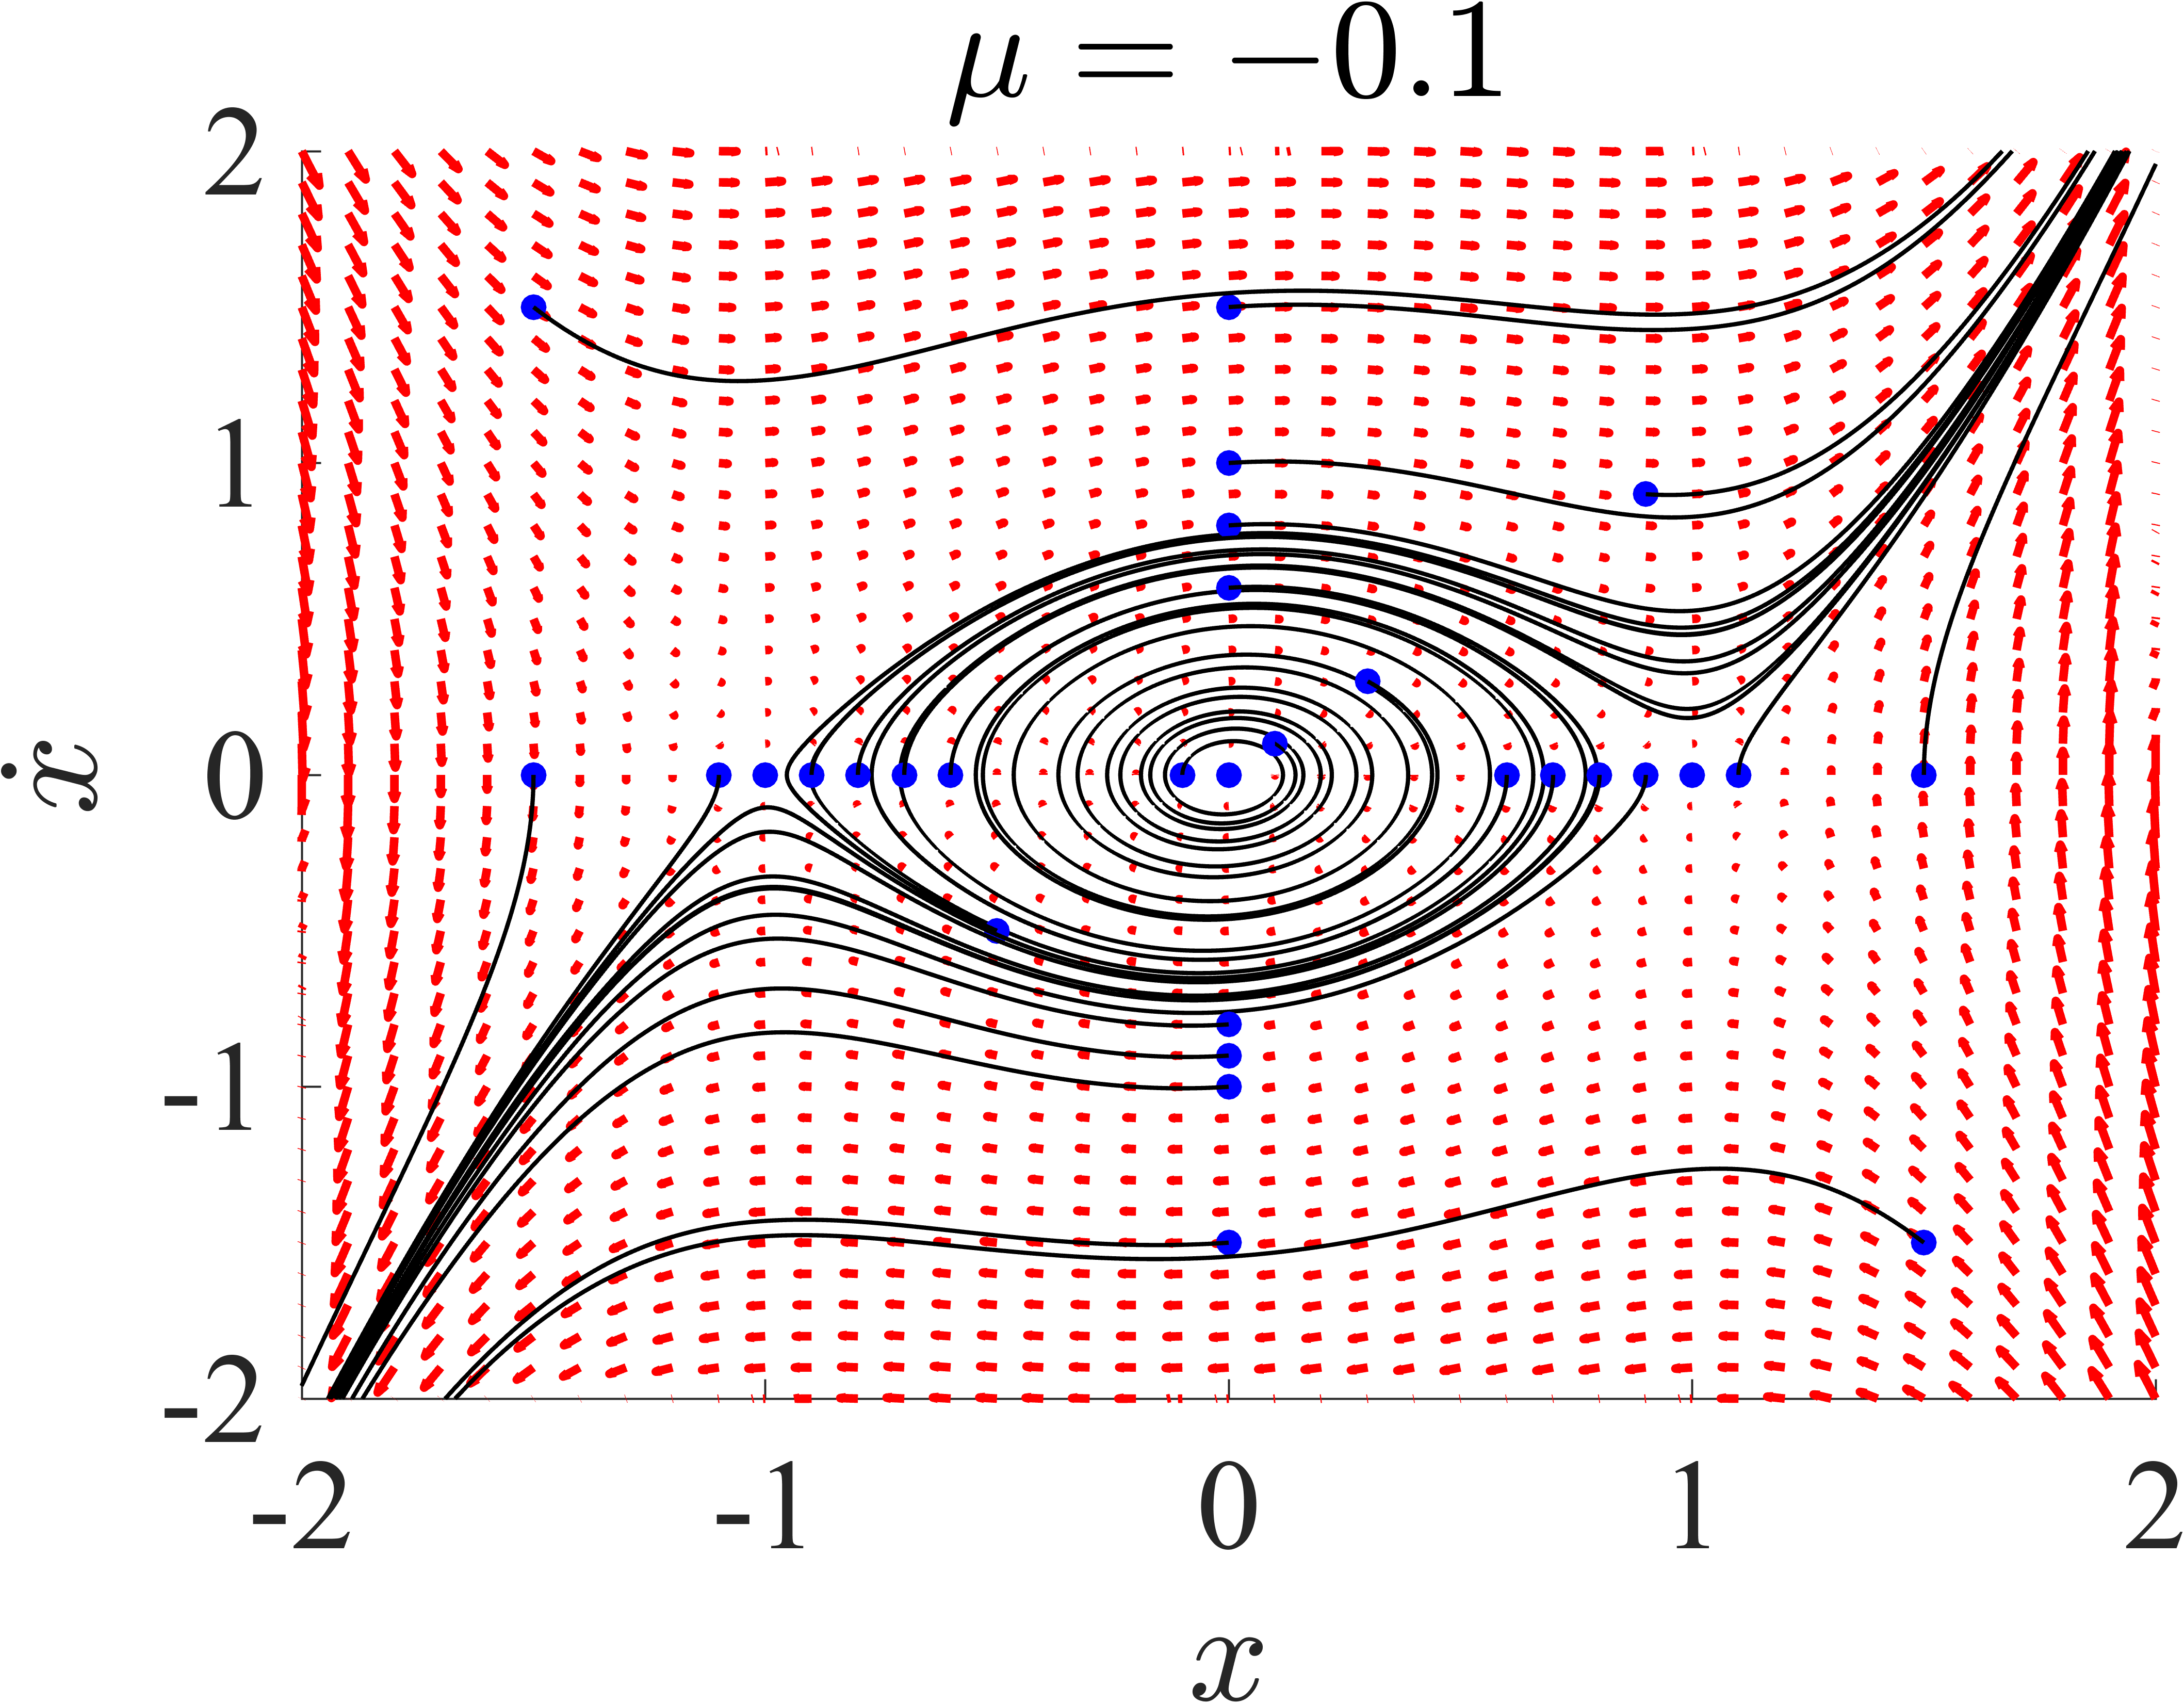
\includegraphics[width=8cm]{PhasePlot_8211_-0.1.png}
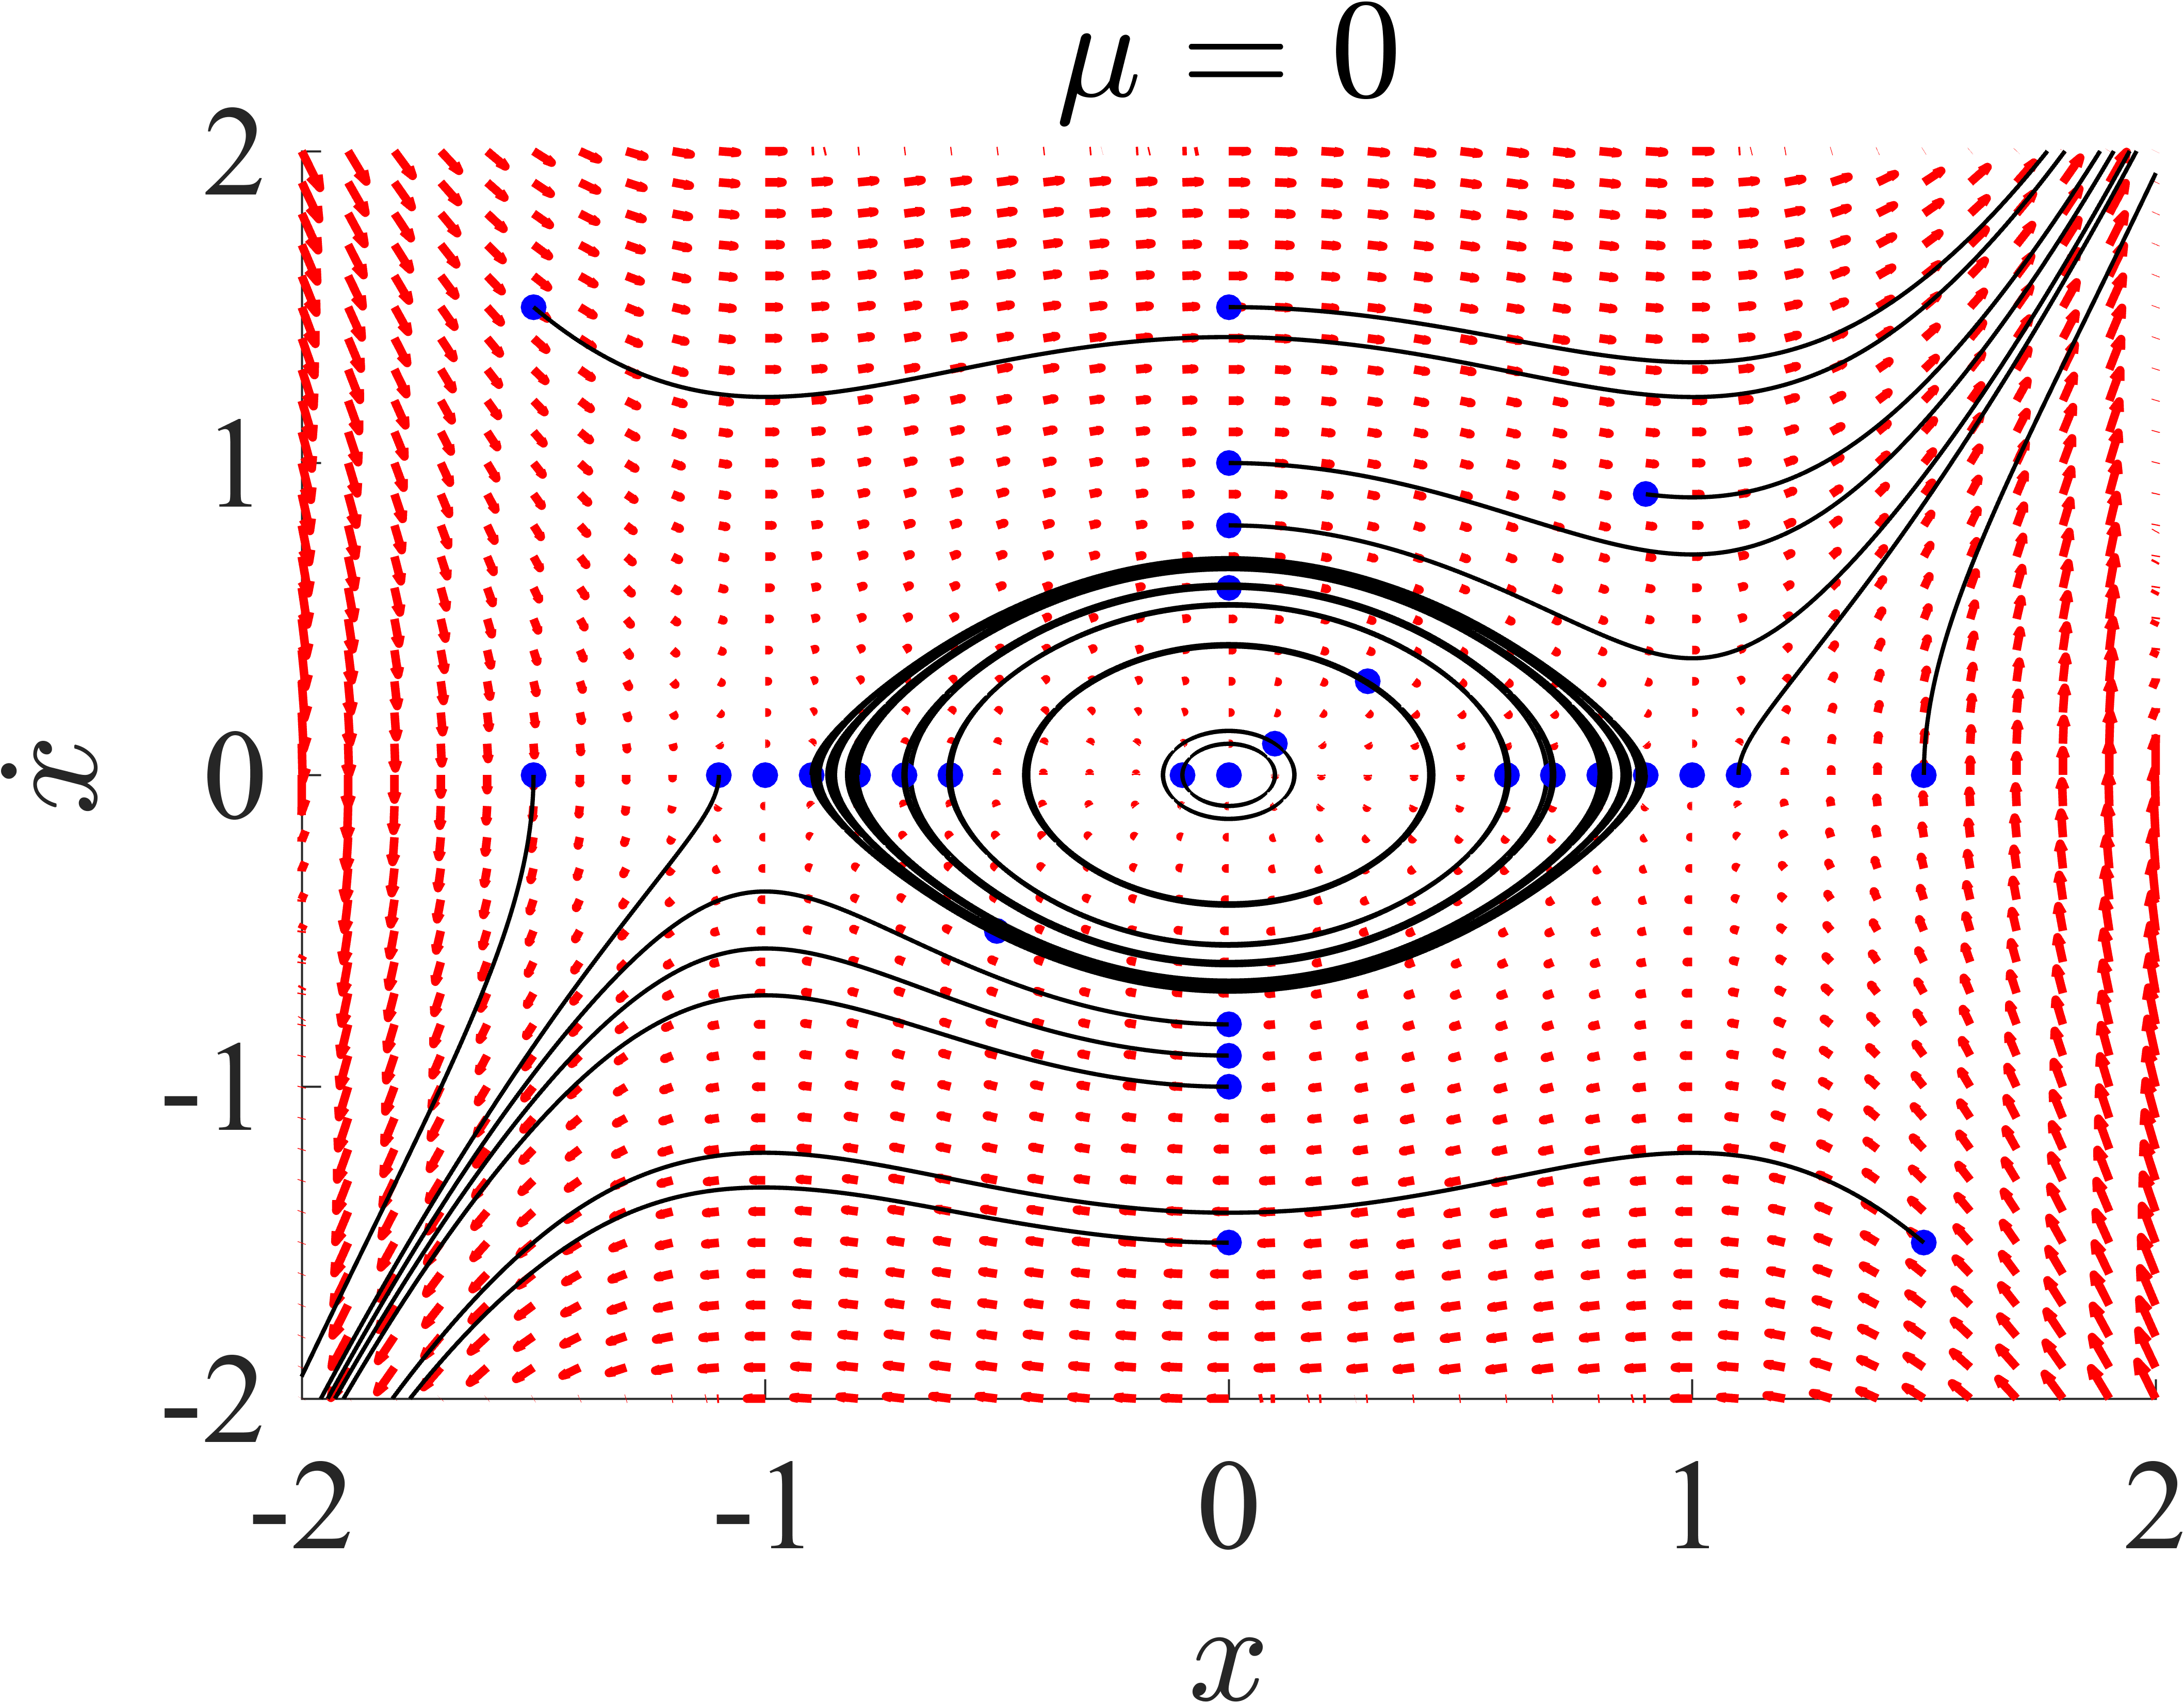
\includegraphics[width=8cm]{PhasePlot_8211_0.png}
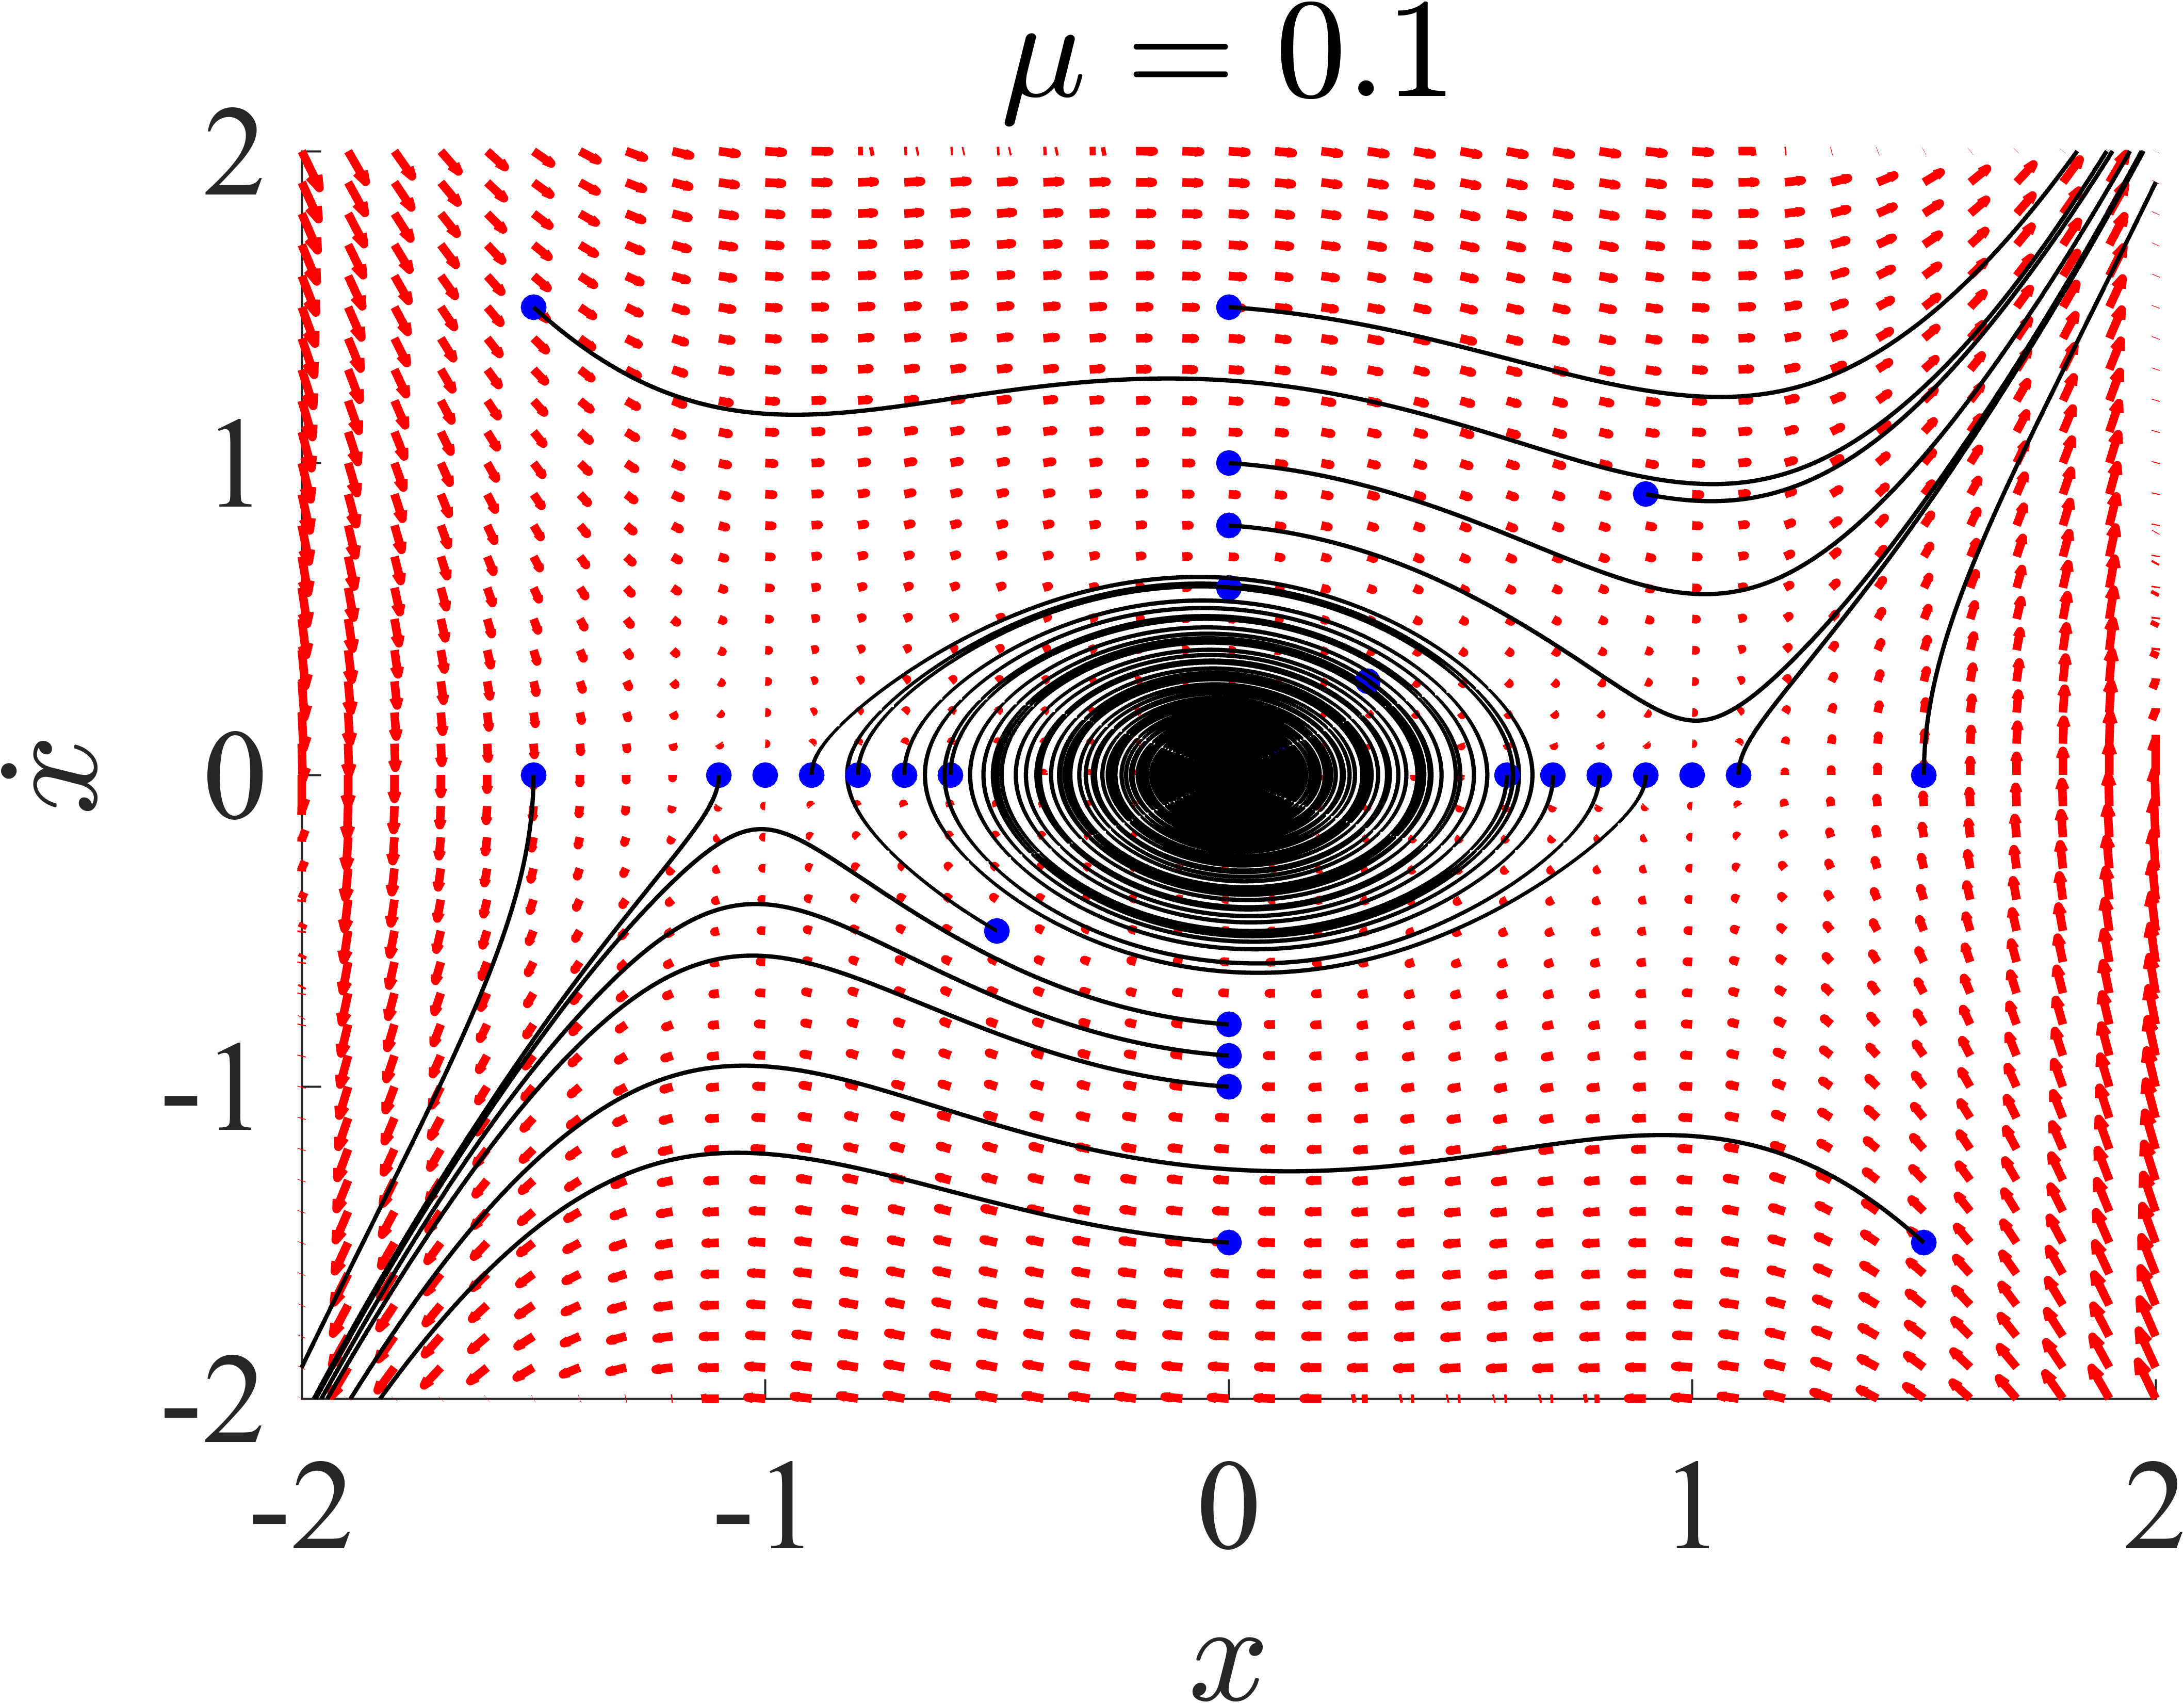
\includegraphics[width=8cm]{PhasePlot_8211_0.1.png}
\caption{Phase Portraits for damped Duffing Oscillator}
\end{figure}


\section*{Problem 8.2.17e}
In this part, I show that the Hopf bifurcation (when the trace of $A - B$ is positive) can be supercritical. To simulate this, note that we have a four-variable system, so we can't plot the dynamics in all four variables. For this reason, I calculate the full ODE and solution trajectories and plot the resulting dynamics of the variables that we are most interested in, which are the activity levels of the two populations of neurons ($x_1$ and $x_2$). So when we do this, I plot a phase plane at constant $y_1$ and $y_2$ values. I solve my ODE with $y_0$, or the initial state of the system, being at the $y_1$ and $y_2$ values of the phase plot. I also start my system at $x_1 \neq x_2$ and $y_1 \neq y_2$. Note that when the trajectories are plotted, we are seeing the projection onto the $x_1/x_2$ plane.

In the figures, I will also plot the initial conditions of trajectories as blue dots. I also plot the fixed point $u^*$, which is the point $u$ such that $u = F(I - u(b+g))$ (we determined this in part a of the problem), as a green dot. My results are shown below. 

\begin{figure}[h]
\centering
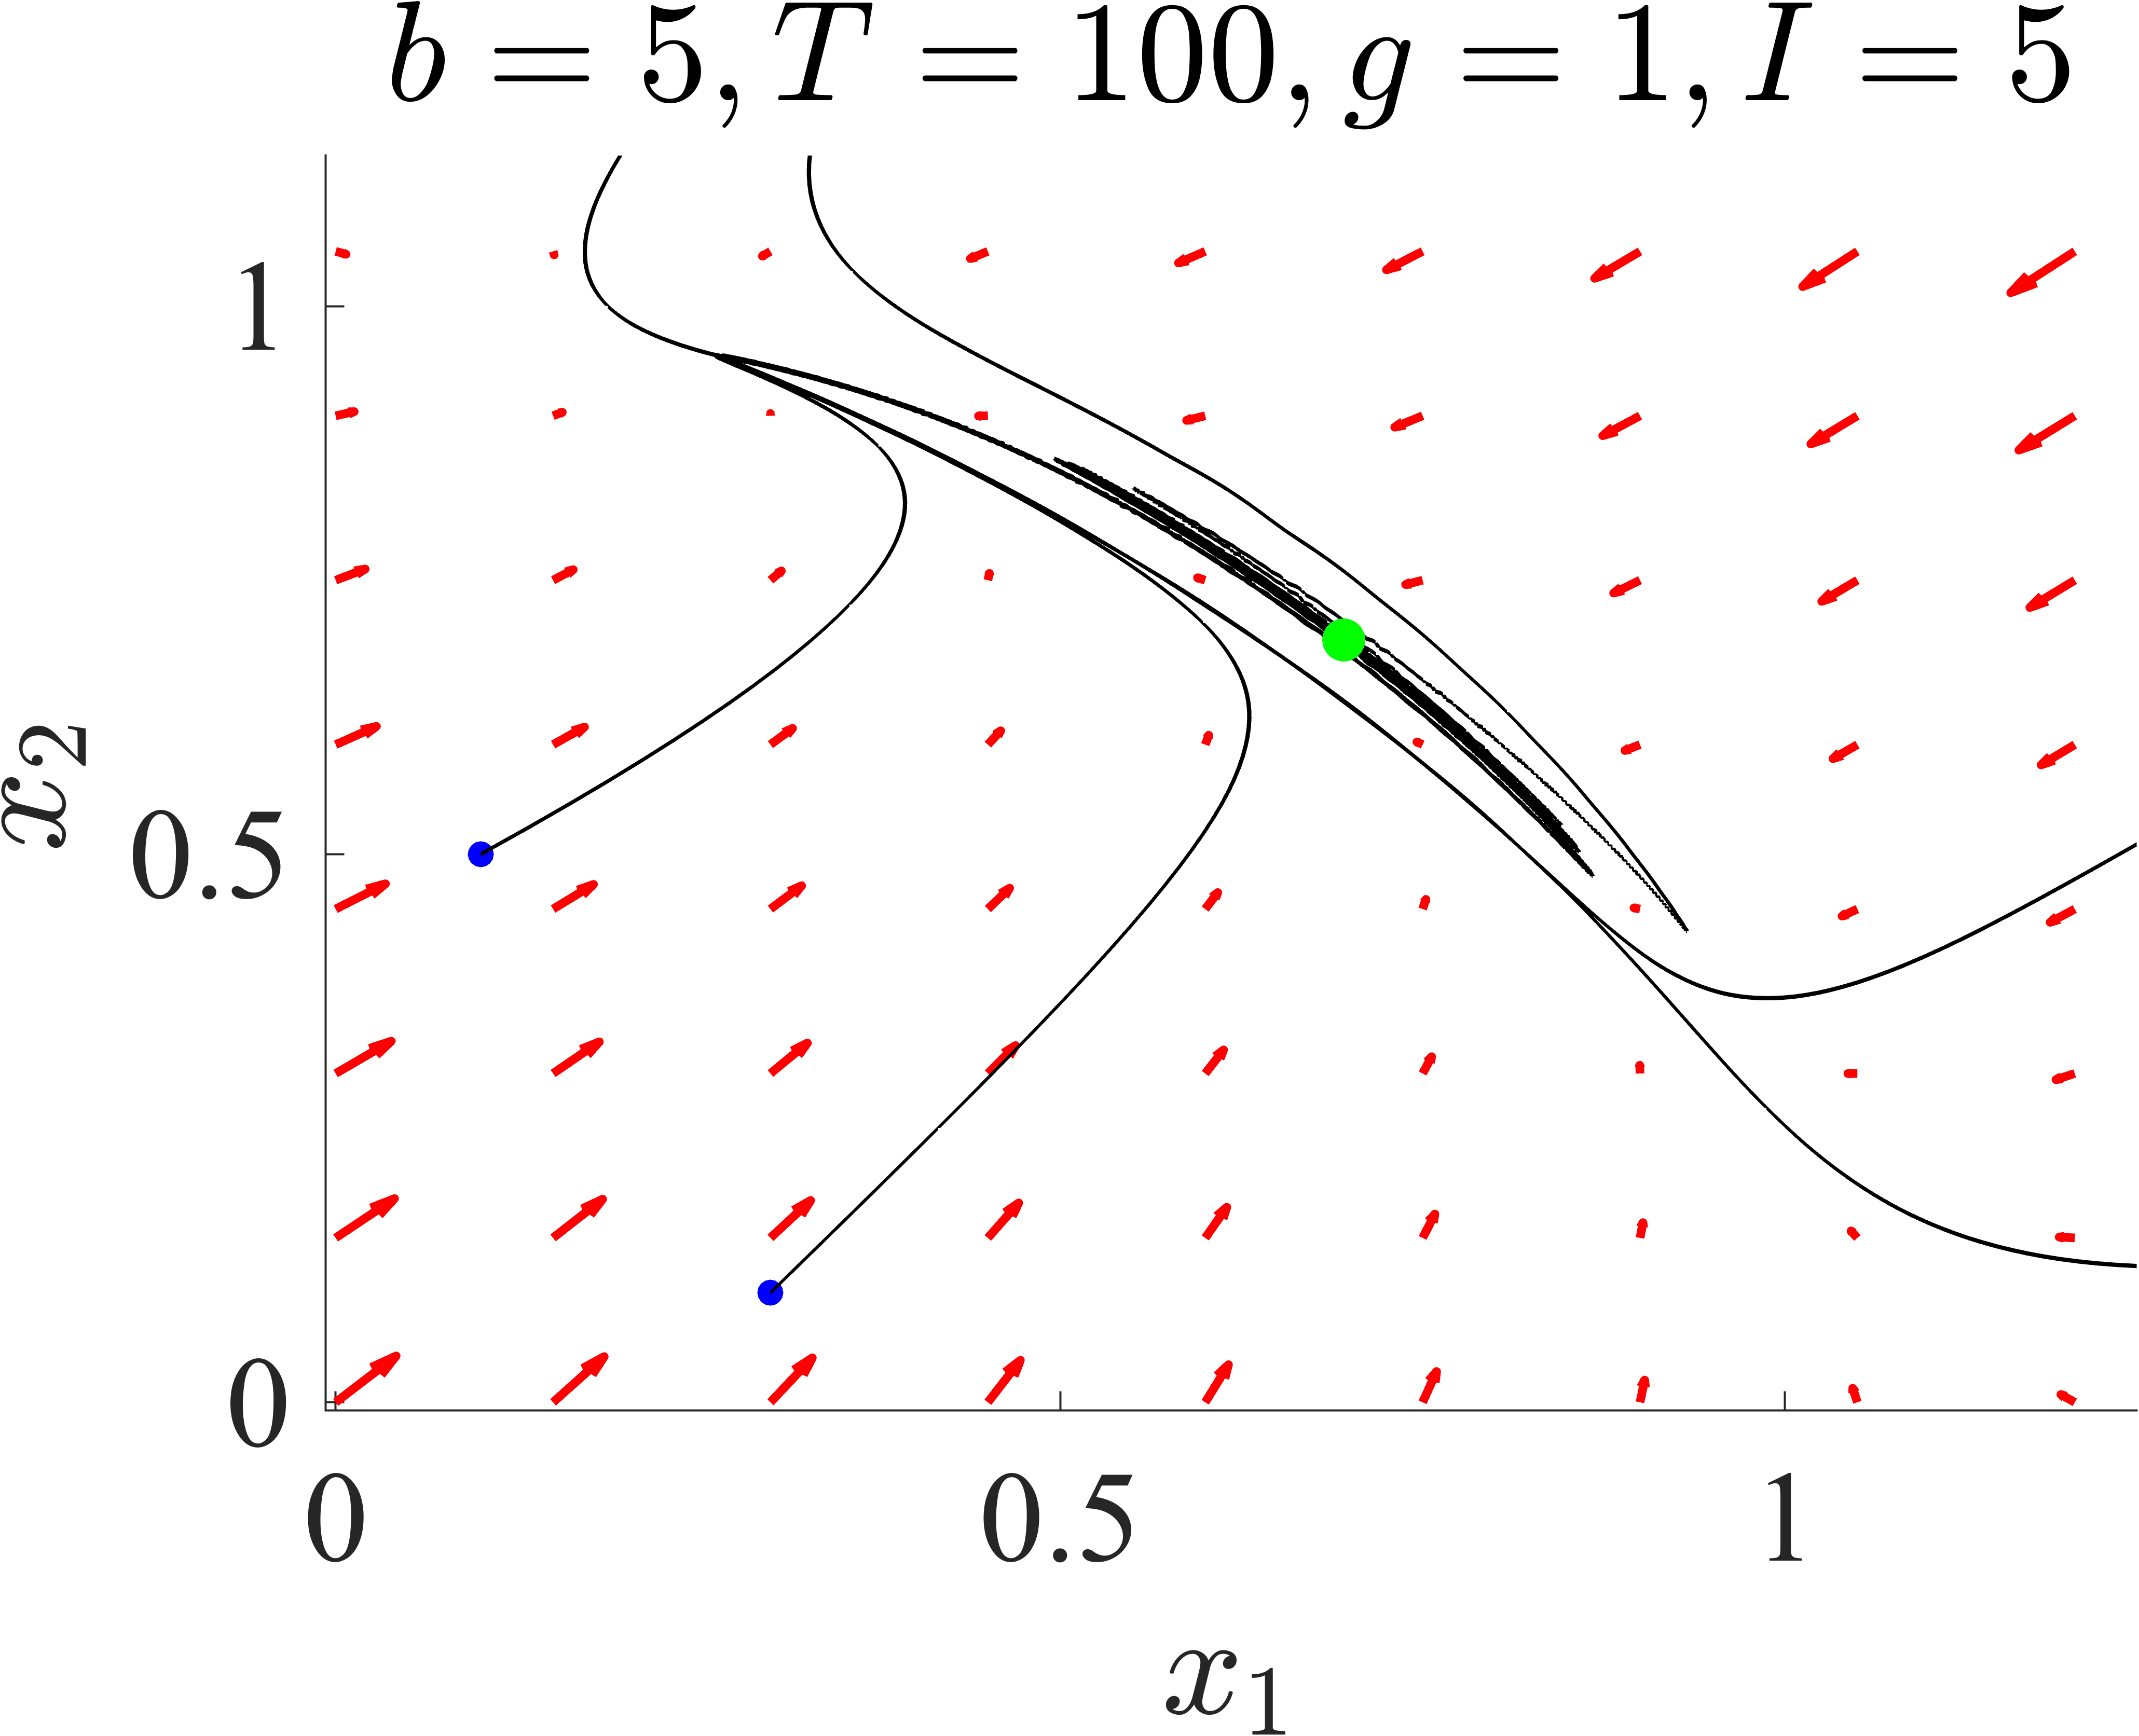
\includegraphics[width=8cm]{xs_HopfNeurons_b_5_T100_g1I_5_2.png}
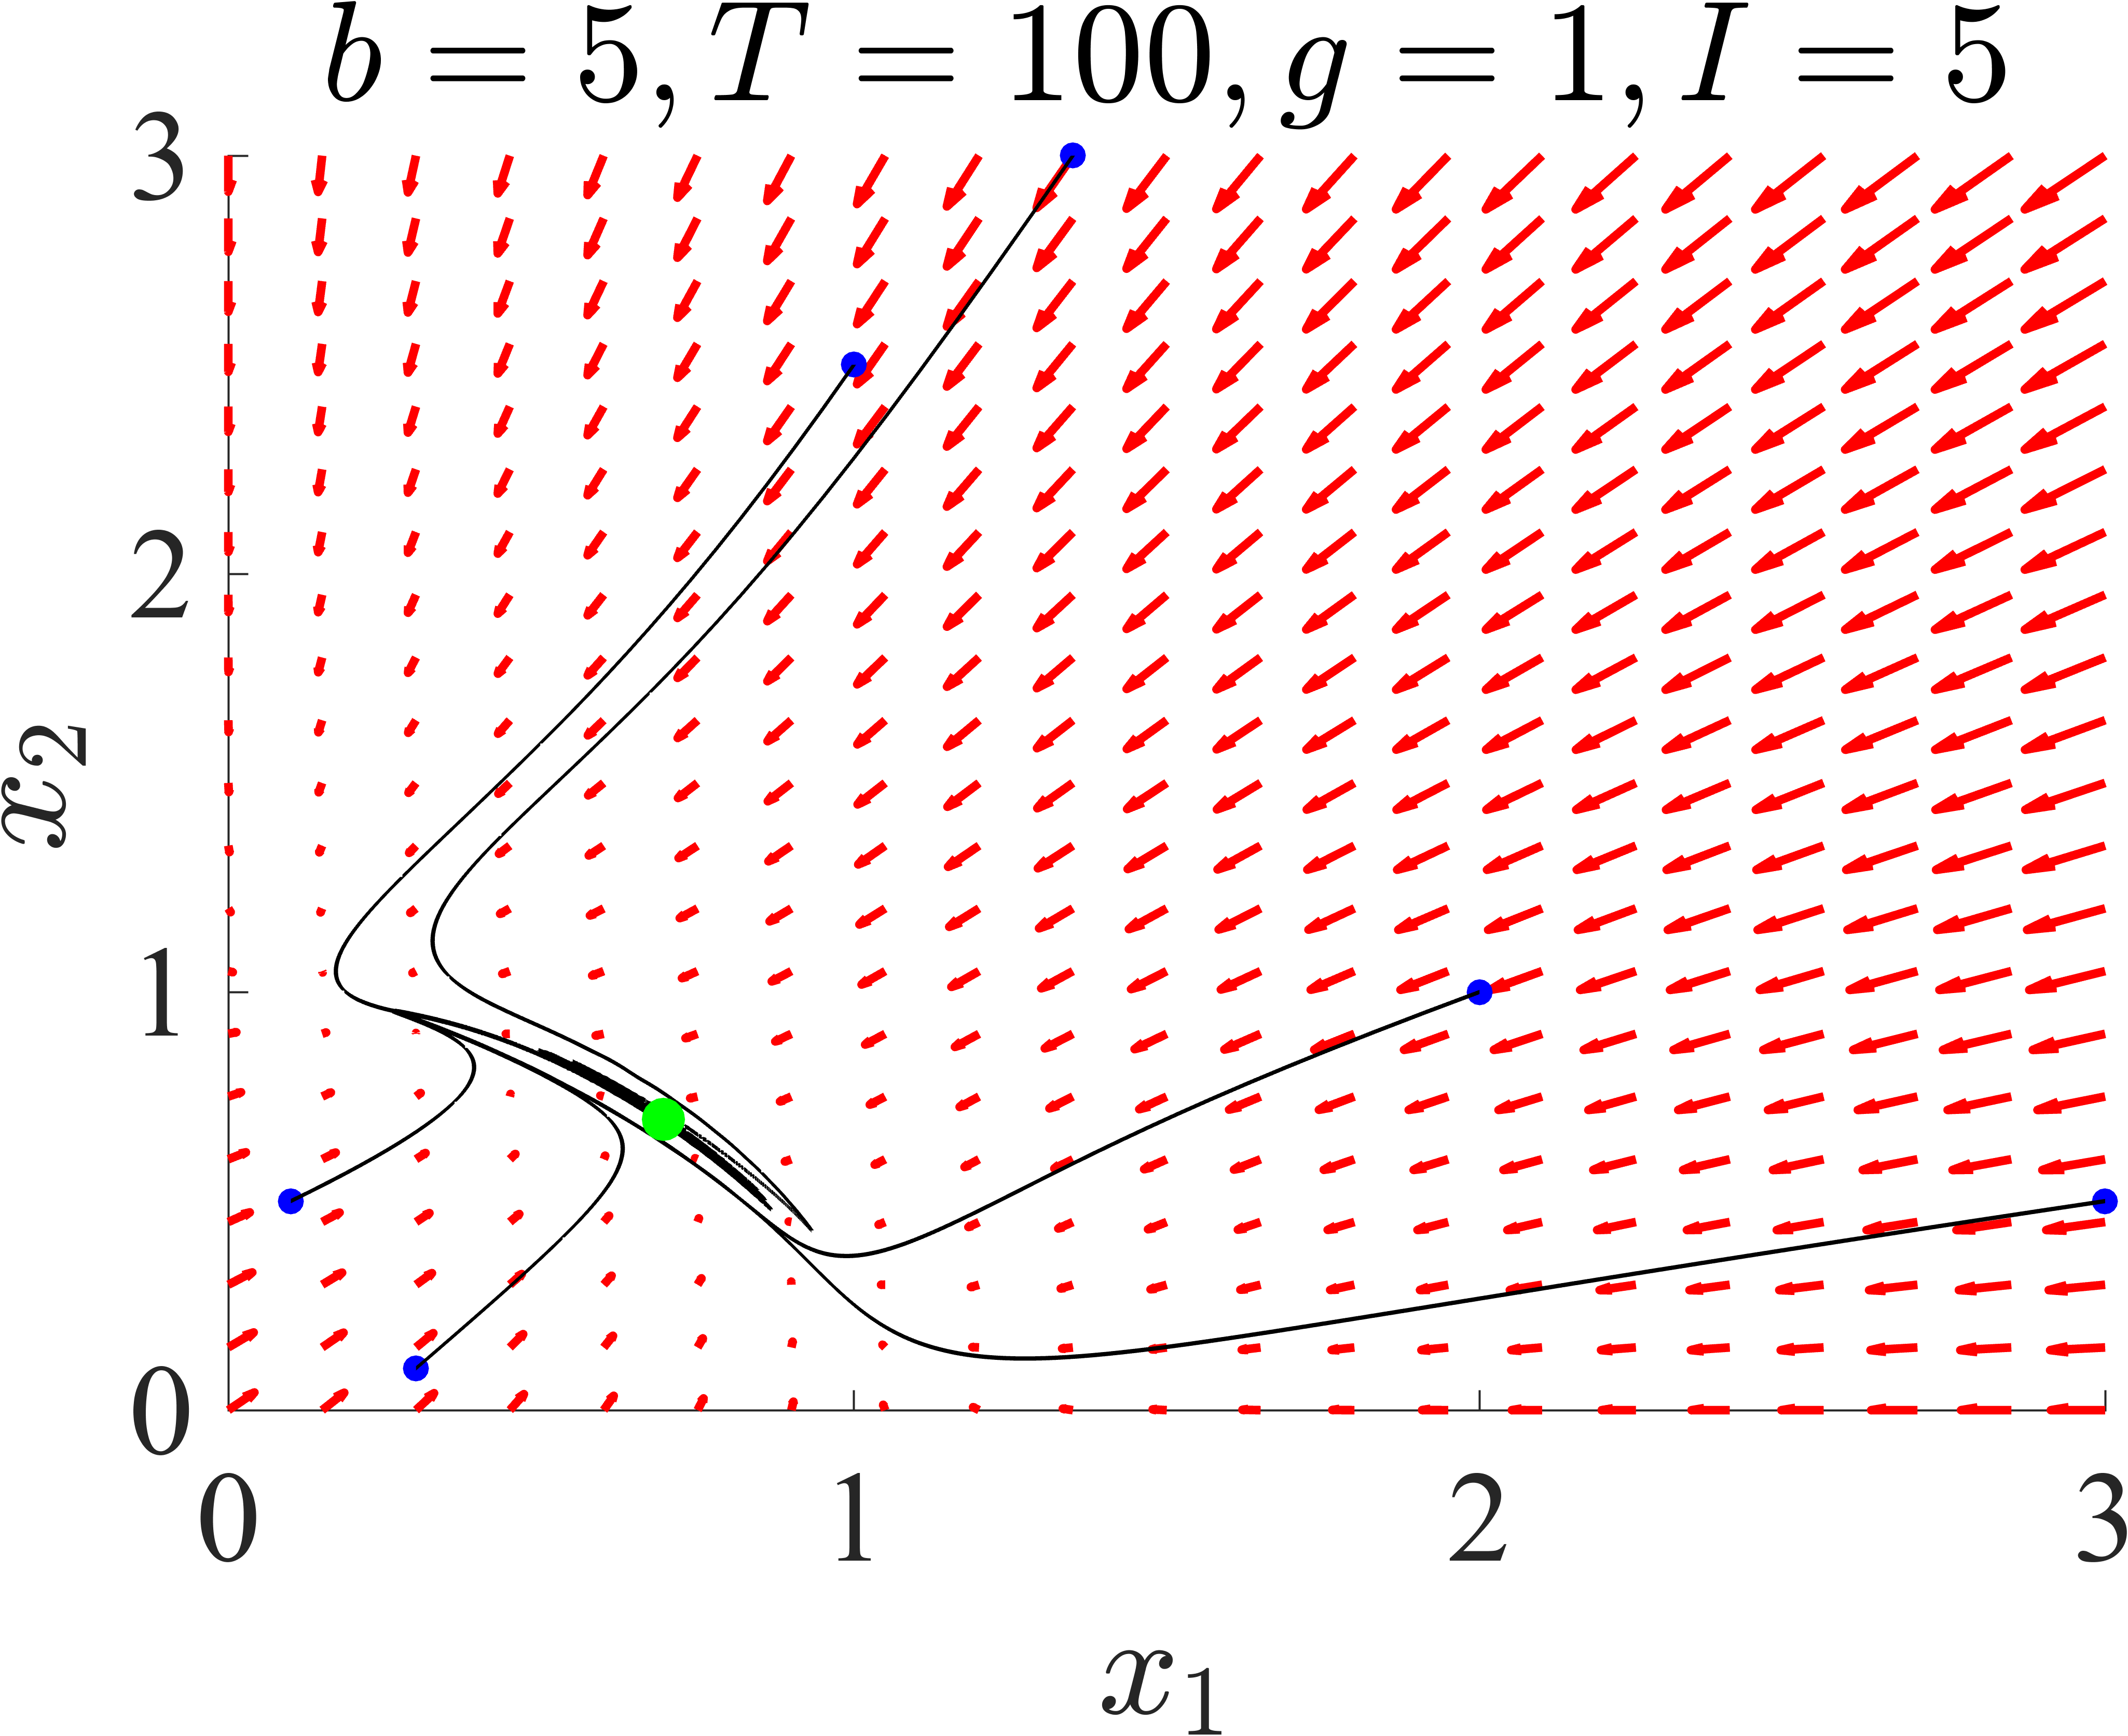
\includegraphics[width=8cm]{xs_HopfNeurons_b_5_T100_g1I_5.png}
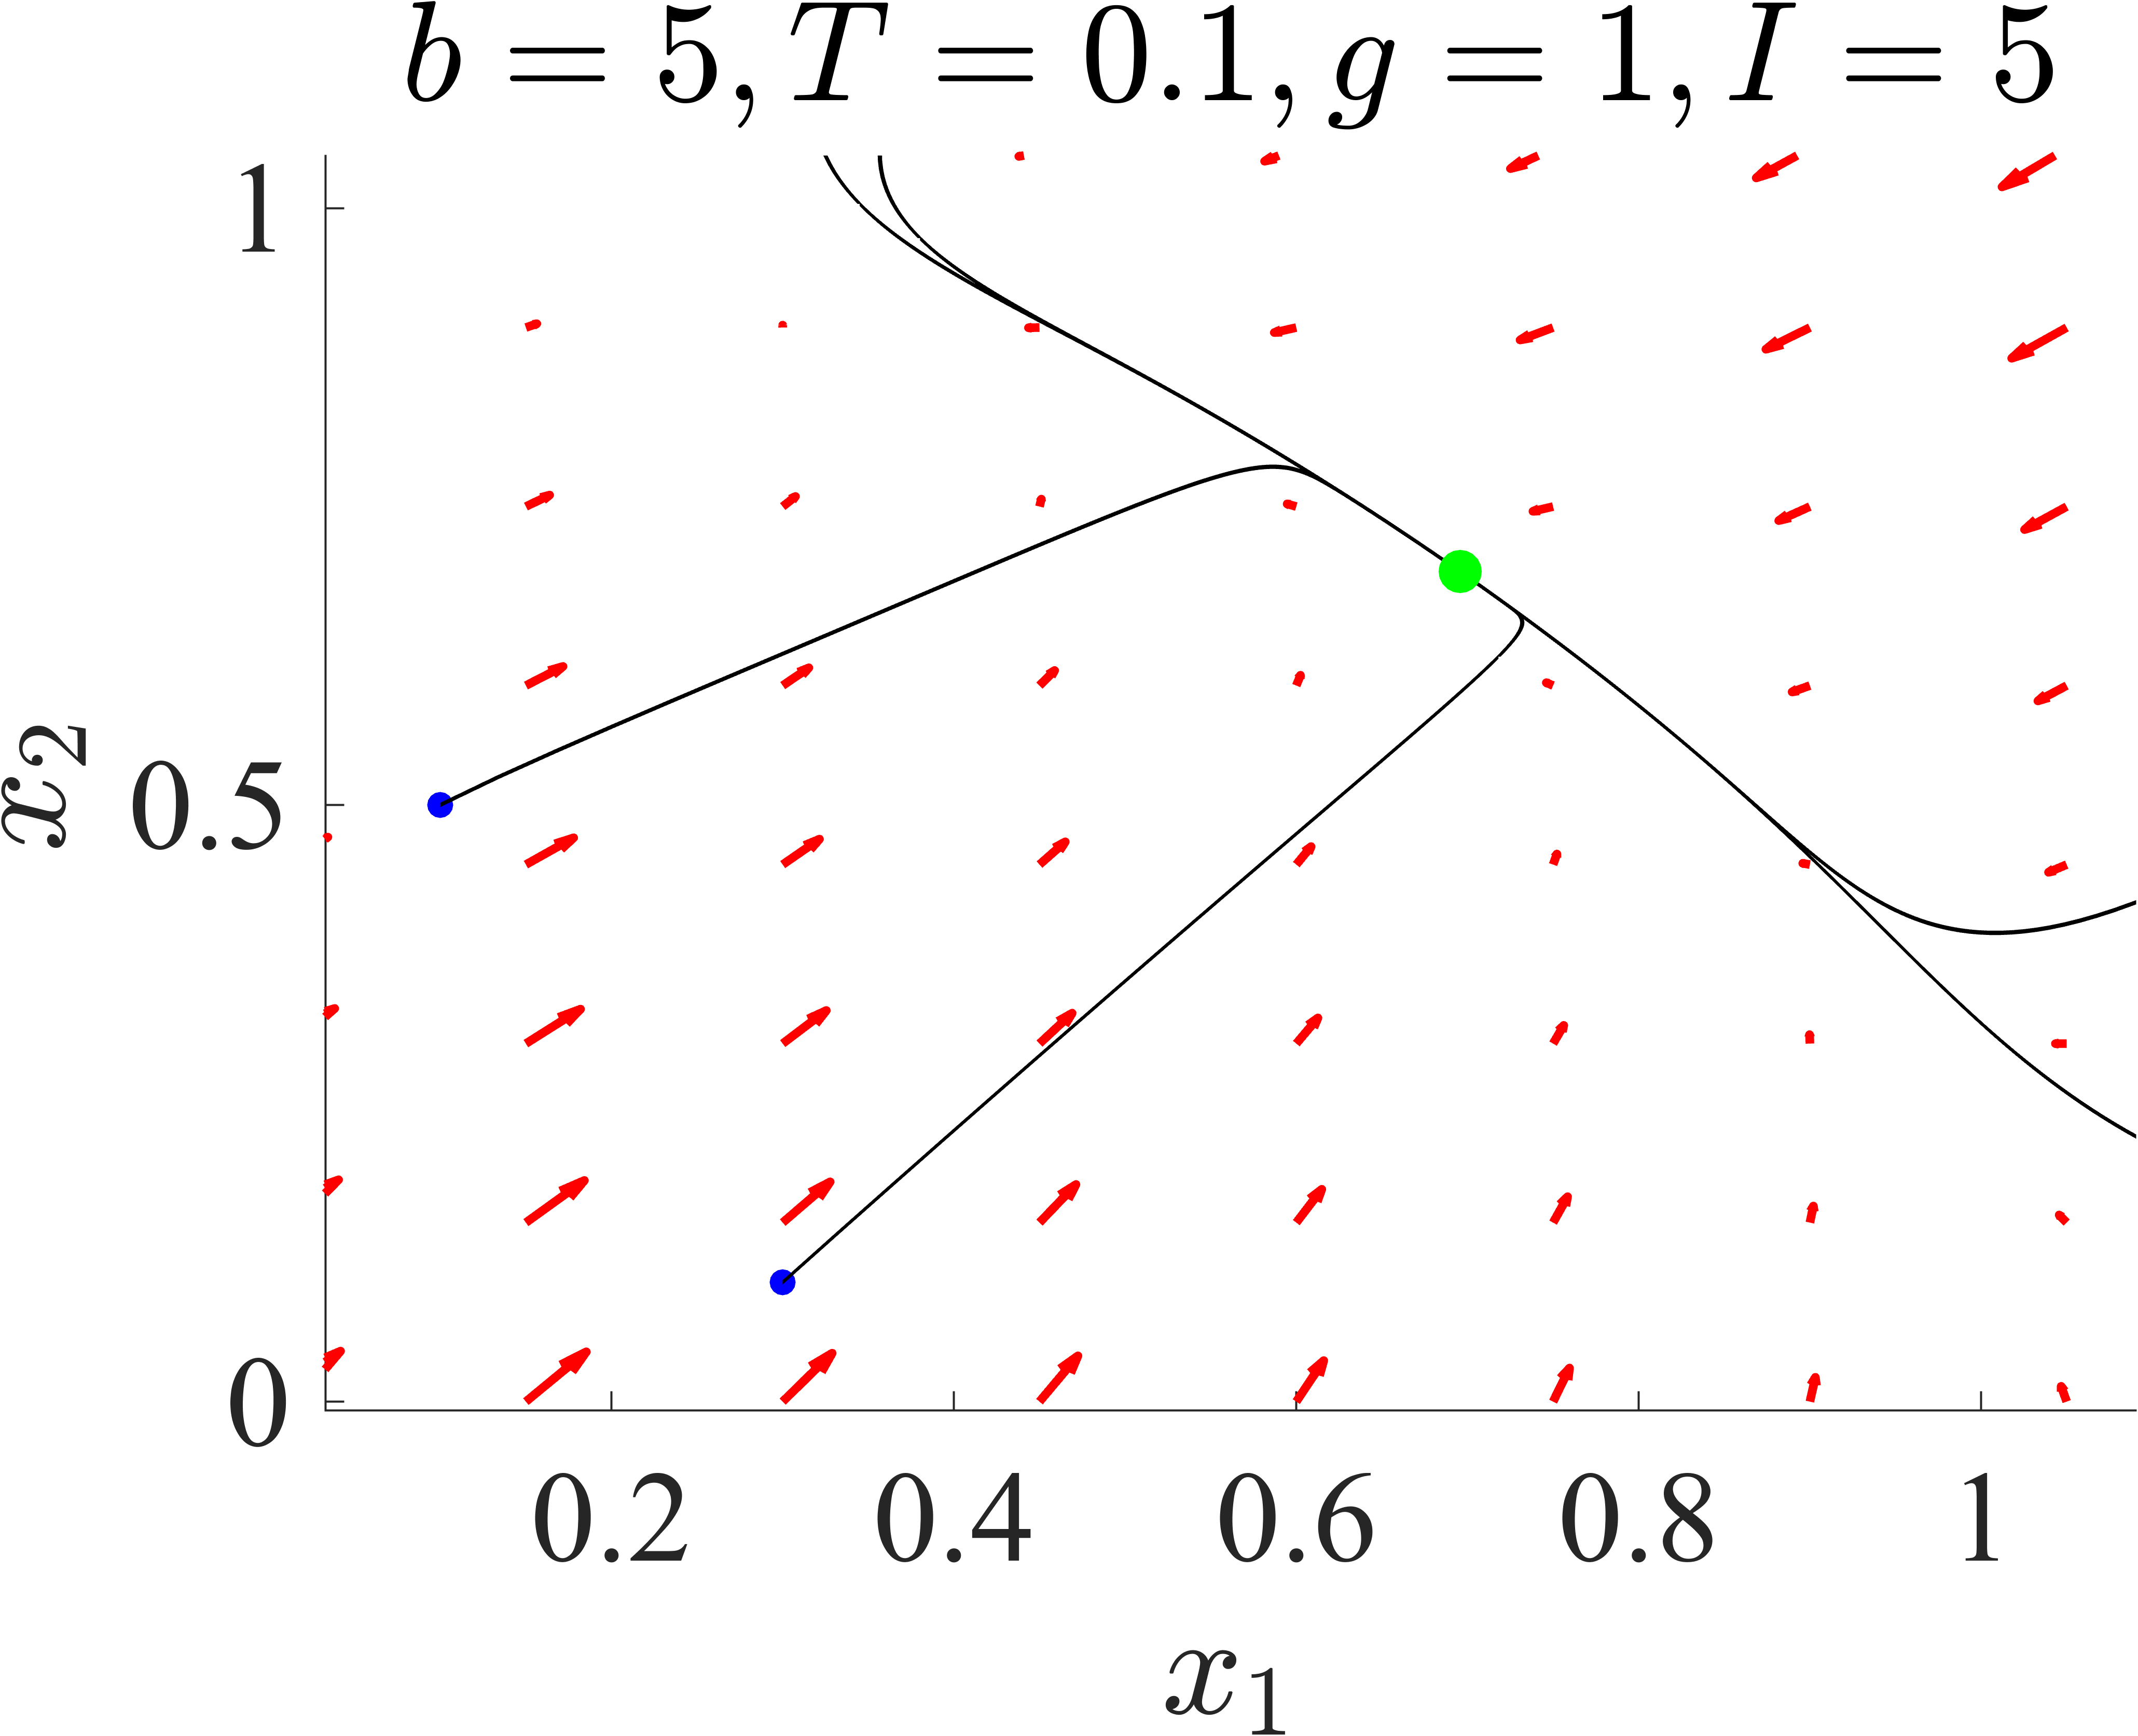
\includegraphics[width=8cm]{xs_HopfNeurons_b_5_T0.1_g1I_5_2.png}
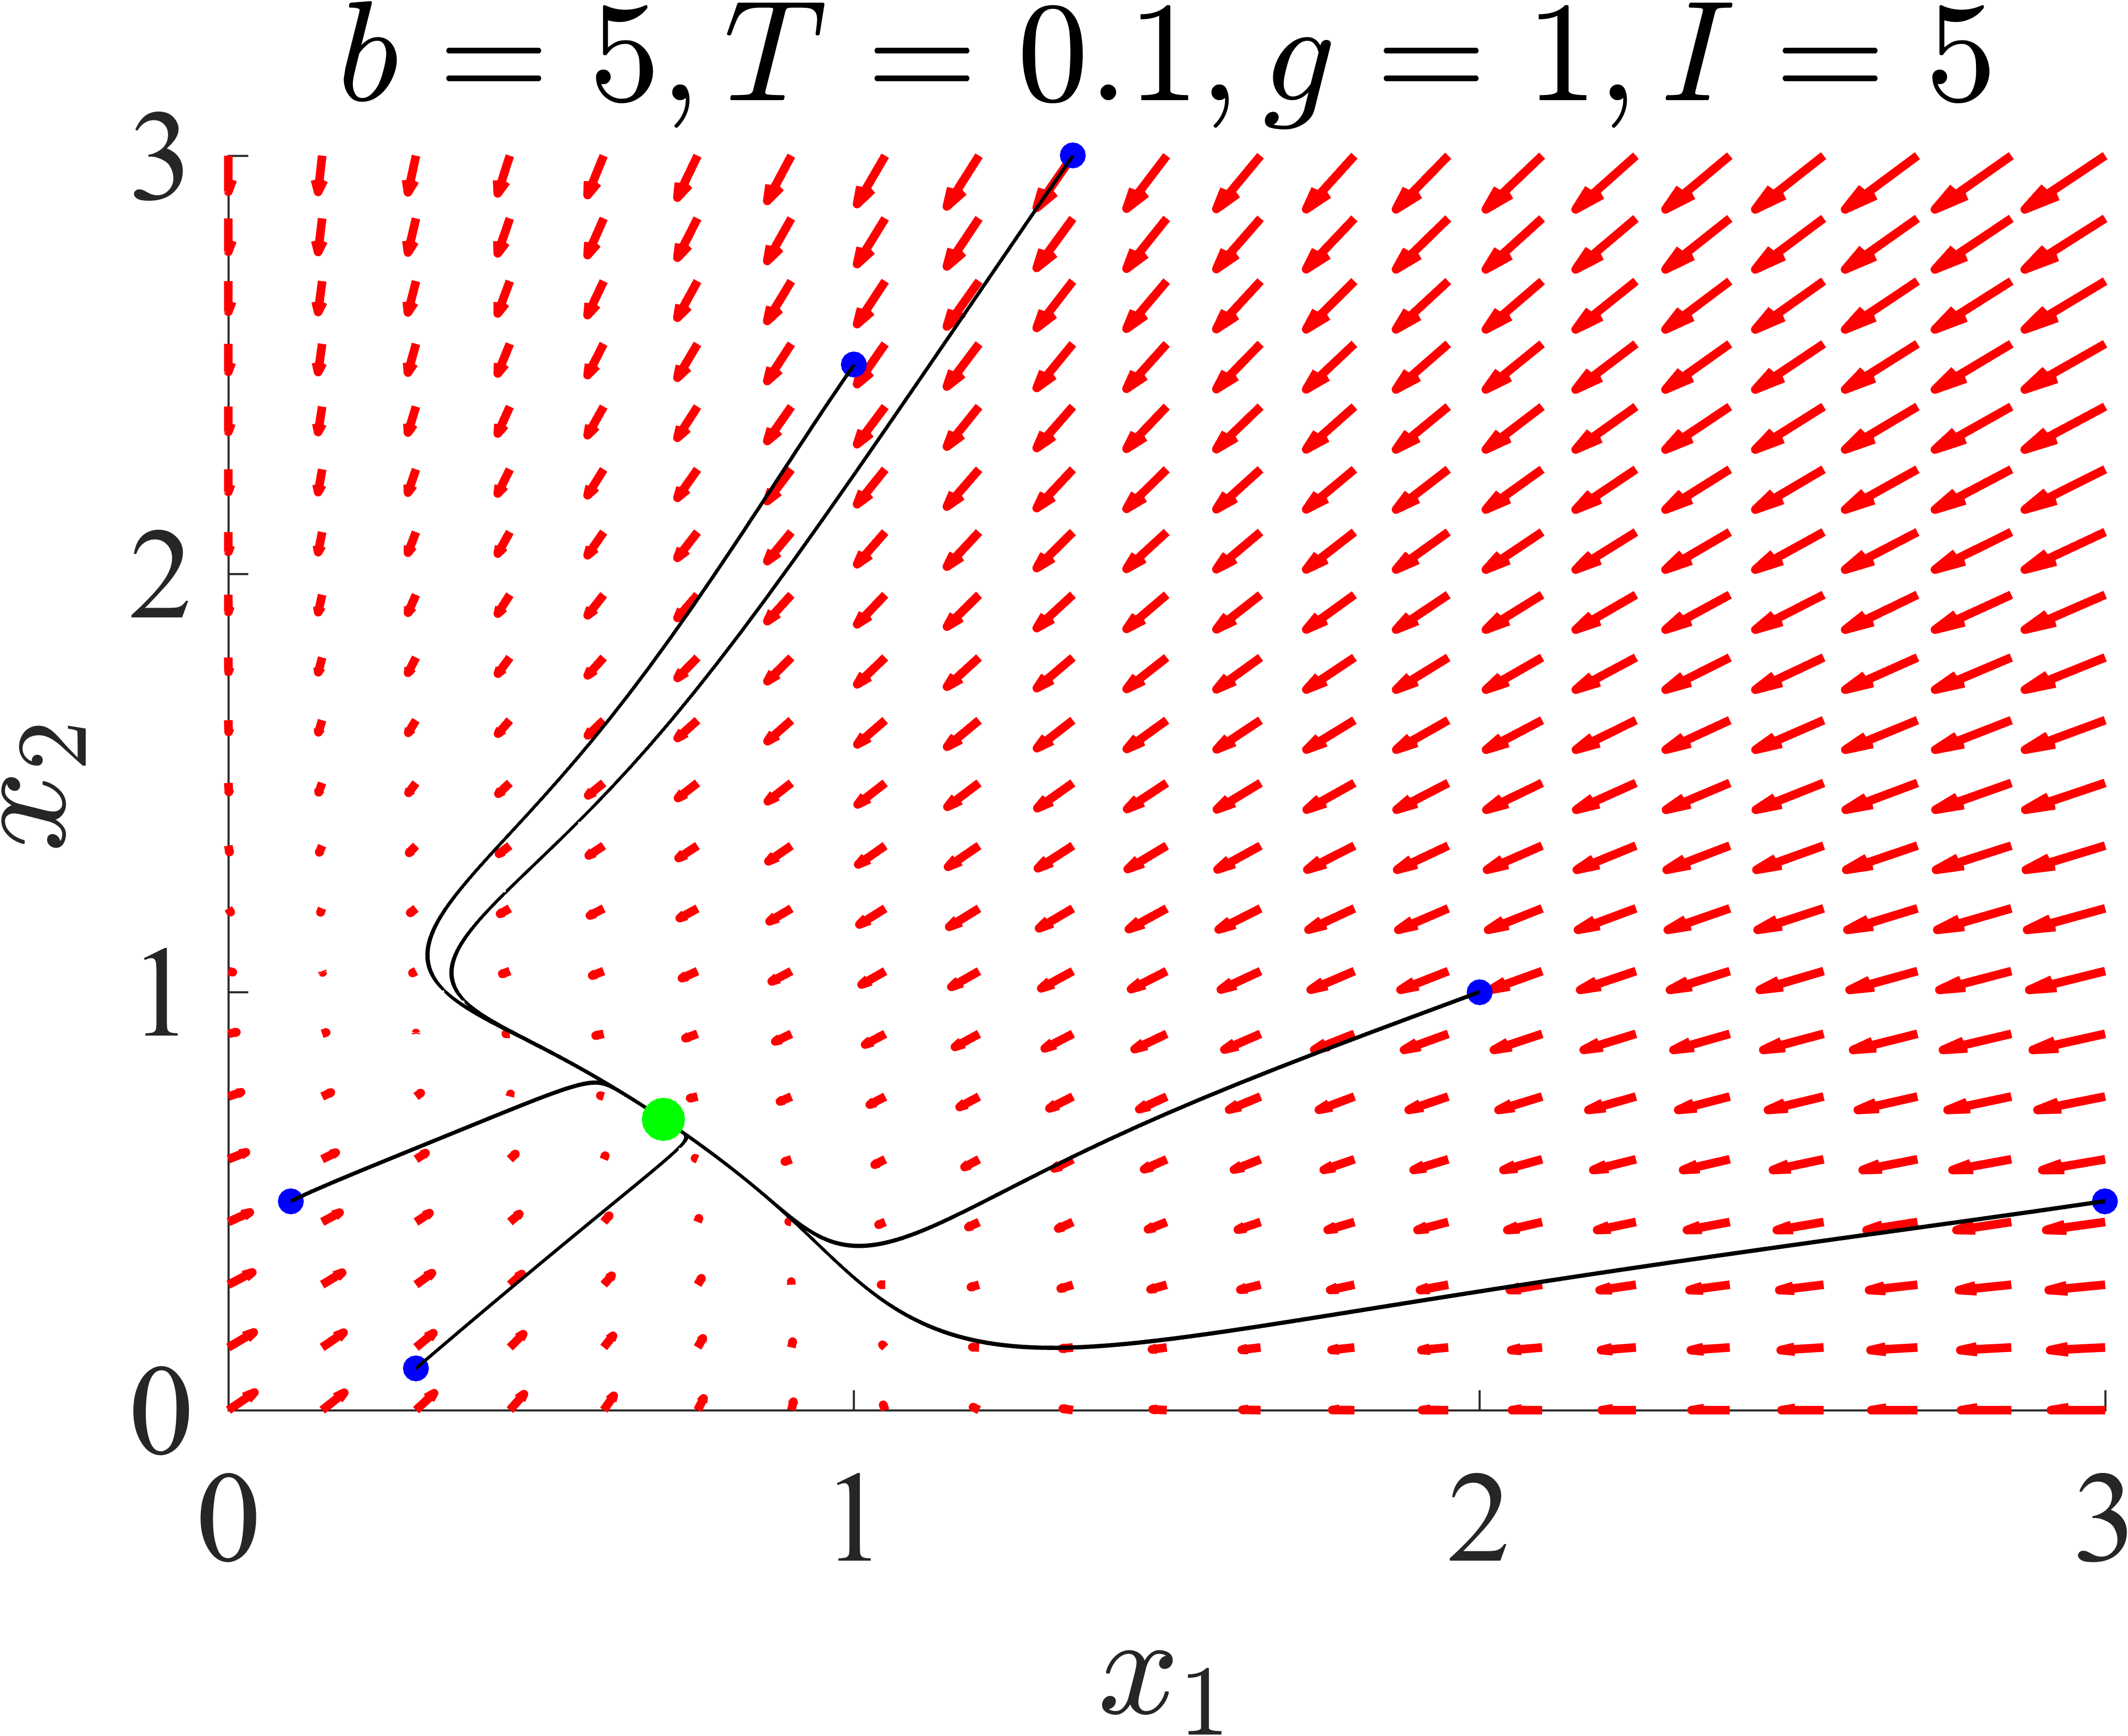
\includegraphics[width=8cm]{xs_HopfNeurons_b_5_T0.1_g1I_5.png}
\caption{Phase Portraits in $x_1$/$x_2$ Plane for Hopf Bifurcation of Binocular Rivalry}
\end{figure}
We predicted that changing the value of $T$, which is the time scale of the adaptations in the $y$-variables building up, will change the sign of the trace of $A-B$ and thus result in a Hopf bifurcation. We see in the figures below that when I set $T = 100$, I seem to have a stable limit cycle around the fixed point (due to the oscillatory pattern) in which we have multiple trajectories spiraling around in that region. Note that the trajectories seem to be on top of each other because we are plotting the projection of the system onto the $x_1/x_2$ plane. We can confirm this by looking at the dynamics in the $y$ variables, as in the next figure (same exact simulation, just plotting dynamics in the other two variables). Here, we see that when $T$ is large, we have lots of oscillations around the same region, indicating the stable limit cycle. When $T$ is small, the trajectories seem to spiral at first but then approach a stable fixed point. We also know that this Hopf bifurcation is supercritical because we transition from a stable spiral (at small $T$) to a stable limit cycle (at large $T$).
\begin{figure}[h]
\centering
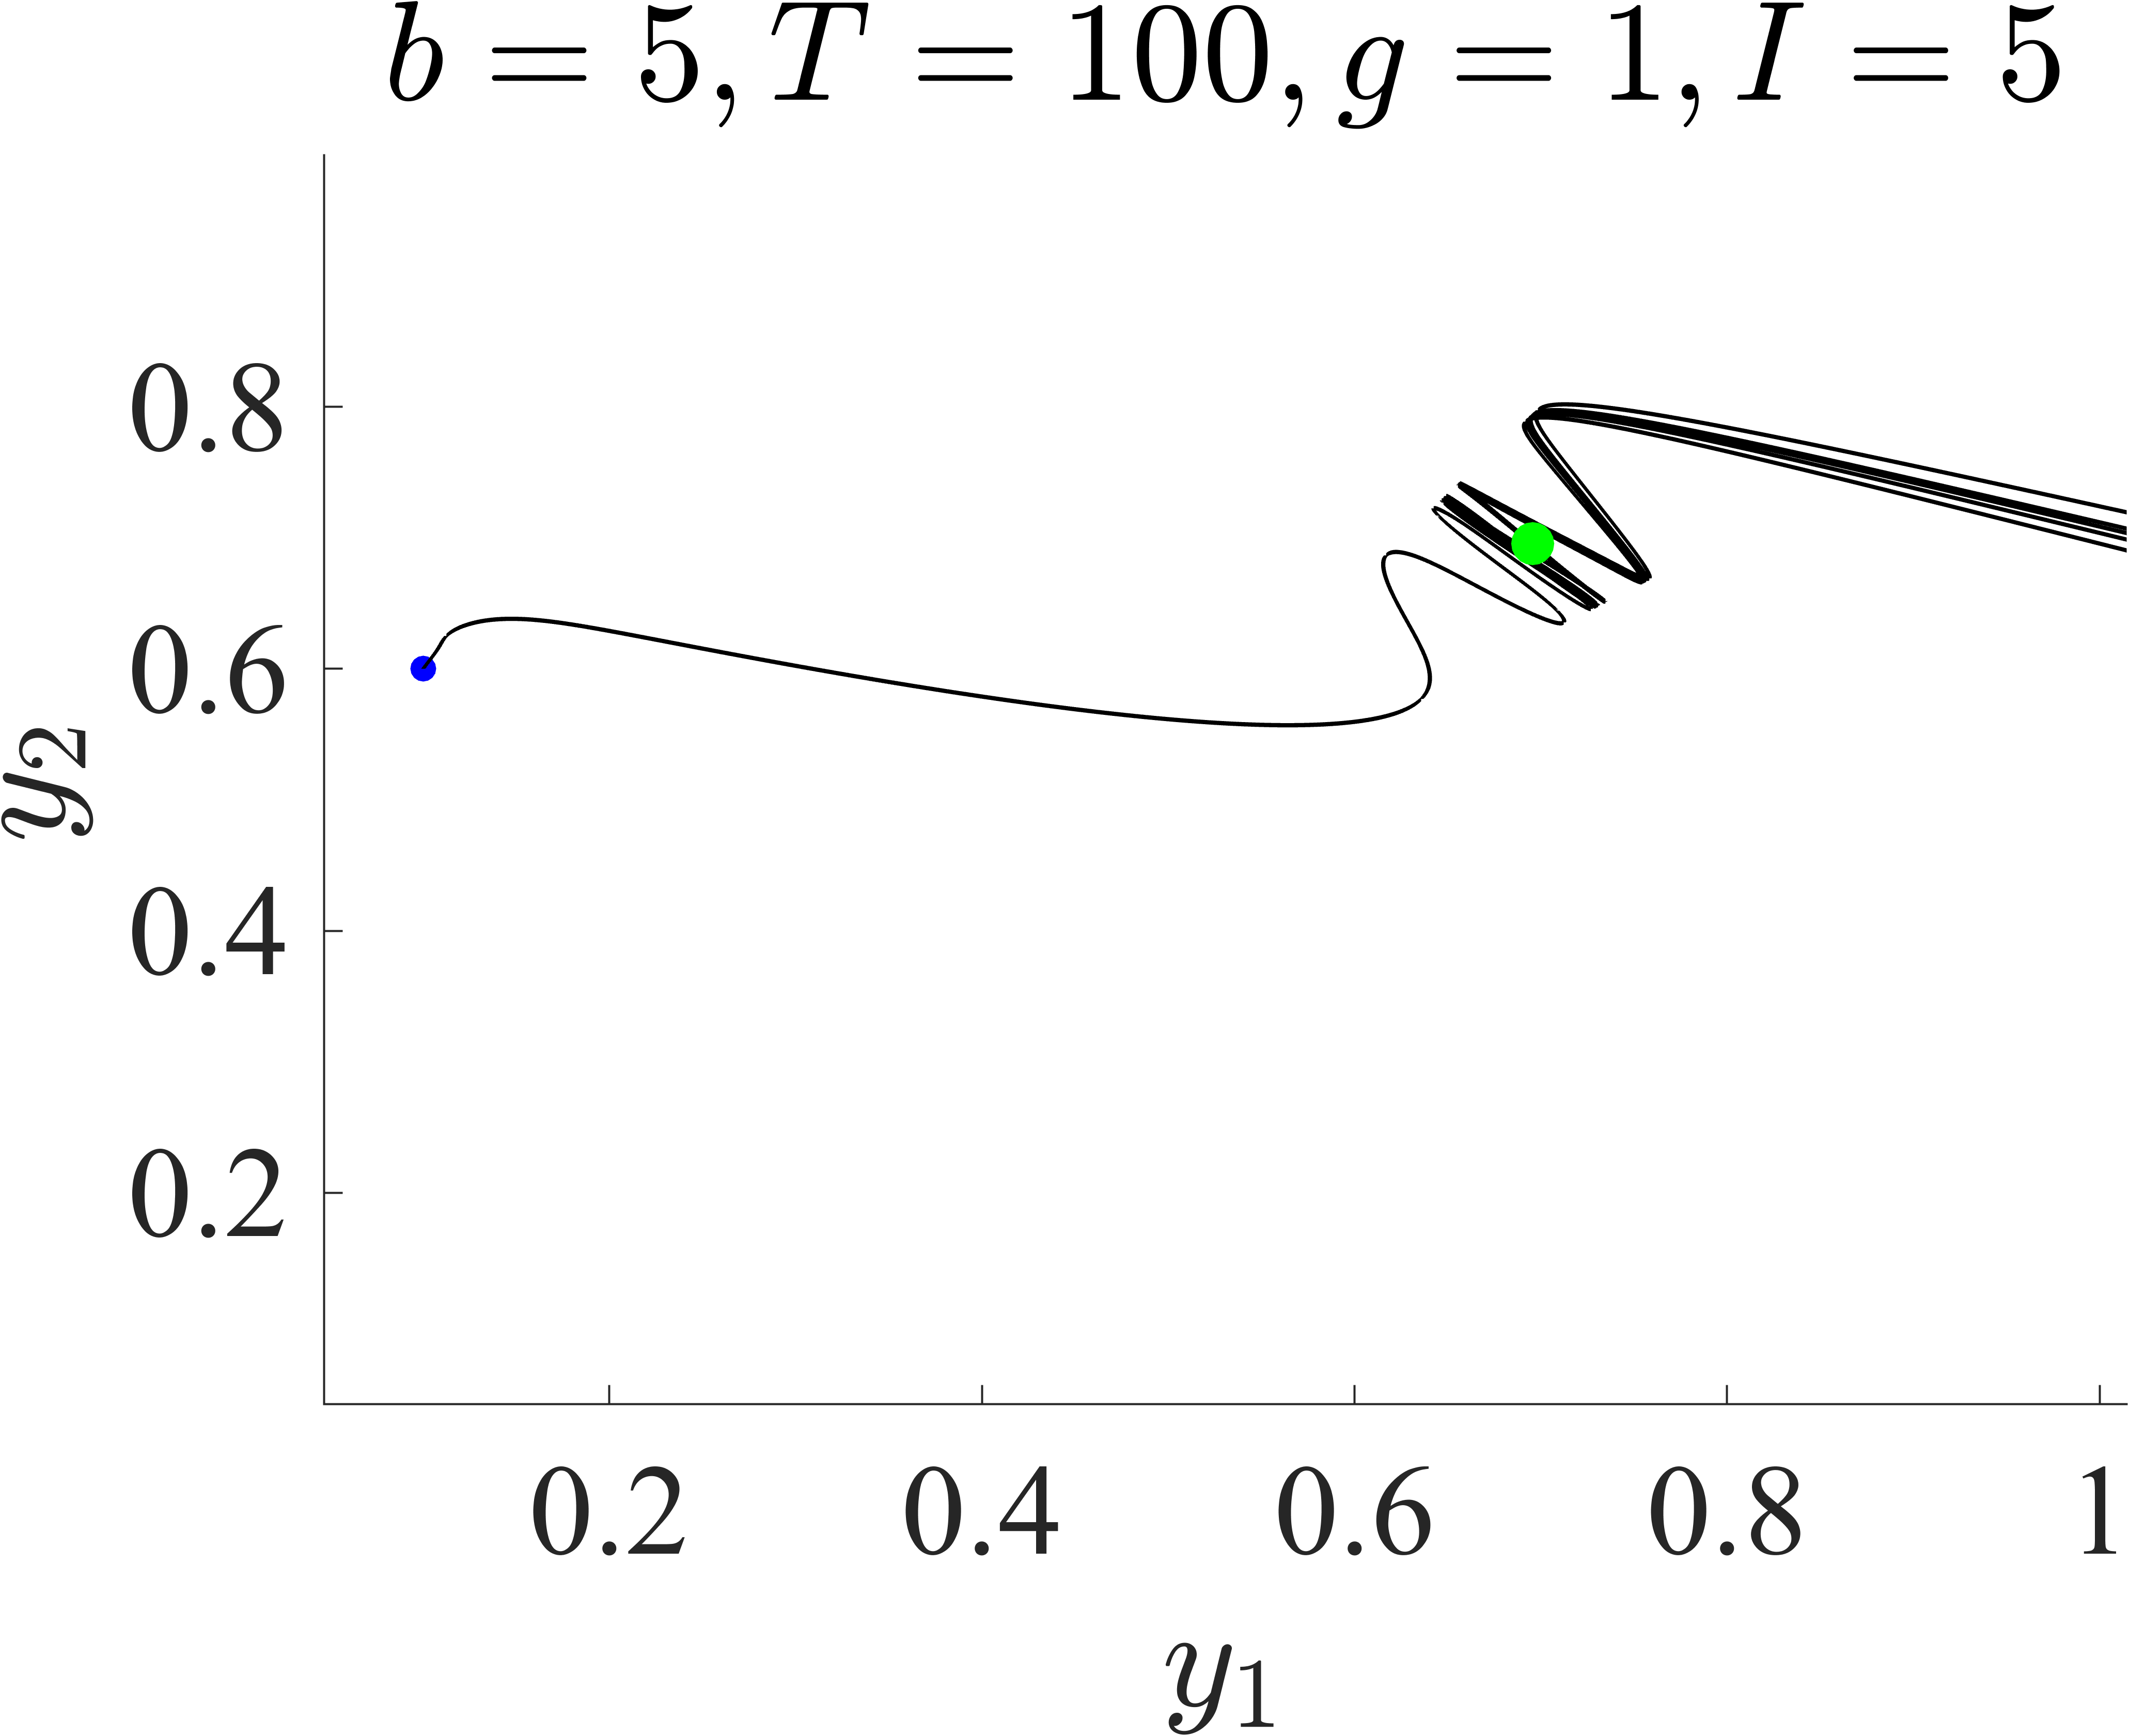
\includegraphics[width=8cm]{ys_HopfNeurons_b_5_T100_g1I_5_2.png}
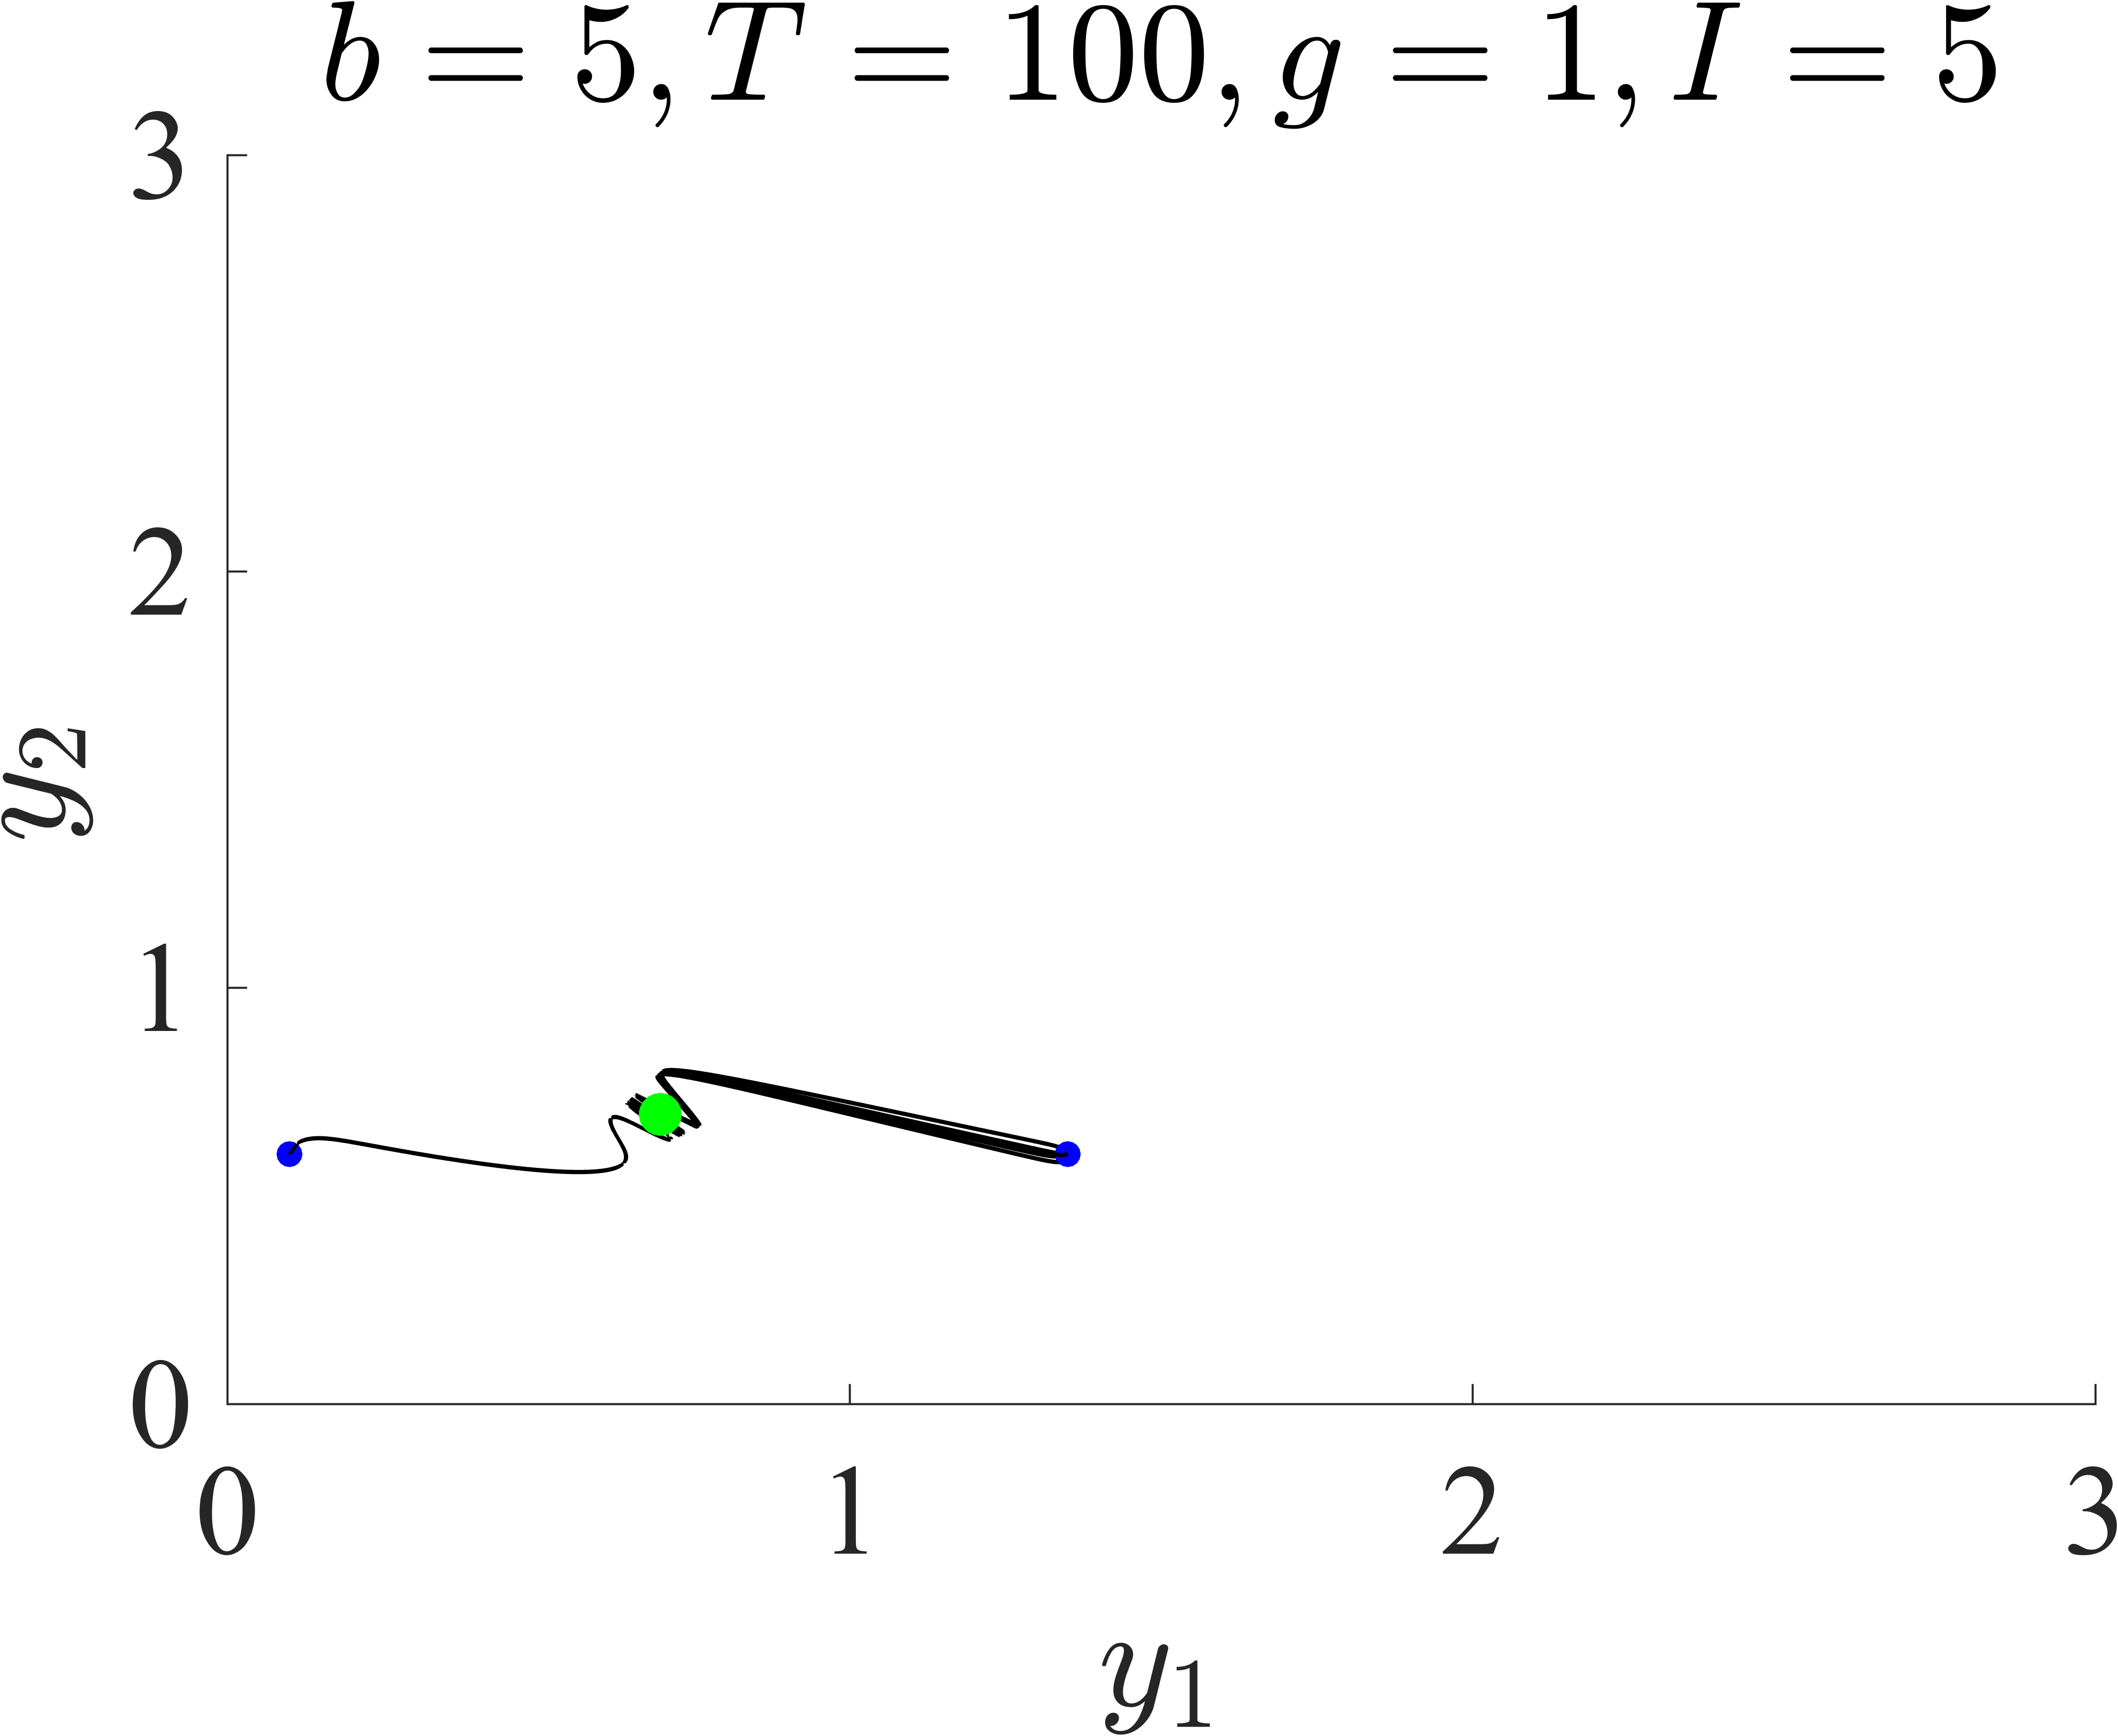
\includegraphics[width=8cm]{ys_HopfNeurons_b_5_T100_g1I_5.png}
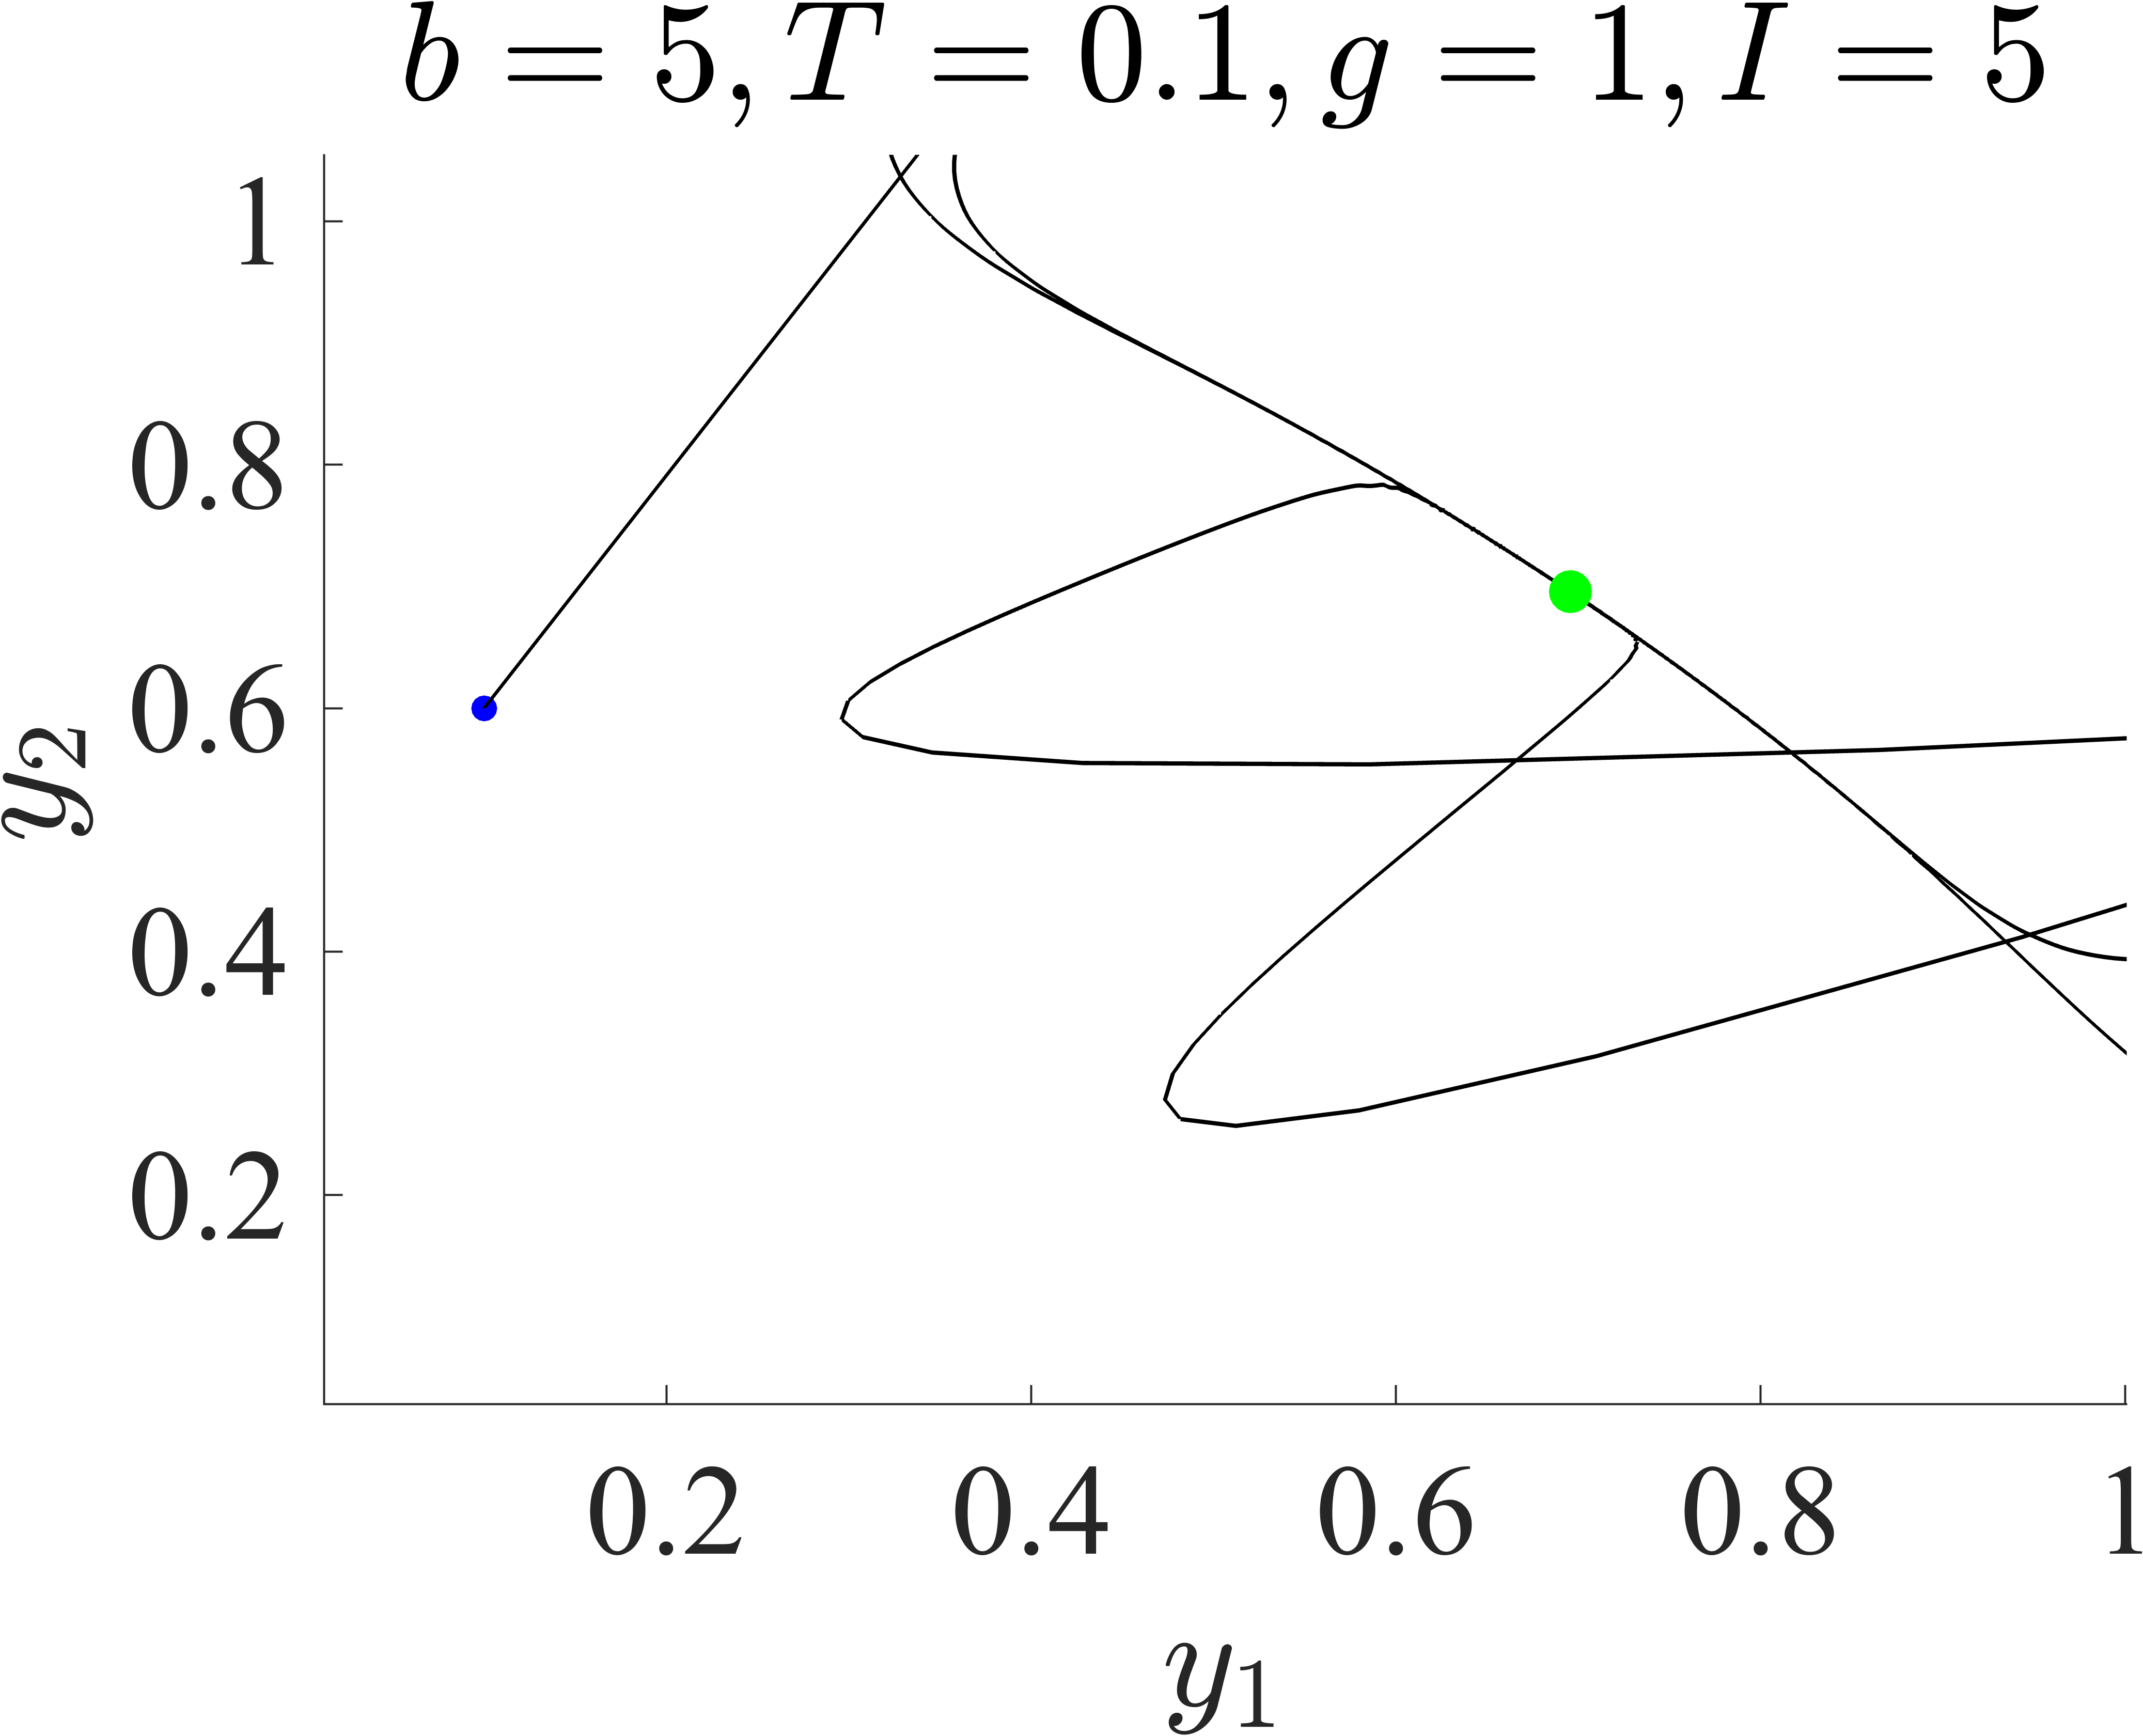
\includegraphics[width=8cm]{ys_HopfNeurons_b_5_T0.1_g1I_5_2.png}
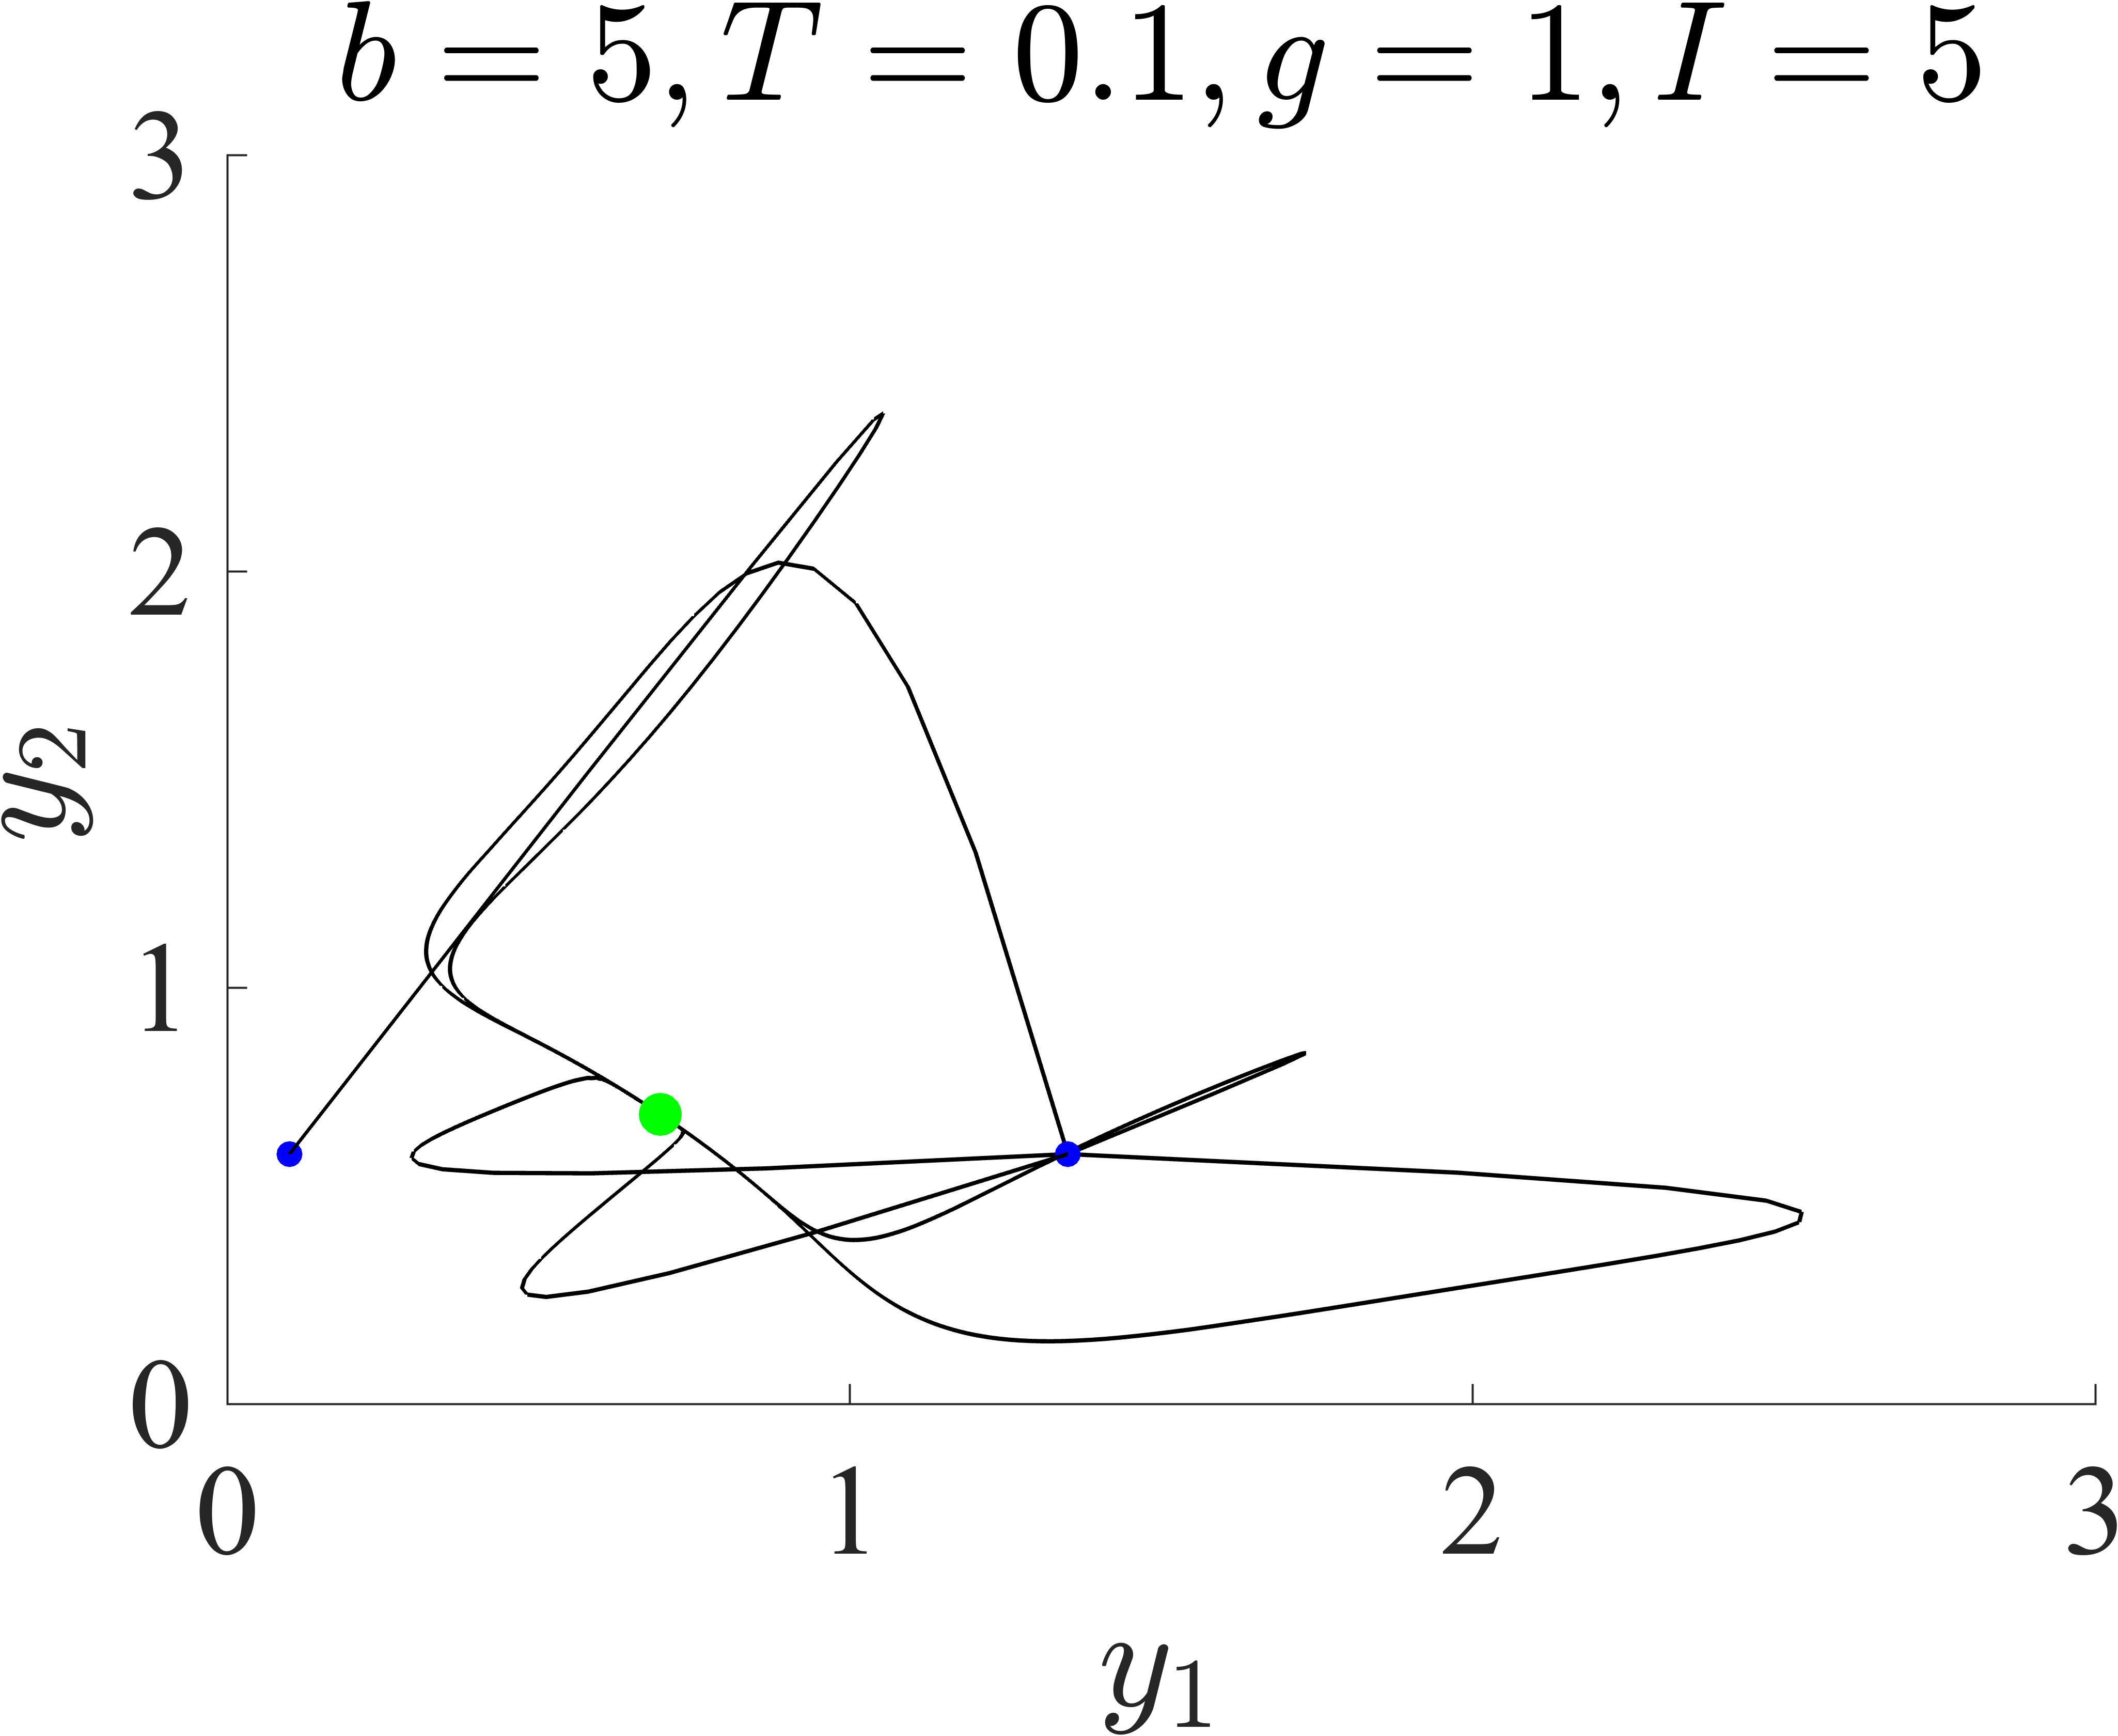
\includegraphics[width=8cm]{ys_HopfNeurons_b_5_T0.1_g1I_5.png}
\caption{Phase Portraits in $y_1$/$y_2$ Plane for Hopf Bifurcation of Binocular Rivalry}
\end{figure}

\section*{Code}
My code is shown below.

\begin{lstlisting}{language=MATLAB}
% 7.3.2

[x,y] = meshgrid(-1.25:.1:1.25,-1.25:.1:1.25);
xdot = x - y - x * (x.^2 + 5 * y.^2);
ydot = x + y - y * (x.^2 + y.^2);

figure()
hold on
quiver(x,y,xdot,ydot,'r','LineWidth',2);
f1 = @ode_732;
plot_solve([.1 0],f1)
plot_solve([-.1 0],f1)
plot_solve([0 .1 ],f1)
plot_solve([0 -.1 ],f1)
plot_solve([1.2 0],f1)
plot_solve([1.2 1.2],f1)
plot_solve([1.2 -1.2],f1)
plot_solve([-1.2 -1.2],f1)
plot_solve([-1.2 1.2],f1)
plot_solve([-1.2 0],f1)
plot_solve([0 1.2],f1)
plot_solve([0 -1.2],f1)
set(gca,'FontSize',30,'FontName','times')
xlabel("$x$",'Interpreter','latex')
ylabel("$y$",'Interpreter','latex')
rectangle('Position',[-1/sqrt(2) -1/sqrt(2) 2.*1/sqrt(2) 2.*1/sqrt(2)],'Curvature',[1 1],'EdgeColor','b','LineWidth',2)
rectangle('Position',[-1 -1 2.*1 2.*1],'Curvature',[1 1],'EdgeColor','b','LineWidth',2)
exportgraphics(gcf,"7.3.2_plot.png","Resolution",600)

%% 8.2.3 
close all
f2 = @ode_823;
mu = 0.01
figure()
hold on
[x,y] = meshgrid(-1:.1:1,-1:.1:1);
xdot = -y + (mu.*x) + (x .* y.^2);
ydot = x + (mu.*y) - (x.^2);
quiver(x,y,xdot,ydot,'r','LineWidth',2);
initial_pos = [.5 .5; .1 0; 0 .1; -.2 0; 0 -.3; 0 0; -.5 -.5; .5 0; 0 .5; .5 .5; -.5 .5; .5 -.5; -.5 0; .95 0; -.8 0; -.6 0];
for i = 1:length(initial_pos)
    scatter(initial_pos(i,1),initial_pos(i,2),'filled','b');
    plot_solve(initial_pos(i,:),f2,mu)
end
xlim([min(x(:)) max(x(:))])
ylim([min(y(:)) max(y(:))])
set(gca,'FontSize',30,'FontName','times')
xlabel("$x$",'Interpreter','latex')
title("$\mu = " + mu + "$",'Interpreter','latex')
ylabel("$y$",'Interpreter','latex')
exportgraphics(gcf,"Hopf_823_phase_mu" + mu + ".png",'Resolution',600)

%% 8.2.4
close all
figure()
hold on
mu = -.01;
rlimcycle = sqrt(-8 * mu);
rs = linspace(0,1.5*rlimcycle,20);
thetas = linspace(0,2*pi,20);
[r, theta] = meshgrid(rs,thetas);
rdot = mu .* r + (1/8) .* r.^3;
thetadot = ones(size(theta));
x = r.* cos(theta);
y = r.* sin(theta);
xdot = rdot .* cos(thetadot) - r .* thetadot .* sin(theta);
ydot = rdot .* sin(thetadot) + r .* thetadot .* cos(theta);
quiver(x,y,xdot,ydot,'r','LineWidth',2);

% in r and theta
initial_pos = rlimcycle.*[0 0; .1 0; .4 0; .9 0; 1.1 0; 1 0; 1.2 pi; 0.95 -pi; 1.05 3*pi/2];
for i = 1:length(initial_pos)
    [xp,yp] = pol2cart(initial_pos(i,2),initial_pos(i,1));
    scatter(xp,yp,'filled','b');
    plot_solve_polar(initial_pos(i,:),mu)
end
set(gca,'FontSize',30,'FontName','times')
hold on
p = nsidedpoly(1000, 'Center', [0 0], 'Radius', rlimcycle);
plot(p, 'EdgeColor', 'g','LineWidth',2,'FaceAlpha',0)
xlim([min(x(:)) max(x(:))])
ylim([min(y(:)) max(y(:))])
xlabel("$x$",'Interpreter','latex')
title("$\mu = " + mu + "$",'Interpreter','latex')
ylabel("$y$",'Interpreter','latex')
exportgraphics(gcf,"Heuristic_824" + mu + ".png",'Resolution',600)

%% 8.2.11

close all
figure()
hold on
[x,y] = meshgrid(-2:.1:2, -2:.1:2);
mu = 0
xdot = y;
ydot = x.^3 - x - mu .* y;
quiver(x,y,xdot,ydot,'r','LineWidth',2);
f1 = @ode_8211;
quiver(x,y,xdot,ydot,'r','LineWidth',2);
% in r and theta
initial_pos = [1.5 0; -1.5 0; 0 -1.5; 0 1.5; 1.5 -1.5; -1.5 1.5; 0 0; -.1 0; .1 .1; -.5 -.5; .3 .3; .9 .9; -.6 0; .6 0; 1 0; -1 0; 0 1; 0 -1; 0 .8; 0 .6; .7 0; .8 0; .9 0; 1.1 0; 0 -.8; 0 -.9; -.8 0; -.7 0; -.9 0; -1.1 0]
for i = 1:length(initial_pos)
    scatter(initial_pos(i,1),initial_pos(i,2),'filled','b');
    plot_solve(initial_pos(i,:),f1,mu);
end
set(gca,'FontSize',30,'FontName','times')
hold on
xlim([min(x(:)) max(x(:))])
ylim([min(y(:)) max(y(:))])
xlabel("$x$",'Interpreter','latex')
title("$\mu = " + mu + "$",'Interpreter','latex')
ylabel("$\dot x$",'Interpreter','latex')
exportgraphics(gcf,"PhasePlot_8211_" + mu + ".png",'Resolution',600)

%% 8.2.17e 
close all
figure(1)
hold on
figure(2)
hold on
tspan = 0:.05:1000;
T = 100;
b = 5;
g = 1;
I = 5;

[x1, y1, x2, y2] = ndgrid([0:.15:3]); 
F = @(x) 1 ./ (1+exp(-x));
x1dot = -x1 + F(I - b.*x2 - g.*y1);
x2dot = -x2 + F(I-b.*x1-g.*y2);
y1i = 10;
y2i = 5;
figure(1)
quiver(x1(:,y1i,:,y2i),x2(:,y1i,:,y2i),x1dot(:,y1i,:,y2i),x2dot(:,y1i,:,y2i),'r','LineWidth',2);

y1o = y1(y1i,y1i,y1i,y1i)
y2o = y2(y2i,y2i,y2i,y2i);
initial_pos = [1 y1o 2.5 y2o; 2 y1o 1 y2o; y1o .1 3 y2o; 3 y1o .5 y2o; .1 y1o .5 y2o;.3 y1o .1 y2o];
for i = 1:length(initial_pos)
    
    y0 = initial_pos(i,:);
    [~,sol] = ode45(@(t,y) ode_8217(t,y,b,g,T,I),tspan,y0);
    figure(1)
    scatter(y0(1),y0(3),'filled','b');
    plot(sol(:,1), sol(:,3),'k','LineWidth',1);

    figure(2)
    scatter(y0(2),y0(4),'filled','b');
    plot(sol(:,2), sol(:,4),'k','LineWidth',1);
end

% Solve for fixed point
syms u
ustar = solve(F(I - b.*u - g.*u) == u, u);

figure(1)
xlim([min(x1(:)) max(x1(:))])
ylim([min(x2(:)) max(x2(:))])
set(gca,'FontSize',30,'FontName','times')
hold on
xlabel("$x_1$",'Interpreter','latex')
ylabel("$x_2$",'Interpreter','latex')
scatter(ustar,ustar,100,"g",'filled');

figure(2)
xlim([min(y1(:)) max(y1(:))])
ylim([min(y2(:)) max(y2(:))])
set(gca,'FontSize',30,'FontName','times')
hold on
xlabel("$y_1$",'Interpreter','latex')
ylabel("$y_2$",'Interpreter','latex')
scatter(ustar,ustar,100,"g",'filled');

figure(1)
title("$b = " + b + ",T = " + T  + ",g = " + g + ",I = " + I + "$",'Interpreter','latex')
exportgraphics(gcf,"xs_HopfNeurons_b_" + b + "_T" + T + "_g" + g+ "I_" + I + ".png",'Resolution',600)

figure(2)
title("$b = " + b + ",T = " + T  + ",g = " + g + ",I = " + I + "$",'Interpreter','latex')
exportgraphics(gcf,"ys_HopfNeurons_b_" + b + "_T" + T + "_g" + g+ "I_" + I + ".png",'Resolution',600)

function plot_solve(y0, myode,mu)
    tspan = 0:.01:100;
    [~,sol] = ode45(@(t,y) myode(t,y,mu),tspan,y0);
    plot(sol(:,1), sol(:,2),'k','LineWidth',1);
end 
function plot_solve_polar(y0,mu)
    tspan = 0:.1:100;    
    % y vector here has r and theta 
    [~,sol] = ode45(@(t,y) ode_polar_824(t,y,mu),tspan,y0);
    % Convert solution from polar coor to cartesian coor 
    x = sol(:,1).* cos(sol(:,2));
    y = sol(:,1).* sin(sol(:,2));
    plot(x,y,'k','LineWidth',1);
end 
function dydt = ode_polar_824(~,yvec,mu)
    % compute polar derivative
    r = yvec(1);
    theta = yvec(2);
    rdot = mu .* r + (1/8) .* r.^3;
    thetadot = ones(size(theta));
    dydt = [rdot; thetadot];
end
function dydt = ode_732(~,yvec)
    x = yvec(1);
    y = yvec(2);
    dydt = [x - y - x * (x.^2 + 5 * y.^2); x + y - y * (x.^2 + y.^2)];
end
function dydt = ode_823(~,yvec,mu)
    x = yvec(1);
    y = yvec(2);
    dydt = [-y + (mu.*x) + (x .* y.^2); x + (mu.*y) - (x.^2)];
end
function dydt = ode_8211(~,yvec,mu)
    x = yvec(1);
    y = yvec(2);
    dydt = [y; x.^3 - x - mu .* y];
end
function dydt = ode_8217(~,yvec,b,g,T,I)
    x1 = yvec(1);
    y1 = yvec(2);
    x2 = yvec(3);
    y2 = yvec(4);
    F = @(x) 1 ./ (1+exp(-x));
    dydt = [-x1 + F(I - b.*x2 - g.*y1); 
            (x1 - y1) ./ T;
            -x2 + F(I-b.*x1-g.*y2);
            (-y2 + x2) ./ T];
end
\end{lstlisting}
\end{document}